\documentclass{article}

\usepackage{url} % Tidy web links
\usepackage{microtype} % 'Improved' typesetting
\usepackage{parskip} % Adds white space between paragraphs
\usepackage[super]{natbib} % Citations using superscript
\usepackage[a4paper, left=2.5cm, right=2.5cm, top=2.5cm, bottom=2.5cm]{geometry}
\usepackage{longtable,booktabs}  % For tables
\usepackage{caption} % For figure and table captions
\usepackage{graphicx} % Adds more functionality to graphics for inclusion of figures
\usepackage{lineno} % Allows use of \linenumbers to add line numbers 
\usepackage[toc,page]{appendix}
\usepackage[utf8]{inputenc}
\frenchspacing % No double spacing between sentences
\linespread{1.2} % Set linespace
\usepackage{authblk} % For author formatting
\usepackage{lmodern} % A scalable font - avoids erros due to non-sclabale fonts
\usepackage{subcaption} % Allows use of subfigures
\DeclareUnicodeCharacter{2060}{\nolinebreak} % Prevent unicode (U+2060) error on local complile
\usepackage{cclicenses} % For creative commons license
\usepackage{verbatim} % Used for word count

% Have different references in Appendix
\usepackage{multibib}
\newcites{appendix}{References for Appendix}

% Choose your own colour
\usepackage{color}
\newcommand{\rmenote}[2][\textcolor{red}{\dagger}]{\textcolor{red}{$#1$}\marginpar{\color{red}\raggedright\tiny$#1$ #2}}
\newcommand{\rmeFIXME}[1]{\textcolor{red}{[\textbf{FIXME} \textsl{#1}]}}
\newcommand{\alnote}[2][\textcolor{blue}{\dagger}]{\textcolor{blue}{$#1$}\marginpar{\color{blue}\raggedright\tiny$#1$ #2}}
\newcommand{\alFIXME}[1]{\textcolor{blue}{[\textbf{FIXME} \textsl{#1}]}}
\newcommand{\kpnote}[2][\textcolor{magenta}{\dagger}]{\textcolor{magenta}{$#1$}\marginpar{\color{magenta}\raggedright\tiny$#1$ #2}}
\newcommand{\kpFIXME}[1]{\textcolor{magenta}{[\textbf{FIXME} \textsl{#1}]}}
\newcommand{\tmnote}[2][\textcolor{green}{\dagger}]{\textcolor{green}{$#1$}\marginpar{\color{green}\raggedright\tiny$#1$ #2}}
\newcommand{\tmFIXME}[1]{\textcolor{green}{[\textbf{FIXME} \textsl{#1}]}}

\hbadness=1000000 % Turn off \hbox badness warnings




\begin{document}

% Info on wordcounts:
% https://www.overleaf.com/learn/how-to/Is_there_a_way_to_run_a_word_count_that_doesn%27t_include_LaTeX_commands%3F

% To include refs in word count:
%TC:incbib

% Ignore title and abstract in word count
%TC:ignore
\title{What would other emergency stroke teams do? Using explainable machine learning to understand variation in thrombolysis practice.}


\renewcommand{\thefootnote}{\fnsymbol{footnote}}
\author[1,2]{Kerry Pearn}
\author[*1,2]{Michael Allen}
\author[1,2]{Anna Laws}
\author[1,2]{Thomas Monks}
\author[4]{Richard Everson}
\author[2,3]{Martin James}

% Check affiliations - update RDE Name
\affil[1]{\footnotesize University of Exeter Medical School}
\affil[2]{\footnotesize NIHR South West Peninsula Applied Research Collaboration (ARC).}
\affil[3]{\footnotesize Royal Devon and Exeter NHS Foundation Trust}
\affil[4]{\footnotesize Computer Science, University of Exeter}
\affil[*]{\footnotesize Corresponding author: m.allen@exeter.ac.uk}
\maketitle

\section{Abstract}

\emph{Objectives}: To understand between-hospital variation in thrombolysis use among emergency stroke admissions in England and Wales.

\emph{Design}: Machine learning was applied to the Sentinel Stroke National Audit Programme (SSNAP)  data set, to learn which patients in each hospital would likely receive thrombolysis.

\emph{Setting}: All hospitals (n=132) providing emergency stroke care in England and Wales. 

\emph{Participants}: 88,928 patients who arrived at hospital within 4 hours of stroke onset, from 2016 to 2018.

\emph{Intervention}: XGBoost machine learning models, with a SHAP model for explainability.

\emph{Main Outcome Measures}: Shapley (SHAP) values, providing estimates of how patient features, and hospital identity, influence the odds of receiving thrombolysis.

\emph{Results}: Thrombolysis use in patients arriving within 4 hours of known or estimated stroke onset ranged 7\%-49\% between hospitals. The odds of receiving thrombolysis reduced 9-fold over the first 120 minutes of arrival-to-scan time, varied 30-fold with stroke severity, reduced 3-fold with estimated rather than precise stroke onset time, fell 6-fold with increasing pre-stroke disability, fell 4-fold with onset during sleep, fell 5-fold with use of anticoagulants, fell 2-fold between 80-110 years of age, reduced 3 fold between 120-240 minutes of onset-to-arrival time, and varied 13-fold between hospitals. The majority of between-hospital variance was explained by the hospital, rather than the differences in local patient populations.

\emph{Conclusions}: Using explainable machine learning, we identified that the majority of the between-hospital variation in thrombolysis use in England and Wales may be explained by differences in in-hospital processes and differences in attitudes to judging suitability for thrombolysis.
%TC:endignore

%\tableofcontents
\newpage
\section{Introduction}

% Include
% 1) What is the problem?
% 2) What do we know about low and varying use of thrombolysis
% 3) What do we not know
% 4) How are we addressing what we don't know

% 1) What is the problem?

Stroke remains one of the leading global causes of death and disability \cite{feigin_global_2021}. Despite reductions in age-standardised rates of stroke, ageing populations are driving an increase in the absolute number of strokes \cite{feigin_global_2021}. Across Europe, in 2017, stroke was found to cost healthcare systems \texteuro 27 billion, or 1.7\% of health expenditure \cite{luengo-fernandez_economic_2020}. Thrombolysis with recombinant tissue plasminogen activator can significantly reduce disability after ischaemic stroke, so long as it is given in the first few hours after stroke onset \cite{emberson_effect_2014}. Despite thrombolysis being of proven benefit in ischaemic stroke, use of thrombolysis varies significantly both between and within European countries \cite{aguiar_de_sousa_access_2019}. In England and Wales the national stroke audit reported that in 2021/22 thrombolysis rates for emergency stroke admissions varied from just 1\% to 28\% between hospitals \cite{sentinel_national_stroke_audit_programme_ssnap_2022}, with a median rate of 10.4\%, against a 2019 NHS England long term plan that 20\% of patients of emergency stroke admissions should be receiving thrombolysis \cite{nhs_long_term_plan_2019}.

% 2) What do we know about low and varying use of thrombolysis

Studies have shown that reasons for low and varying thrombolysis rates are multi-factorial. Reasons include late presentation \cite{aguiar_de_sousa_access_2019}, lack of expertise \cite{aguiar_de_sousa_access_2019} or lack of clear protocols or training \cite{carter-jones_stroke_2011}, delayed access to specialists \cite{kamal_delays_2017}, and poor triage by ambulance or emergency department staff \cite{carter-jones_stroke_2011}. For many factors, the establishment of primary stroke centres has been suggested to improve the emergency care of patients with stroke and reduce barriers to thrombolysis \cite{carter-jones_stroke_2011}, with a centralised model of primary stroke centres leading to increased likelihood of thrombolysis \cite{lahr_proportion_2012, morris_impact_2014, hunter_impact_2013}. 

In addition to organisational factors, clinicians can have varying attitudes to which patients are suitable candidates for thrombolysis. In a discrete choice experiment \cite{de_brun_factors_2018}, the authors concluded that there was considerable heterogeneity among respondents in their thrombolysis decision-making. Areas of difference were around whether to give thrombolysis to mild strokes, to older patients beyond 3 hours from stroke onset, and when there was pre-existing disability.

Based on national audit data from three years of emergency stroke admissions, we have previously built models of the emergency stroke pathway \cite{allen_using_2022, allen_use_2022}, including using machine learning to compare thrombolysis decisions between hospitals. Using these models we found that it would be credible to target an increase in average thrombolysis in England and Wales, from 11\% to 18\%, but that each hospital should have its own target, reflecting differences in local populations. We found that the largest increase in thrombolysis use would come from replicating thrombolysis decision-making practice from higher to lower thrombolysing hospitals. 

% 3) What do we not know

In our previous work we established that we could predict the use of thrombolysis in patients arriving within 4 hours of known stroke onset with 84.3\% accuracy \cite{allen_use_2022}. We could then ask the question ``What if this patient attended another hospital - would they likely be given thrombolysis?" As this was a \emph{`black-box'} decision-forest model we could not effectively explain the relationship between patient level data (`features') and their chance of receiving thrombolysis, or identify and explain the features which different hospitals would differ on.

% 4) How are we addressing what we don't know

In this paper, therefore, we seek to use \emph{explainable machine learning} to understand the relationship between patient and hospital features and the use of thrombolysis across England and Wales, and we seek to understand how hospitals differ in their attitudes to use of thrombolysis, and how much difference in use of thrombolysis may be explained by those differences. We use an \emph{eXtreme Gradient Boosting model \cite{chen_xgboost_2016}} (XGBoost) to make predictions and then use an additional \emph{SHapley Additive exPlanations} \cite{lundberg_unified_2017} (SHAP) model to explain the contribution of each feature to the model prediction.  % Use input instead of include to avoid page break at end
\renewcommand{\thefootnote}{\alph{footnote}} % Use letters for footnotes

\section{Methods}

Note: further details of methods may be found in the online appendix. 

%%%%%%%%%%%%%%%%%%%%%%%%%%%%%%%%%%%%%%%%%%%%%%%%%%%%%%%%%%%%%%%%%%%%%%%%

\subsection{Data}

Data were retrieved for 246,676 emergency stroke admissions to acute stroke teams in England and Wales for the years 2016 - 2018, obtained from the Sentinel Stroke National Audit Programme (SSNAP). Data fields were provided for the hyper-acute phase of the stroke pathway, up to and including our target feature: \emph{receive thrombolysis}. Of these patients, 88,928 arrived within 4 hours of known stroke onset, and were used in this modelling study. The data included 132 acute stroke hospitals.

%%%%%%%%%%%%%%%%%%%%%%%%%%%%%%%%%%%%%%%%%%%%%%%%%%%%%%%%%%%%%%%%%%%%%%%%

\subsection{Machine learning models (to predict thrombolysis use)}

We used an \emph{eXtreme Gradient Boosting model \cite{chen_xgboost_2016}} (`XGBoost') to predict the probability of use of thrombolysis for each patient from their other feature values.

%%%%%%%%%%%%%%%%%%%%%%%%%%%%%%%%%%%%%%%%%%%%%%%%%%%%%%%%%%%%%%%%%%%%%%%%

\subsubsection{Feature selection}

In order to simplify the model (for enhanced explainability) we selected those features most predictive of thrombolysis use. Features were selected by forward-feature selection, identifying one feature at a time that led to the greatest improvement in accuracy as measured by Receiver Operating Characteristic (ROC) Area Under Curve (AUC). We repeated this process to identify the top 25 features, and used these results to identify the number of features to include in our machine learning models.

%%%%%%%%%%%%%%%%%%%%%%%%%%%%%%%%%%%%%%%%%%%%%%%%%%%%%%%%%%%%%%%%%%%%%%%%

\subsubsection{Model accuracy}

Model accuracy, ROC AUC, sensitivity and specificity were measured using stratified 5-fold cross validation. Predicted thrombolysis rate was compared with actual thrombolysis use at hospital-level.

%%%%%%%%%%%%%%%%%%%%%%%%%%%%%%%%%%%%%%%%%%%%%%%%%%%%%%%%%%%%%%%%%%%%%%%%

\subsubsection{Machine learning models}

For the different analysis included in this paper, we trained three XGBoost models:
\begin{enumerate}
    \item \emph{K-fold model}: A 5-fold train-test cross validation used to  test the accuracy of the model, and to test reproducibility of SHAP values.
       
    \item \emph{All data model}: A single model trained on all patients, use to investigate the relationship between feature values and predictions.
    
    \item \emph{10k holdout model}: A model trained all data apart from a 10k hold-out set. This model is used to mimic a 10k cohort of patients that attends all hospitals (by changing the hospital encoding) to further investigate variation in thrombolysis decision-making between hospitals.
\end{enumerate}

%%%%%%%%%%%%%%%%%%%%%%%%%%%%%%%%%%%%%%%%%%%%%%%%%%%%%%%%%%%%%%%%%%%%%%%%
\subsection{SHapley Additive exPlanation (SHAP) values}

We sought to make our models explainable using SHAP values (calculated using the SHAP library \cite{lundberg_unified_2017}). SHAP provides a measure of the contribution of each feature value to the final predicted probability of receiving thrombolysis for that individual. The SHAP values for each feature are comprised of the feature’s main effect (the effect of that feature in isolation) and all of the pairwise interaction effects with each of the other features. SHAP values provide the influence of each feature as the change in log-odds of receiving thrombolysis (SHAP values expressed as log-odds are additive).

%%%%%%%%%%%%%%%%%%%%%%%%%%%%%%%%%%%%%%%%%%%%%%%%%%%%%%%%%%%%%%%%%%%%%%%%
\subsection{The relationship between feature values and the odds of receiving thrombolysis}

For each feature, we examined the relationship between feature values and their corresponding SHAP values (we used values from the \emph{all data} model).

%%%%%%%%%%%%%%%%%%%%%%%%%%%%%%%%%%%%%%%%%%%%%%%%%%%%%%%%%%%%%%%%%%%%%%%%
\subsection{Investigating how the identity of a hospital influences thrombolysis rate}

For each hospital we compared the mean SHAP main effect value for the hospital attended (using values from the \emph{all data} model) with the hospitals observed thrombolysis use.

To reveal the variation in thrombolysis rate due to hospital, rather than patient mix, we also compared the mean hospital attended SHAP main effect value for the identical 10k patient cohort attending each hospital, with the hospitals' predicted thrombolysis use for this 10k patient cohort (we used values from the \emph{10k holdout} model).

%%%%%%%%%%%%%%%%%%%%%%%%%%%%%%%%%%%%%%%%%%%%%%%%%%%%%%%%%%%%%%%%%%%%%%%%

\subsection{Investigating how patient populations and hospital identity and processes influences thrombolysis rate}

The 10 features in the model can be classified into two subsets: 1) `patient descriptive features' (features that describe the patients characteristics), and 2) `hospital descriptive features' (features that describe the hospital’s identity or processes). To analyse the influence that each subset of features has on the thromoblysis rate, we calculated the `subset SHAP value' for each feature, which only includes the components of its SHAP value that contain effects from the features in the same subset. This is expressed as the sum of the main effect and the interaction effects with the other features in the same subset. Multiple regression models were then fitted to the mean subset SHAP values.

%%%%%%%%%%%%%%%%%%%%%%%%%%%%%%%%%%%%%%%%%%%%%%%%%%%%%%%%%%%%%%%%%%%%%%%%

\subsection{Variation in hospital thrombolysis use for patient subgroups}

Informed by the SHAP values, we analysed the observed and predicted use of thrombolysis in eleven subgroups of patients: one subgroup for `ideally' thrombolysable patients, nine `sub-optimal' thrombolysable patient subgroups (one subgroup per feature), and one subgroup with two sub-optimal features The eleven patient subgroups were defined as:

\begin{enumerate}
  \item An \emph{`ideally'} thrombolysable patient:
  \begin{itemize}
    \setlength\itemsep{-2mm}
    \item NIHSS in range 10-25
    \item Arrival-to-scan time $<$30 minutes
    \item Stroke caused by infarction
    \item Precise stroke onset time known
    \item No pre-stroke disability (mRS 0)
    \item Not taking atrial fibrillation anticoagulants
    \item Onset-to-arrival time $<$90 minutes
    \item Age $<$80
    \item Onset not during sleep
  \end{itemize}
  \item NIHSS $<$5
  \item Imprecisely onset time
  \item Existing pre-stroke disability (mRS $>$2)
  \item Haemorrhagic stroke
  \item 60-90 minutes arrival-to-scan time
  \item Patients using AF anticoagulants
  \item 150-180 minutes onset-to-arrival time
  \item Onset during sleep
  \item Age 80+
  \item NIHSS $<$ 5 \emph{and} with estimated stroke onset time
\end{enumerate}

The observed thrombolysis use for each subgroup at each hospital was taken from the SSNAP dataset. In order to further reveal the variation in thrombolysis that was due to hospital decision-making we predicted thrombolysis use for the same patient subgroups at each hospital by using the \emph{10k holdout} model.

%%%%%%%%%%%%%%%%%%%%%%%%%%%%%%%%%%%%%%%%%%%%%%%%%%%%%%%%%%%%%%%%%%%%%%%%

\section{Results}

\subsection{Variation in observed hospital thrombolysis use}

Thrombolysis use in the original data varied between hospitals from 1.5\% to 24.3\% of all patients, and 7.3\% to 49.7\% of patients arriving within 4 hours of known (precise or estimated) stroke onset.

%%%%%%%%%%%%%%%%%%%%%%%%%%%%%%%%%%%%%%%%%%%%%%%%%%%%%%%%%%%%%%%%%%%%%%%%

\subsection{Feature selection}

A model using  10 features had an ROC AUC of 0.923, compared to 0.922 for a model using all available features. We selected 10 features for all subsequent work, which were:

\begin{itemize}
    \item \emph{Arrival-to-scan time} (minutes)
    \item \emph{Infarction}: Stroke type (1 = infarction, 0 = haemorrhage)
    \item \emph{Stroke severity} (NIHSS on arrival)
    \item \emph{Precise onset time} (1 = precise, 0 = best estimate)
    \item \emph{Prior disability level} (modified Rankin Scale, mRS, before stroke)
    \item \emph{Stroke team}
    \item \emph{Use of anticoagulants} *Use of prior anticoagulants; 1 = Yes, 0 = No)
    \item \emph{Onset-to-arrival time} (minutes)
    \item \emph{Onset during sleep }(1 = Yes, 0 = No)
    \item \emph{Age}: (as midpoint of 5 year age bands)
\end{itemize}

Correlations between the 10 features were measured. All r-squared were less than 0.05 except a) age and prior disability level (r-squared 0.146), and b) onset during sleep and precise onset time (r-squared 0.078).

%%%%%%%%%%%%%%%%%%%%%%%%%%%%%%%%%%%%%%%%%%%%%%%%%%%%%%%%%%%%%%%%%%%%%%%%

\subsubsection{Model accuracy}

Model accuracy was measured using stratified 5-fold cross validation. Overall accuracy was 85.0\% (83.9\% sensitivity and specificity could be achieved simultaneously). The model predicted hospital thrombolysis use at each hospital with very good accuracy (r-squared = 0.977, with a mean absolute error of 1.1 percentage points). The appendix contains further model accuracy analysis.

%%%%%%%%%%%%%%%%%%%%%%%%%%%%%%%%%%%%%%%%%%%%%%%%%%%%%%%%%%%%%%%%%%%%%%%%
\subsection{Individual patient SHAP values}
SHAP values are calculated as how they affect log odds of receiving thrombolysis, but for individual predictions, probability values are more intuitive. Figure \ref{fig:results_waterfall} shows \emph{waterfall} plots for example patients with low and high probability of receiving thrombolysis. Waterfall plots show the influence of features for an individual prediction (in our case, patient). The SHAP model starts with a base prediction of a 24\% probability of receiving thrombolysis, before feature values are taken into account. For the patient with a low probability of receiving thrombolysis, the two most influential features reducing the probability of thrombolysis were a long arrival-to-scan time (138 minutes) and a low stroke severity (NIHSS=2). For the patient with a high probability of receiving thrombolysis, the two most influential features increasing the probability of thrombolysis were a short arrival-to-scan time (17 minutes) and a moderate stroke severity (NIHSS=14). 

\begin{figure}%[!ht]
    \caption*{\footnotesize{\textsf{Patient with low probability of receiving thrombolysis}}}
    \vspace{-4mm} % reduce space after caption
    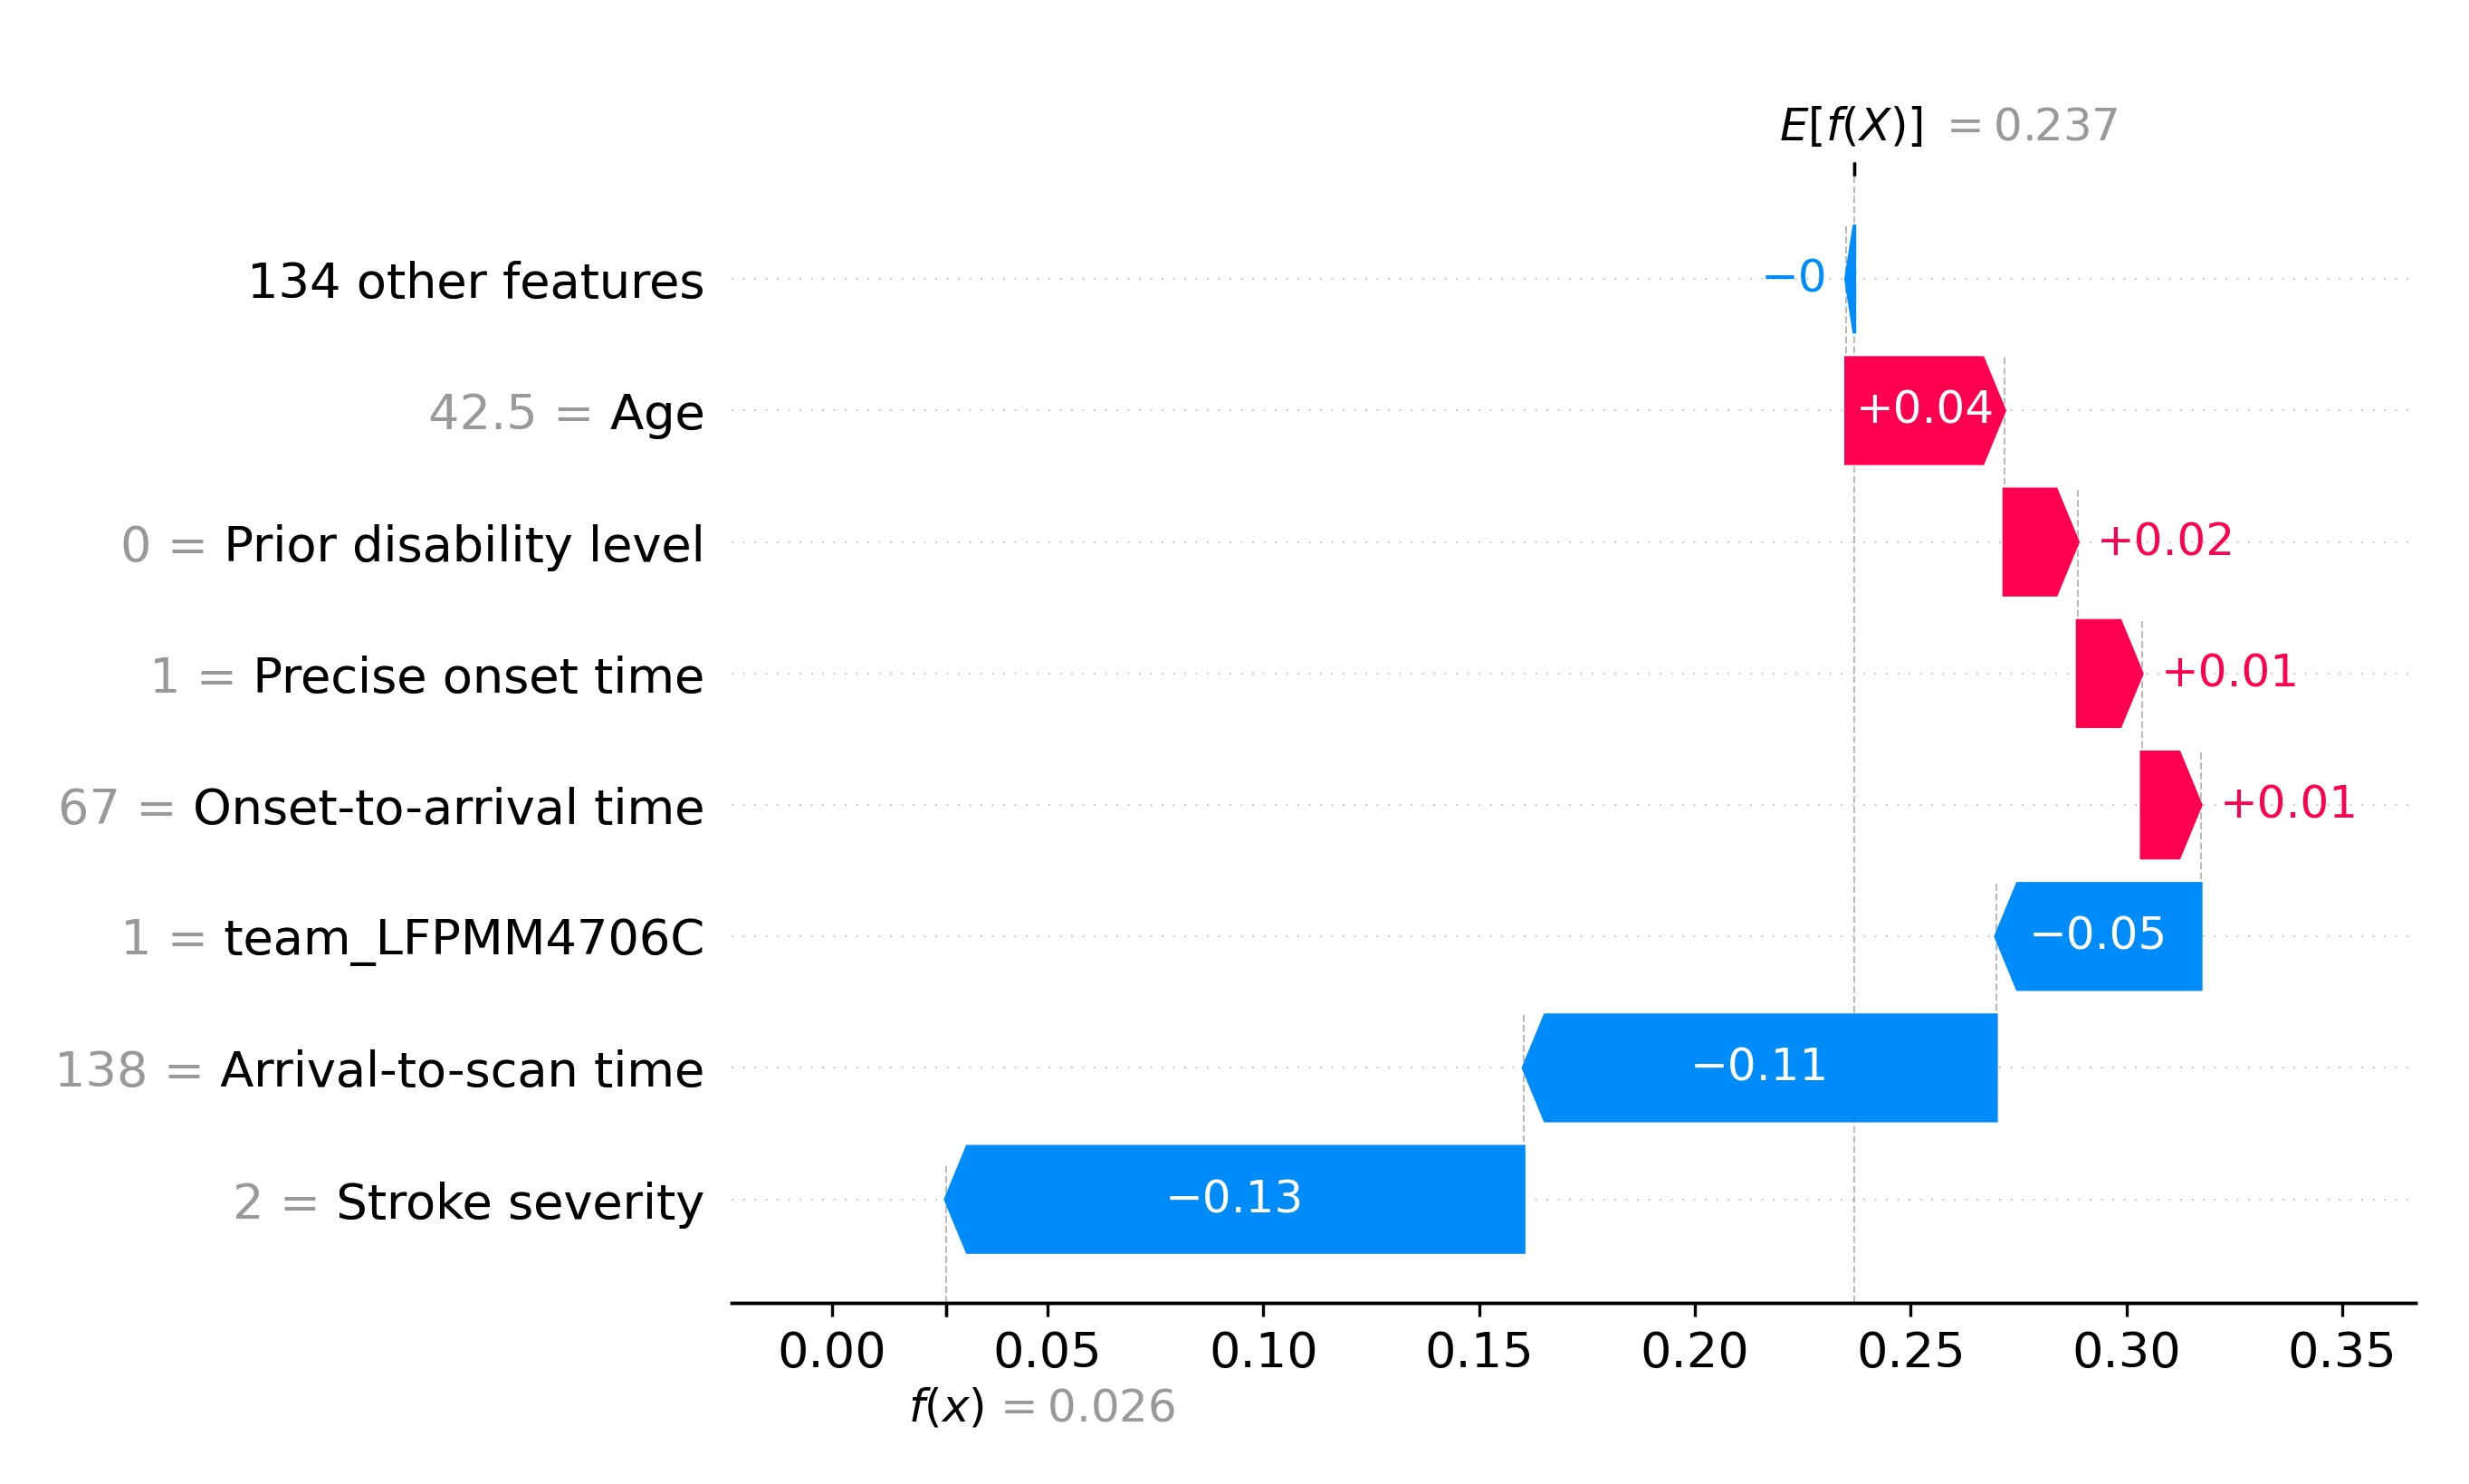
\includegraphics[width=0.75\textwidth]{./images/03_xgb_10_features_waterfall_probability_low}
    \vspace{2mm}
    \caption*{\footnotesize{\textsf{Patient with high probability of receiving thrombolysis}}}
    \vspace{-4mm} % reduce space after caption
    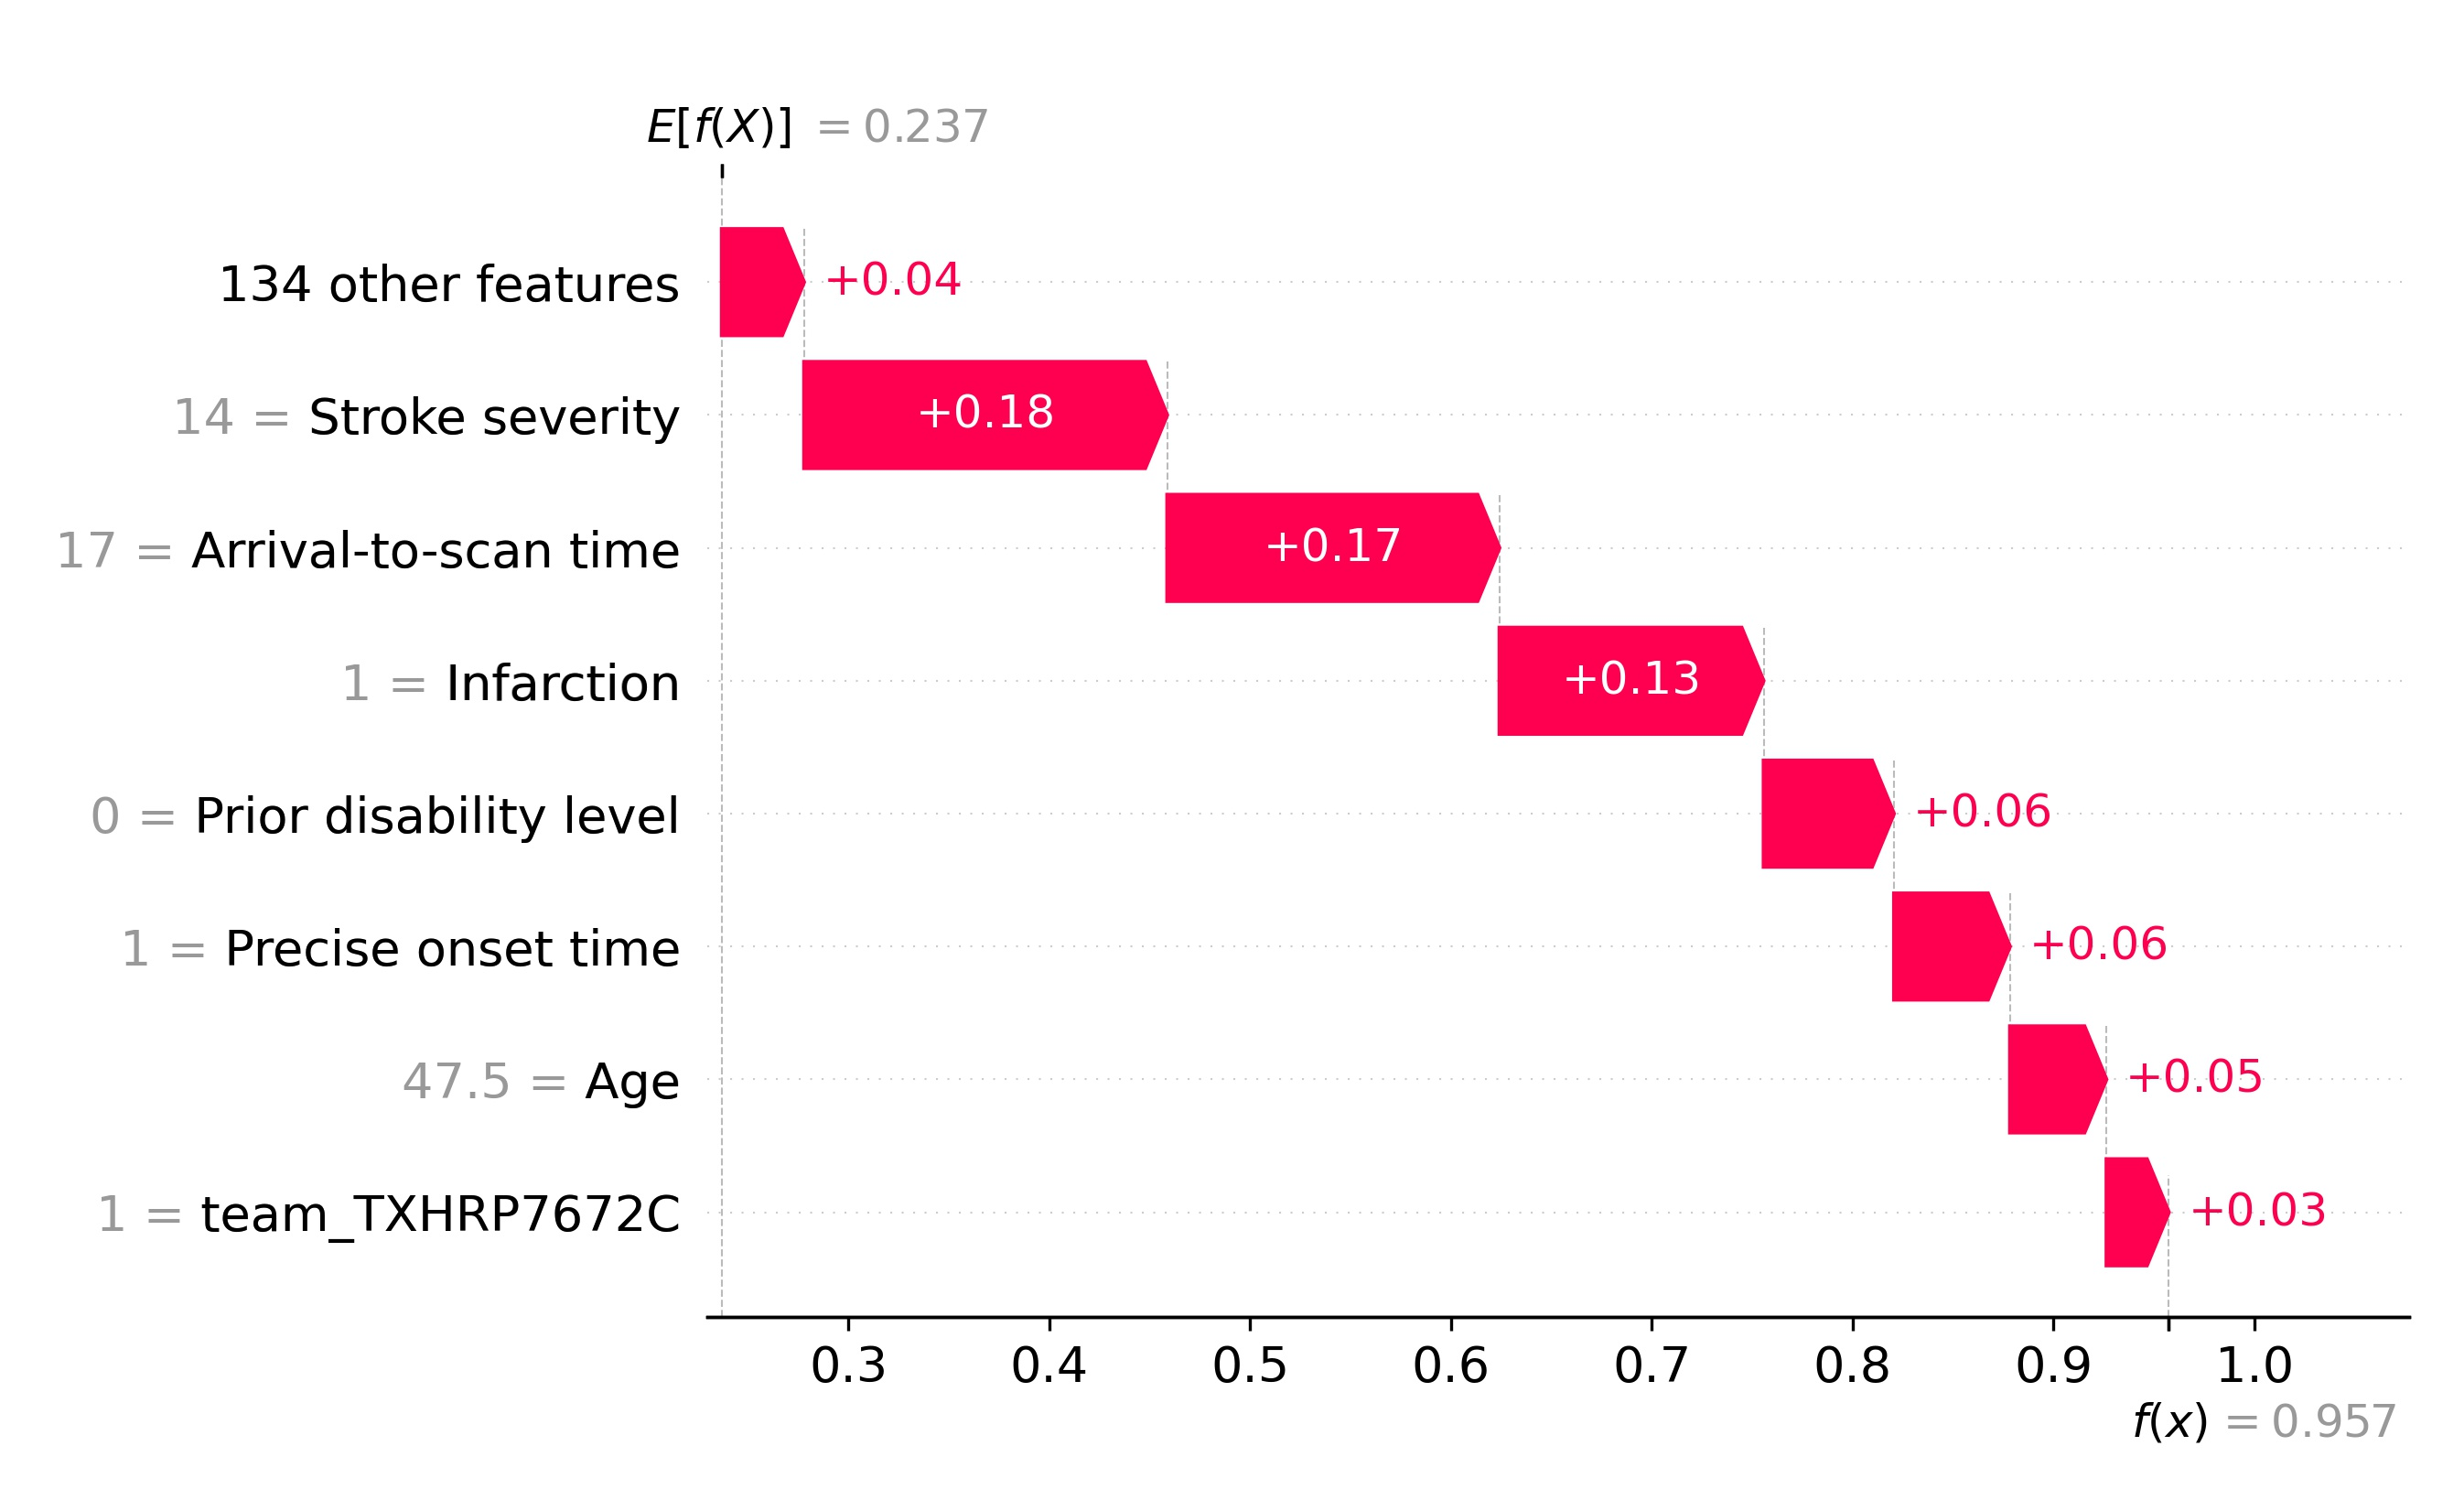
\includegraphics[width=0.75\textwidth]{./images/03_xgb_10_features_waterfall_probability_high}
\caption{Waterfall plots showing the influence of each feature on the predicted probability of a single patient receiving thrombolysis. Top: An example of a patient with a low probability (2.6\%) of receiving thrombolysis. Bottom: An example of a patient with a high probability (95.7\%) of receiving thrombolysis.}
\label{fig:results_waterfall}
\end{figure}

%\newpage
%%%%%%%%%%%%%%%%%%%%%%%%%%%%%%%%%%%%%%%%%%%%%%%%%%%%%%%%%%%%%%%%%%%%%%%%

\subsection{The relationship between feature values and the odds of receiving thrombolysis}

\begin{minipage}{1\textwidth}
Figure \ref{fig:shap_feature_subfigure} shows the relationship between patient level feature values and their SHAP values. Key observations are:

\begin{itemize}
    \item \emph{Stroke type}: The SHAP values for stroke type show that the model effectively eliminated any probability of receiving thrombolysis for haemorrhagic stroke.
    \item \emph{Arrival-to-scan time}: The odds of receiving thrombolysis reduced by 9-fold over the first 120 minutes of arrival-to-scan time.
    \item \emph{Stroke severity (NIHSS)}: The odds of receiving thrombolysis were lowest at NIHSS 0, increased and peaked at NIHSS 15-25, and then fell again with higher stroke severity (NIHSS above 25). The difference between minimum odds and maximum odds of receiving thrombolysis was 30-fold.
    \item \emph{Stroke onset time type}: The odds of receiving thrombolysis were 3-fold greater for precise onset time than estimated onset time.
    \item \emph{Disability level (mRS) before stroke}: The odds of receiving thrombolysis fell 6-fold between mRS 0-5.
    \item \emph{Use of AF anticoagulants}: The odds of receiving thrombolysis were reduced 5-fold with anticoagulant use.
    \item \emph{Onset-to-arrival time}: The odds of receiving thrombolysis were similar below 120 minutes, then fell 3-fold between 120-240 minutes.
    \item \emph{Age}: The odds of receiving thrombolysis were similar below 80 years old, then fell 2-fold between 80-110 years old.    
    \item \emph{Onset during sleep}: The odds of receiving thrombolysis were 4-fold lower for onset during sleep.
    \item \emph{Hospital attended}: There was a 13-fold difference in odds of receiving thrombolysis between hospitals.
\end{itemize}
\end{minipage}

% SHAP violon plots

\begin{figure}%[!h]
\centering
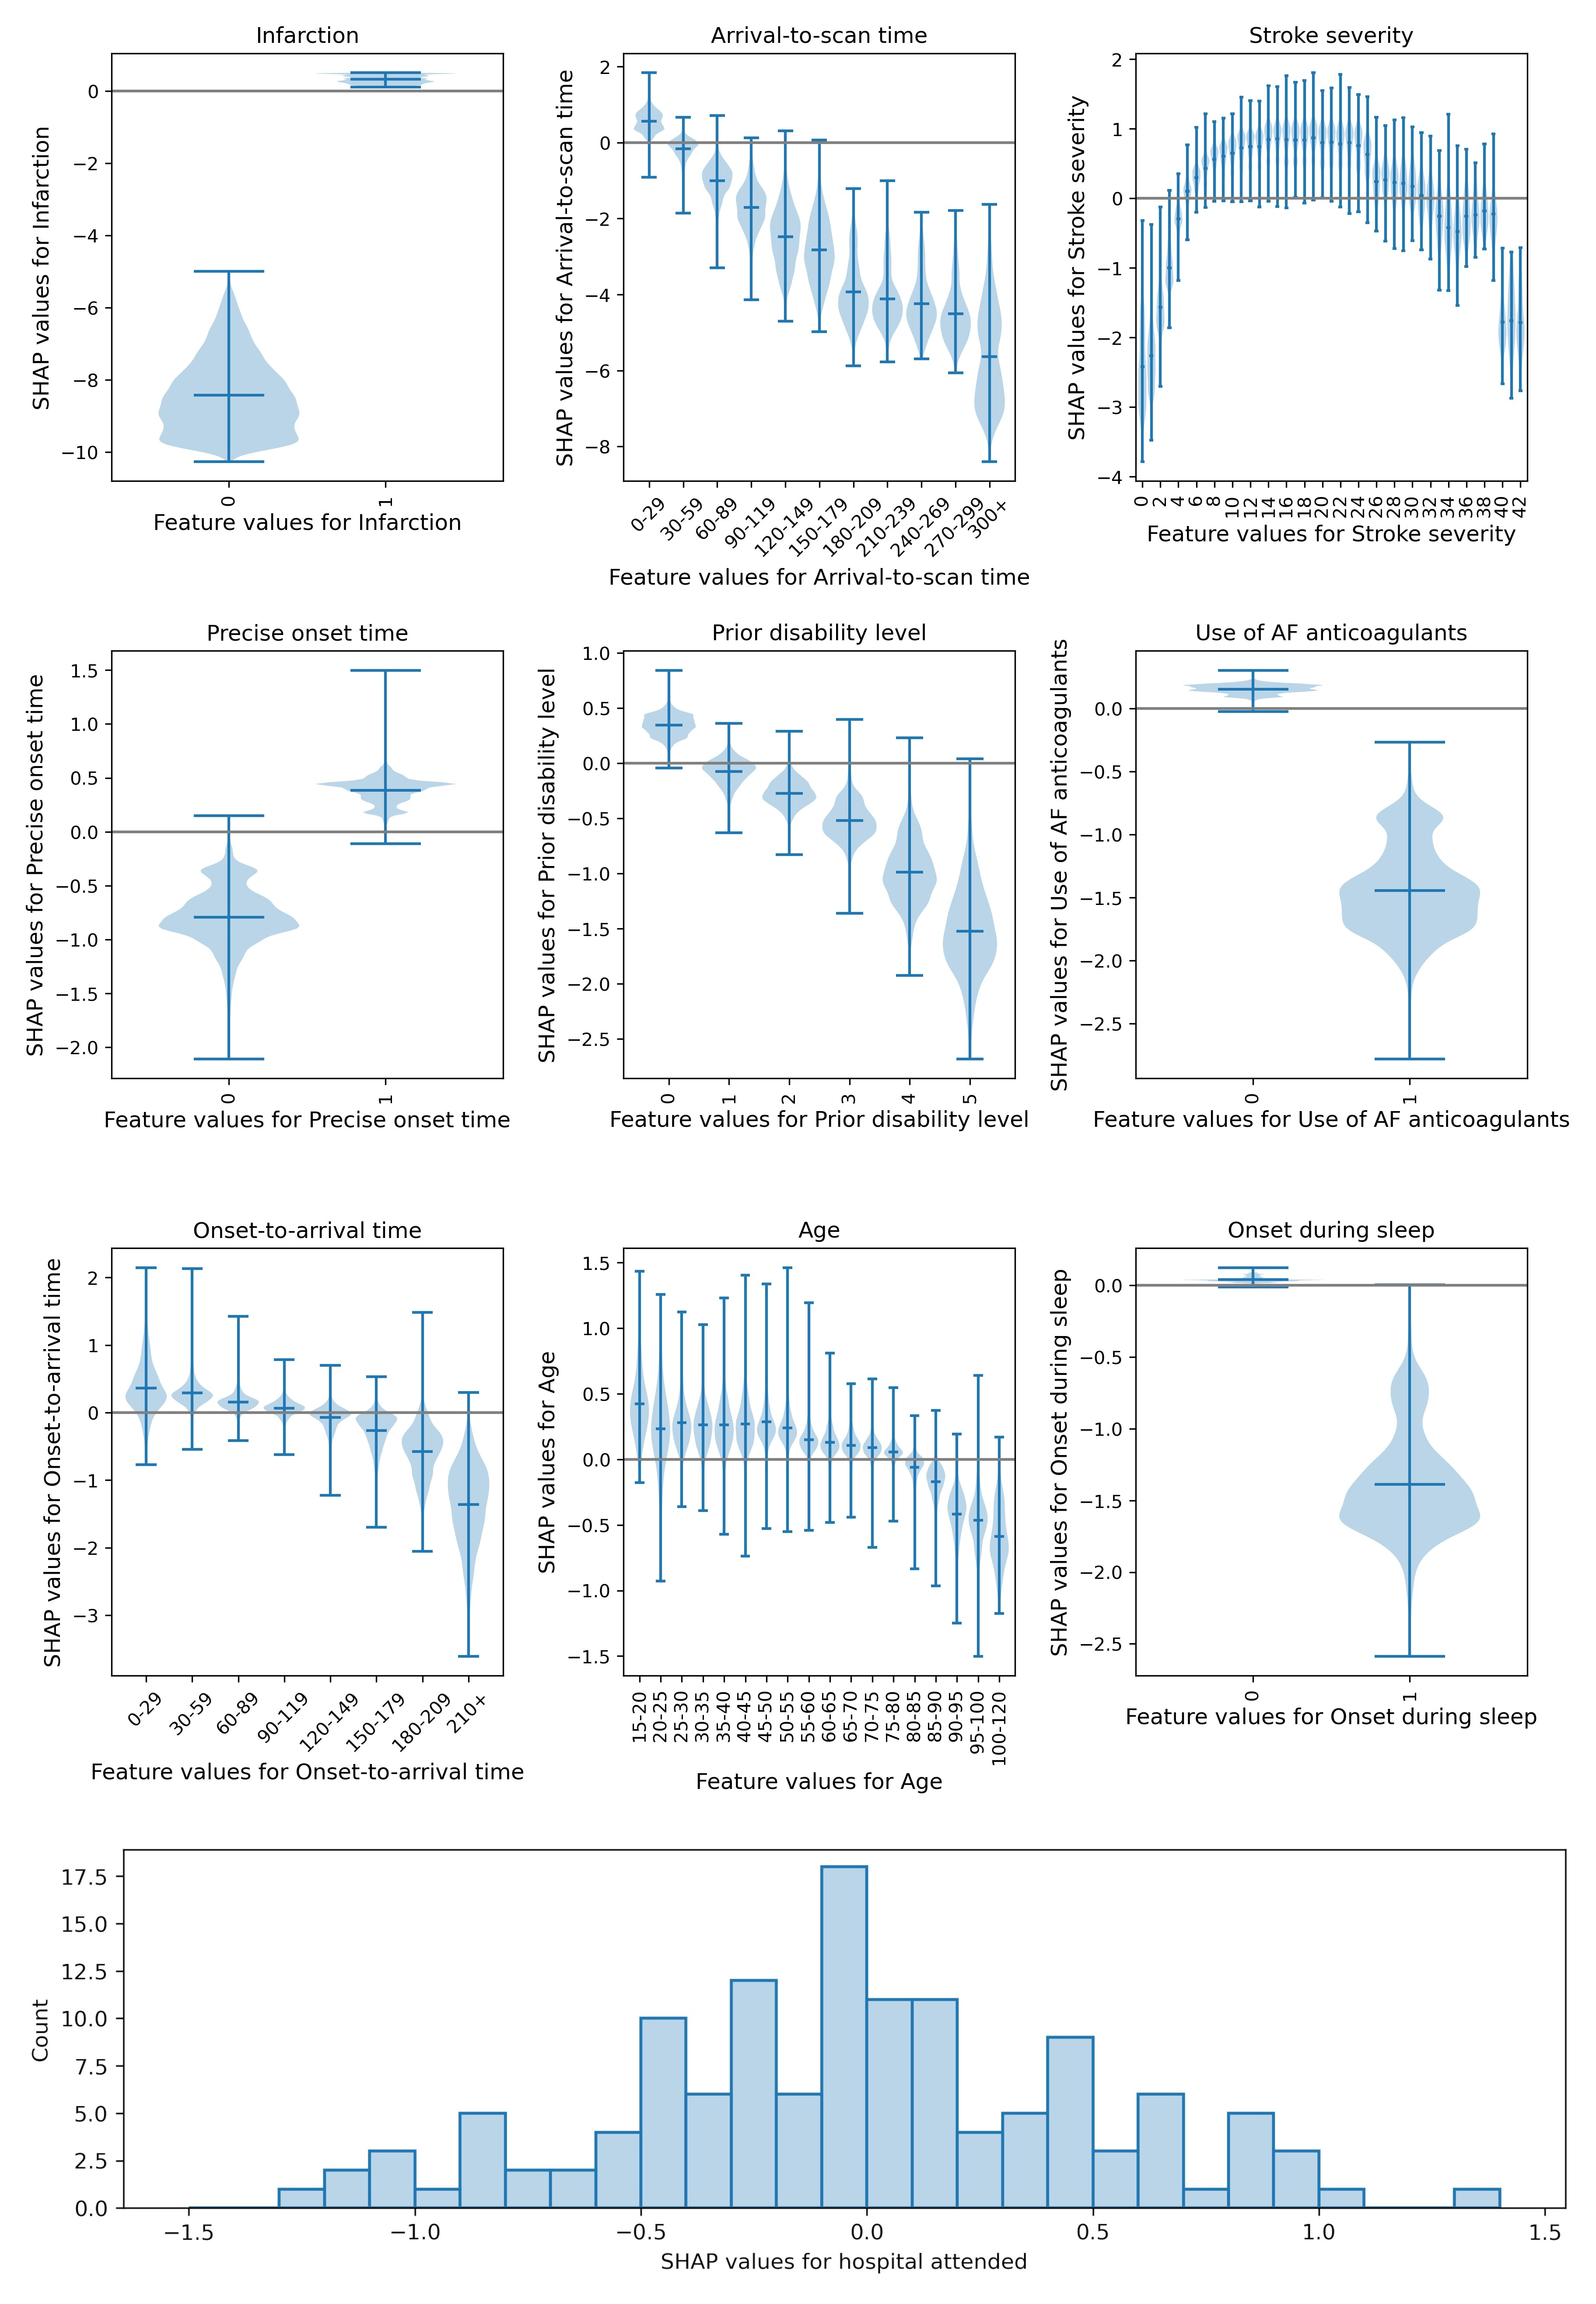
\includegraphics[width=0.9\textwidth]{./images/03a_combined_shap}
\caption{Plots showing the relationship between SHAP values and feature values. Top: Violin plots showing the relationship between SHAP values and feature values. The horizontal line shows the median SHAP value. The plots are ordered in ranked feature importance (using the mean absolute SHAP value across all instances). Bottom: Histogram showing the frequency of SHAP values for the hospital attended.}
\label{fig:shap_feature_subfigure}
\end{figure}

%%%%%%%%%%%%%%%%%%%%%%%%%%%%%%%%%%%%%%%%%%%%%%%%%%%%%%%%%%%%%%%%%%%%%%%%

\subsection{Investigating how the identity of a hospital influences thrombolysis rate}

The mean hospital SHAP main effect value correlated with the observed hospital thrombolysis rate with an r-squared of 0.558 (figure \ref{fig:shap_correlation}, left), suggesting that 56\% (P$<$0.0001) of the between-hospital variance in thrombolysis use may be explained by the attended hospitals' SHAP main effect values, i.e. the hospitals' predisposition and/or preparedness to use thrombolysis.

Using the \emph{10k holdout model}, the predicted use of thrombolysis across the 132 hospitals for the identical 10k cohort of patients ranged from 10\% to 45\%. The mean hospital SHAP main effect value for the 10k cohort correlated very closely with the predicted thrombolysis use in the 10k cohort at each hospital (r-squared of 0.971, figure \ref{fig:shap_correlation}, right), confirming that the hospital SHAP main effect value is providing direct insight into hospitals' propensity to use thrombolysis.

\begin{figure}[!h]
\centering
\begin{subfigure}{.49\textwidth}
  \centering
    \caption*{\footnotesize{\textsf{Observed thrombolysis}}}
    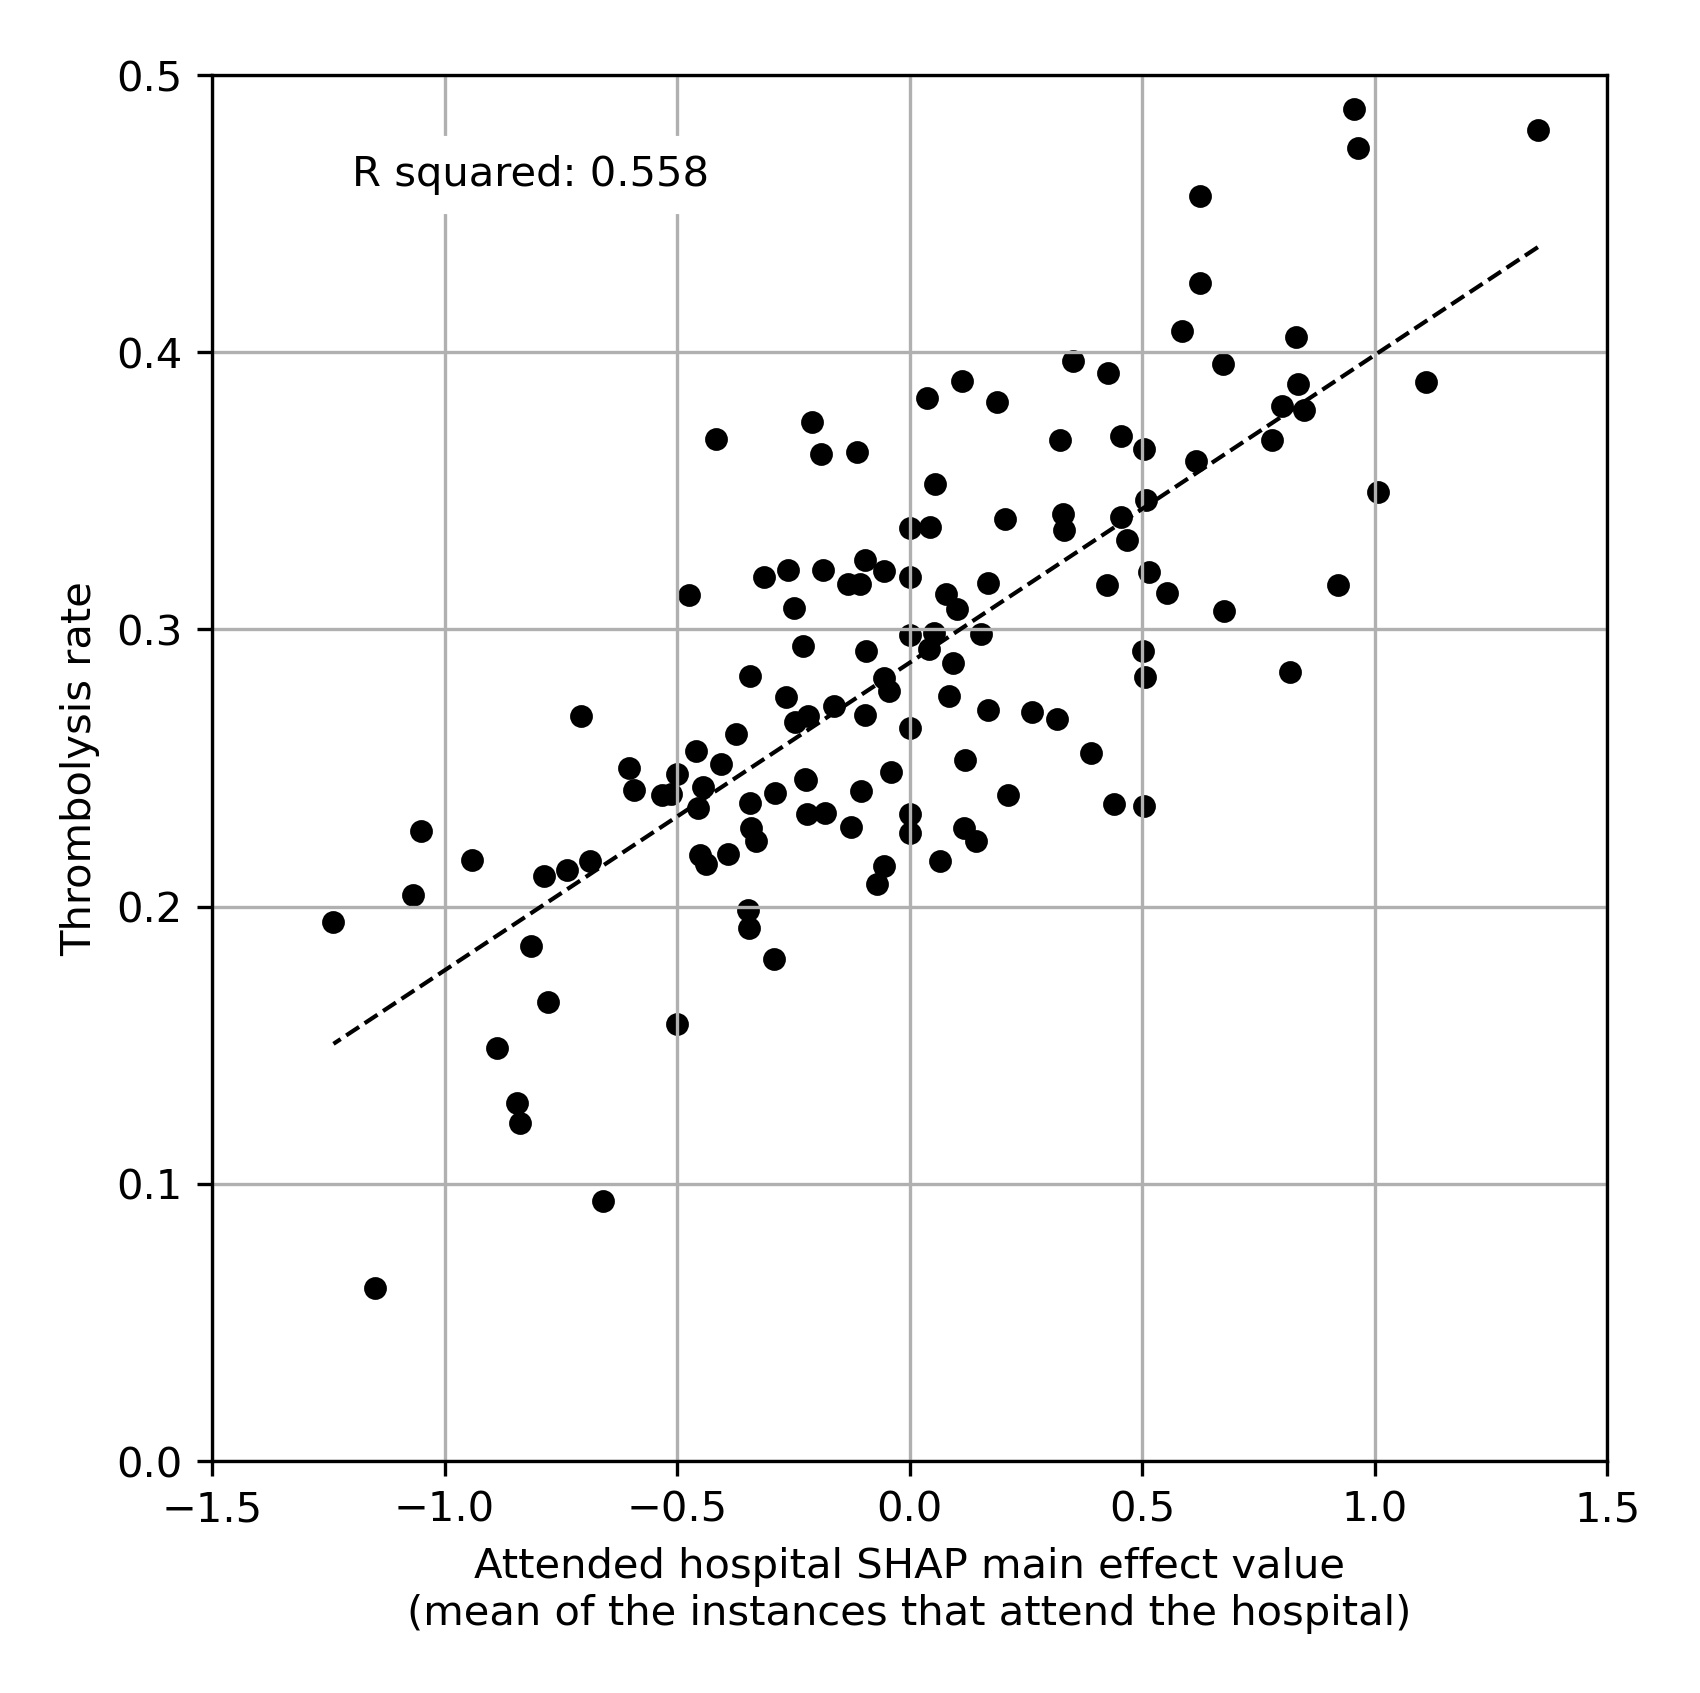
\includegraphics[width=0.9\textwidth]{./images/03c_xgb_10_features_attended_hosp_shap_maineffect_vs_ivt_rate}
\end{subfigure}
\begin{subfigure}{.49\textwidth}
  \centering
    \caption*{\footnotesize{\textsf{Predicted 10K thrombolysis}}}
    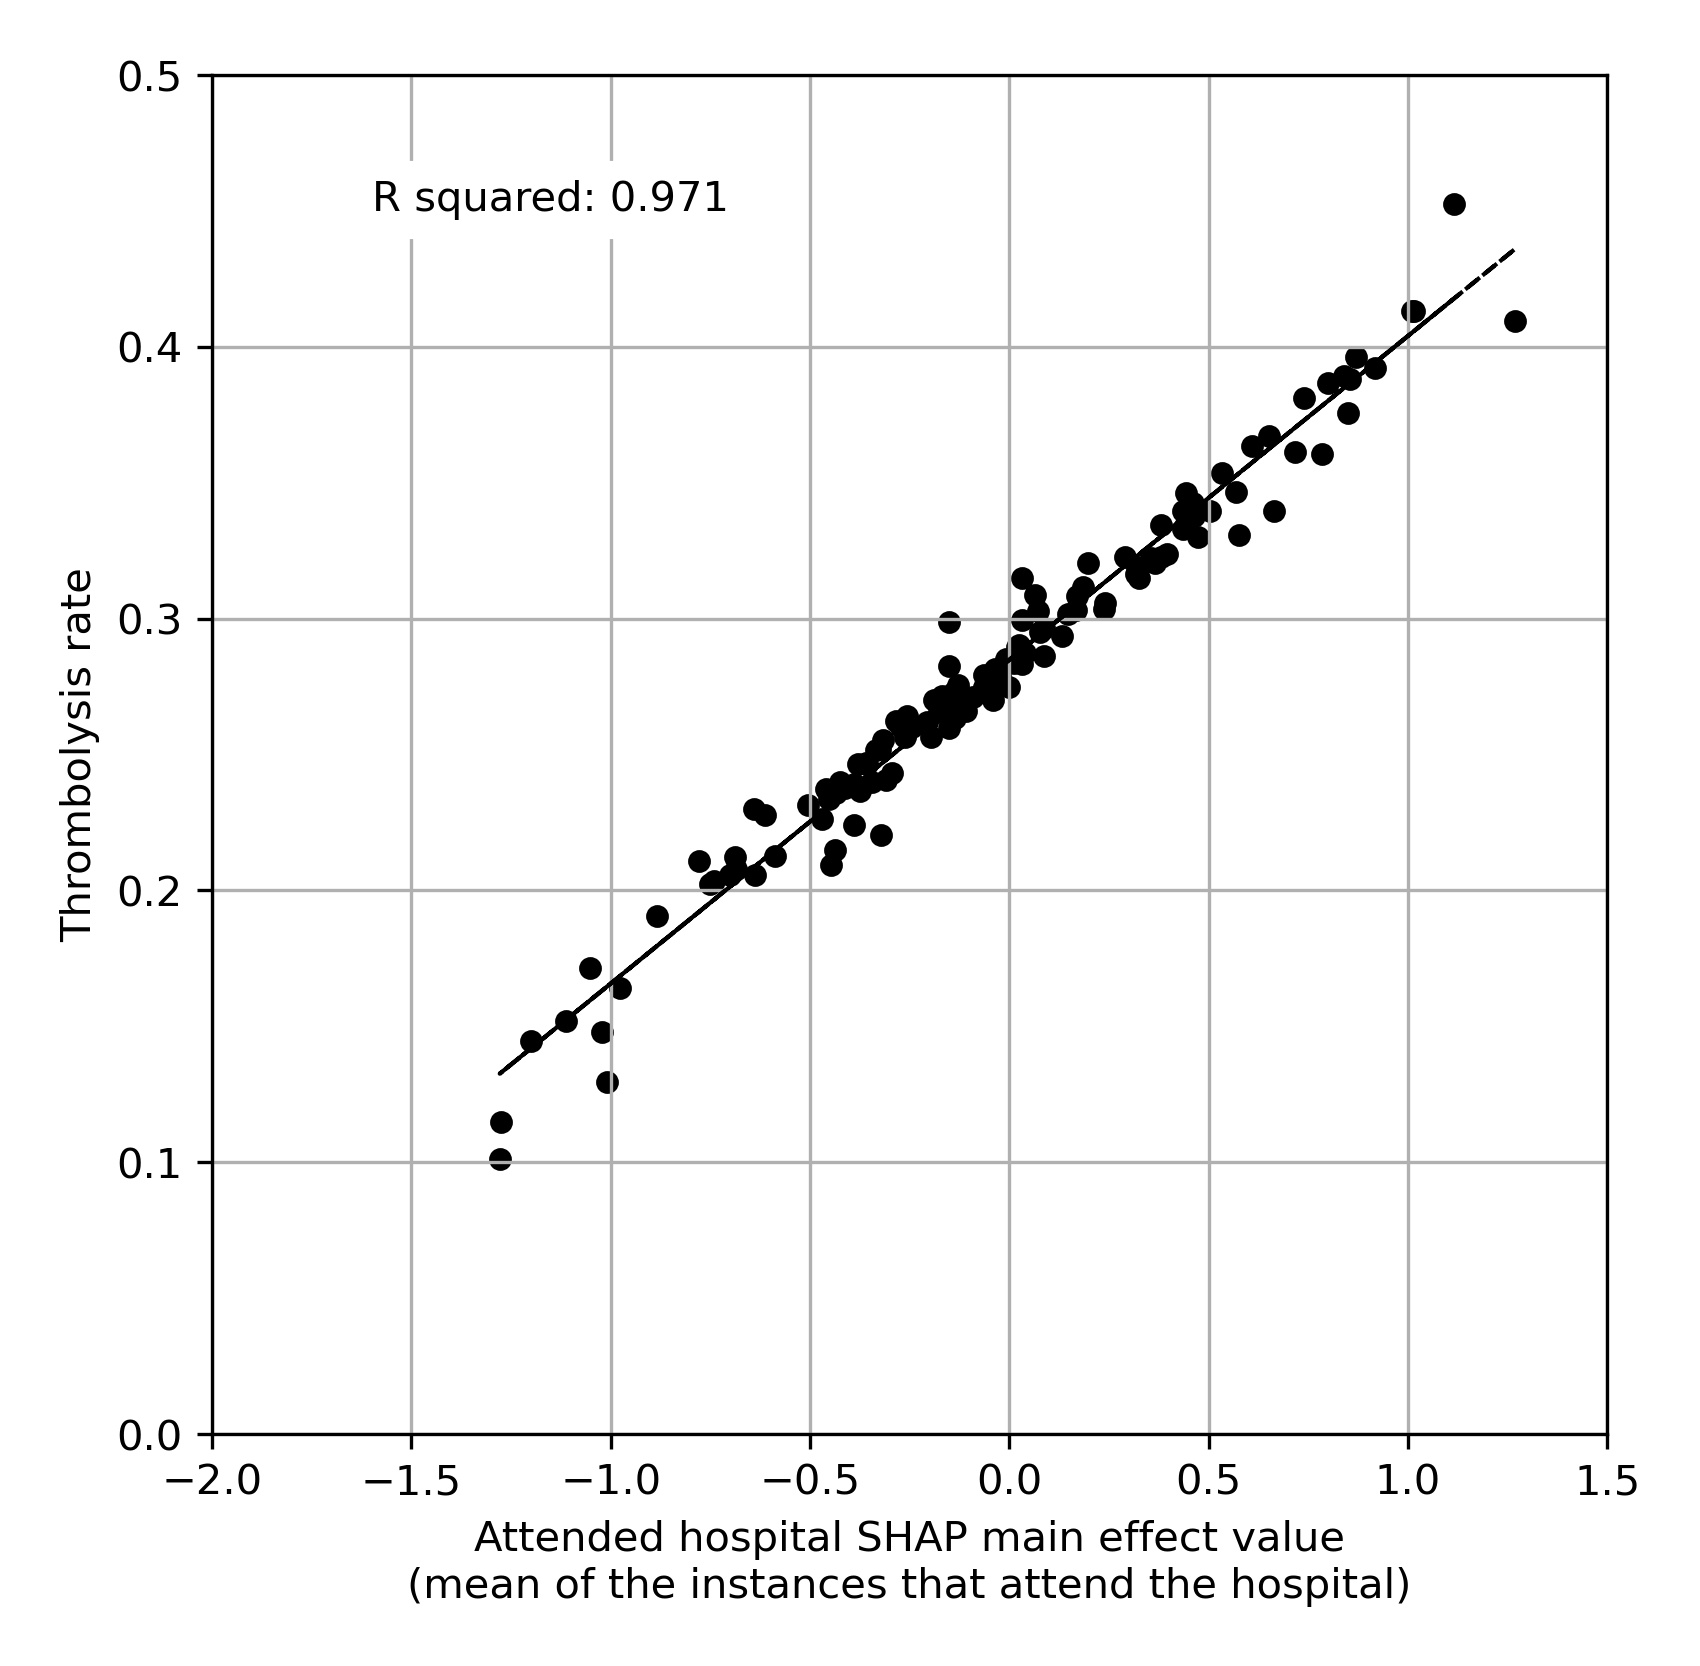
\includegraphics[width=0.9\textwidth]{./images/04a_xgb_10_features_10k_cohort_attended_hosp_shap_maineffect_vs_ivt_rate}
\end{subfigure}

\caption{Correlations between hospital SHAP main effect value and the observed thrombolysis use at each hospital. Left: Observed thrombolysis (using the all data model). Right: Predicted 10k cohort thrombolysis rate.}
\label{fig:shap_correlation}
\end{figure}
%%%%%%%%%%%%%%%%%%%%%%%%%%%%%%%%%%%%%%%%%%%%%%%%%%%%%%%%%%%%%%%%%%%


%\newpage
\subsection{Investigating how patient populations and hospital identity and processes influences thrombolysis rate}

We predicted thrombolysis use using mean subset SHAP values for patients attending each hospital. Figure \ref{fig:shap_multiple_regression} shows that 36\% (P$<$0.0001) of the variance in observed between-hospital thrombolysis use can be explained by the patient population, 74\% (P$<$0.0001) can be explained by hospital identity and processes, and that 95\% (P$<$0.0001) can be explained by the combined information from both the patient population and hospital identity and processes. 

\begin{figure}[!h]
    \centering
    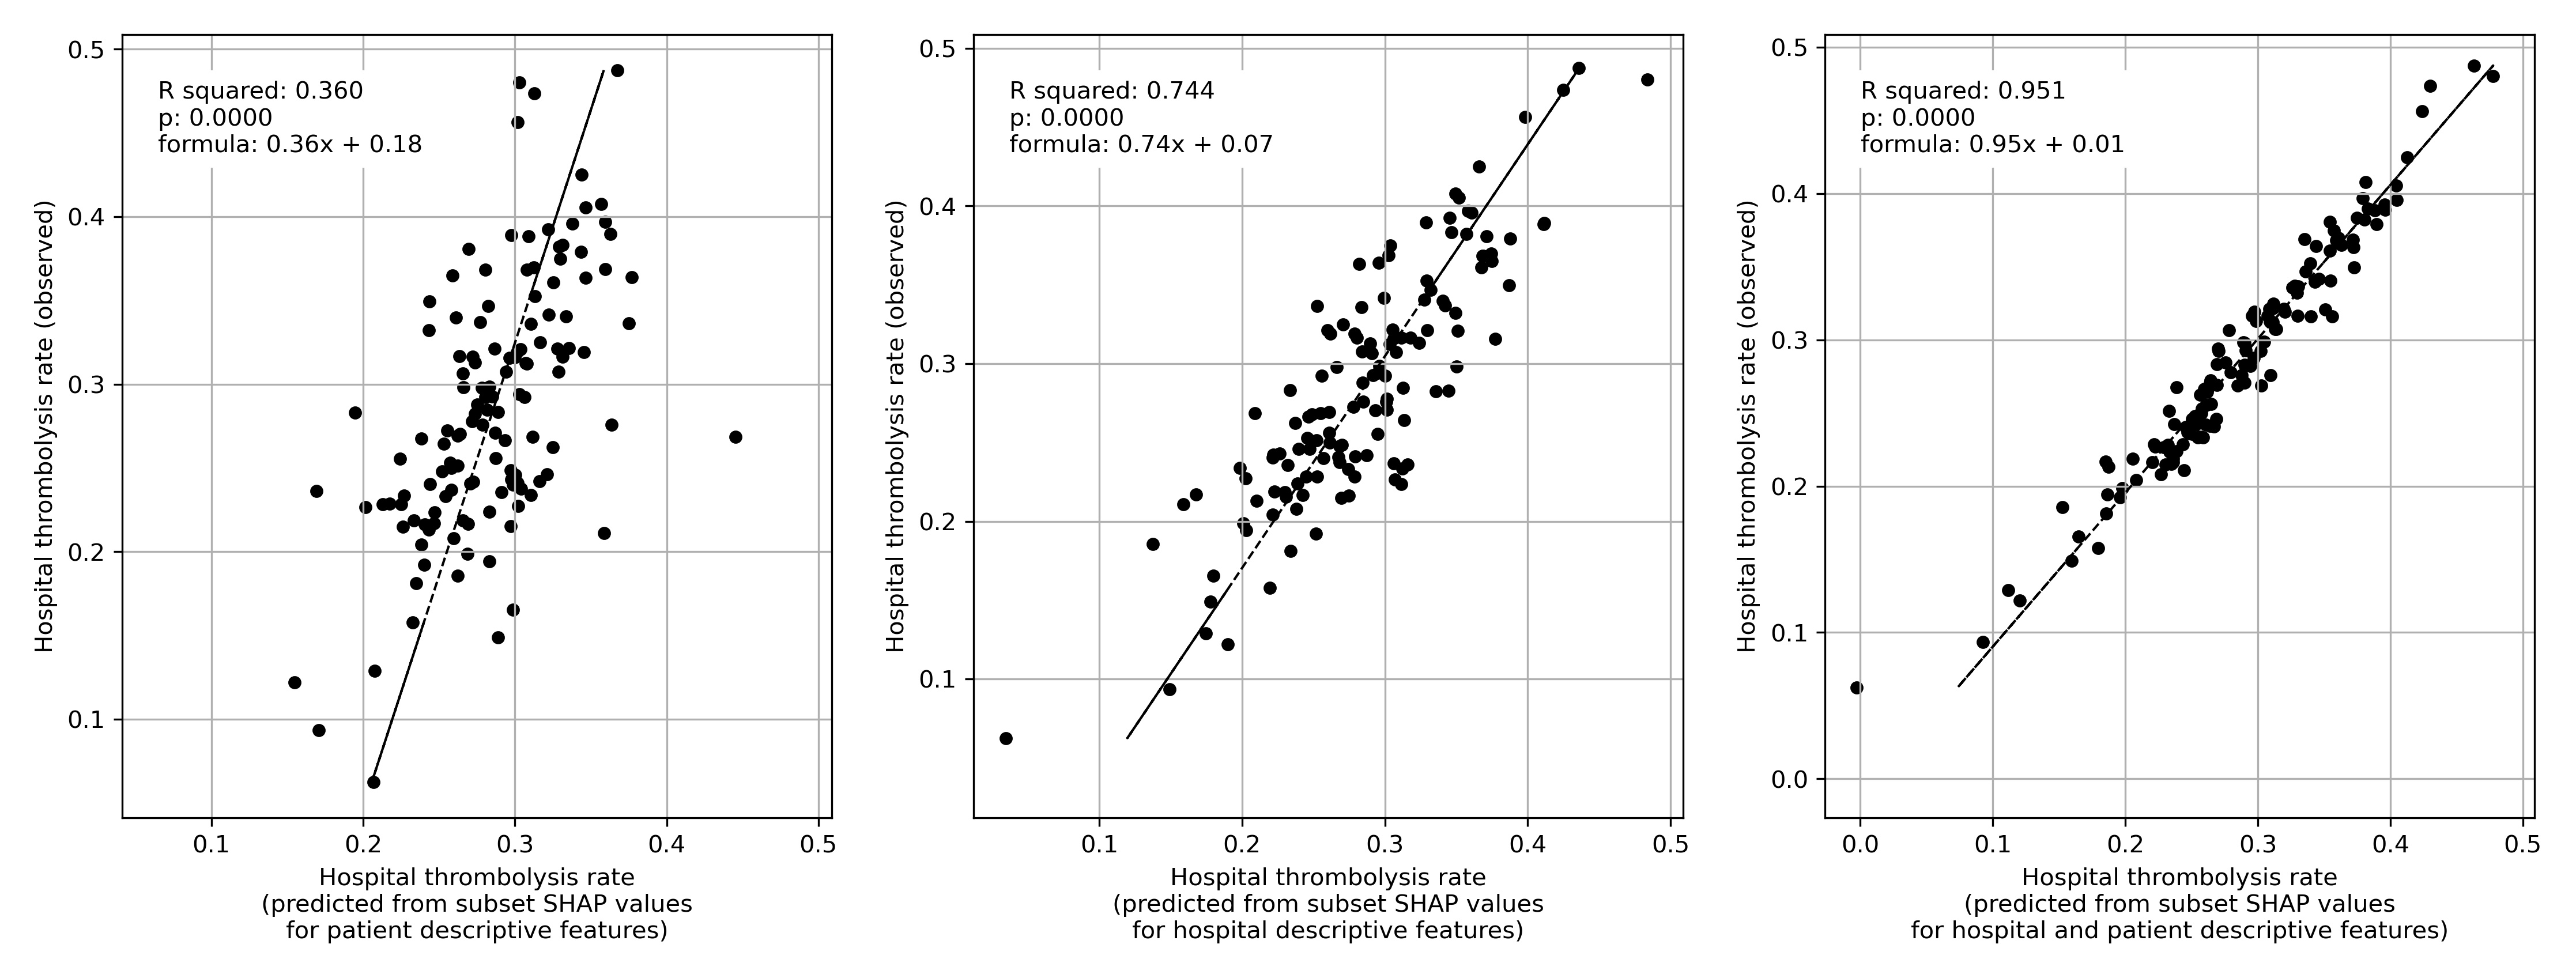
\includegraphics[width=0.9\textwidth]{./images/03f_xgb_10_features_multiple_regression_patient_hospital}
    \caption{Multiple regression of subset SHAP values (mean of patients attending hospital) with hospital observed thrombolysis rate. Left: Subset SHAP values for the eight patient descriptive features (age, stroke severity, prior disability, onset-to-arrival time, stroke type, type of onset time, anticoagulants, and onset during sleep). Middle: Subset SHAP values for the two hospital descriptive features (arrival-to-scan time, and hospital attended). Right: Subset SHAP values for all 10 features (for both hospital and patient descriptive features).}
  \label{fig:shap_multiple_regression}
\end{figure}

%%%%%%%%%%%%%%%%%%%%%%%%%%%%%%%%%%%%%%%%%%%%%%%%%%%%%%%%%%%%%%%%%%%%%%%%
%\newpage
\subsection{Variation in hospital thrombolysis use for patient subgroups}

Figure \ref{fig:results_boxplot} shows observed and predicted use of thrombolysis, broken down by patient subgroup. The subgroups of patients with one defined non-ideal feature all had reduced thrombolysis use than the complete patient population, and combining these non-ideal features reduced thrombolysis use further. There was, however, significant variation between hospitals in use of thrombolysis in each of these subgroups. The observed and predicted thrombolysis use show the same generalpatterns.

\begin{figure}[!h]
\centering
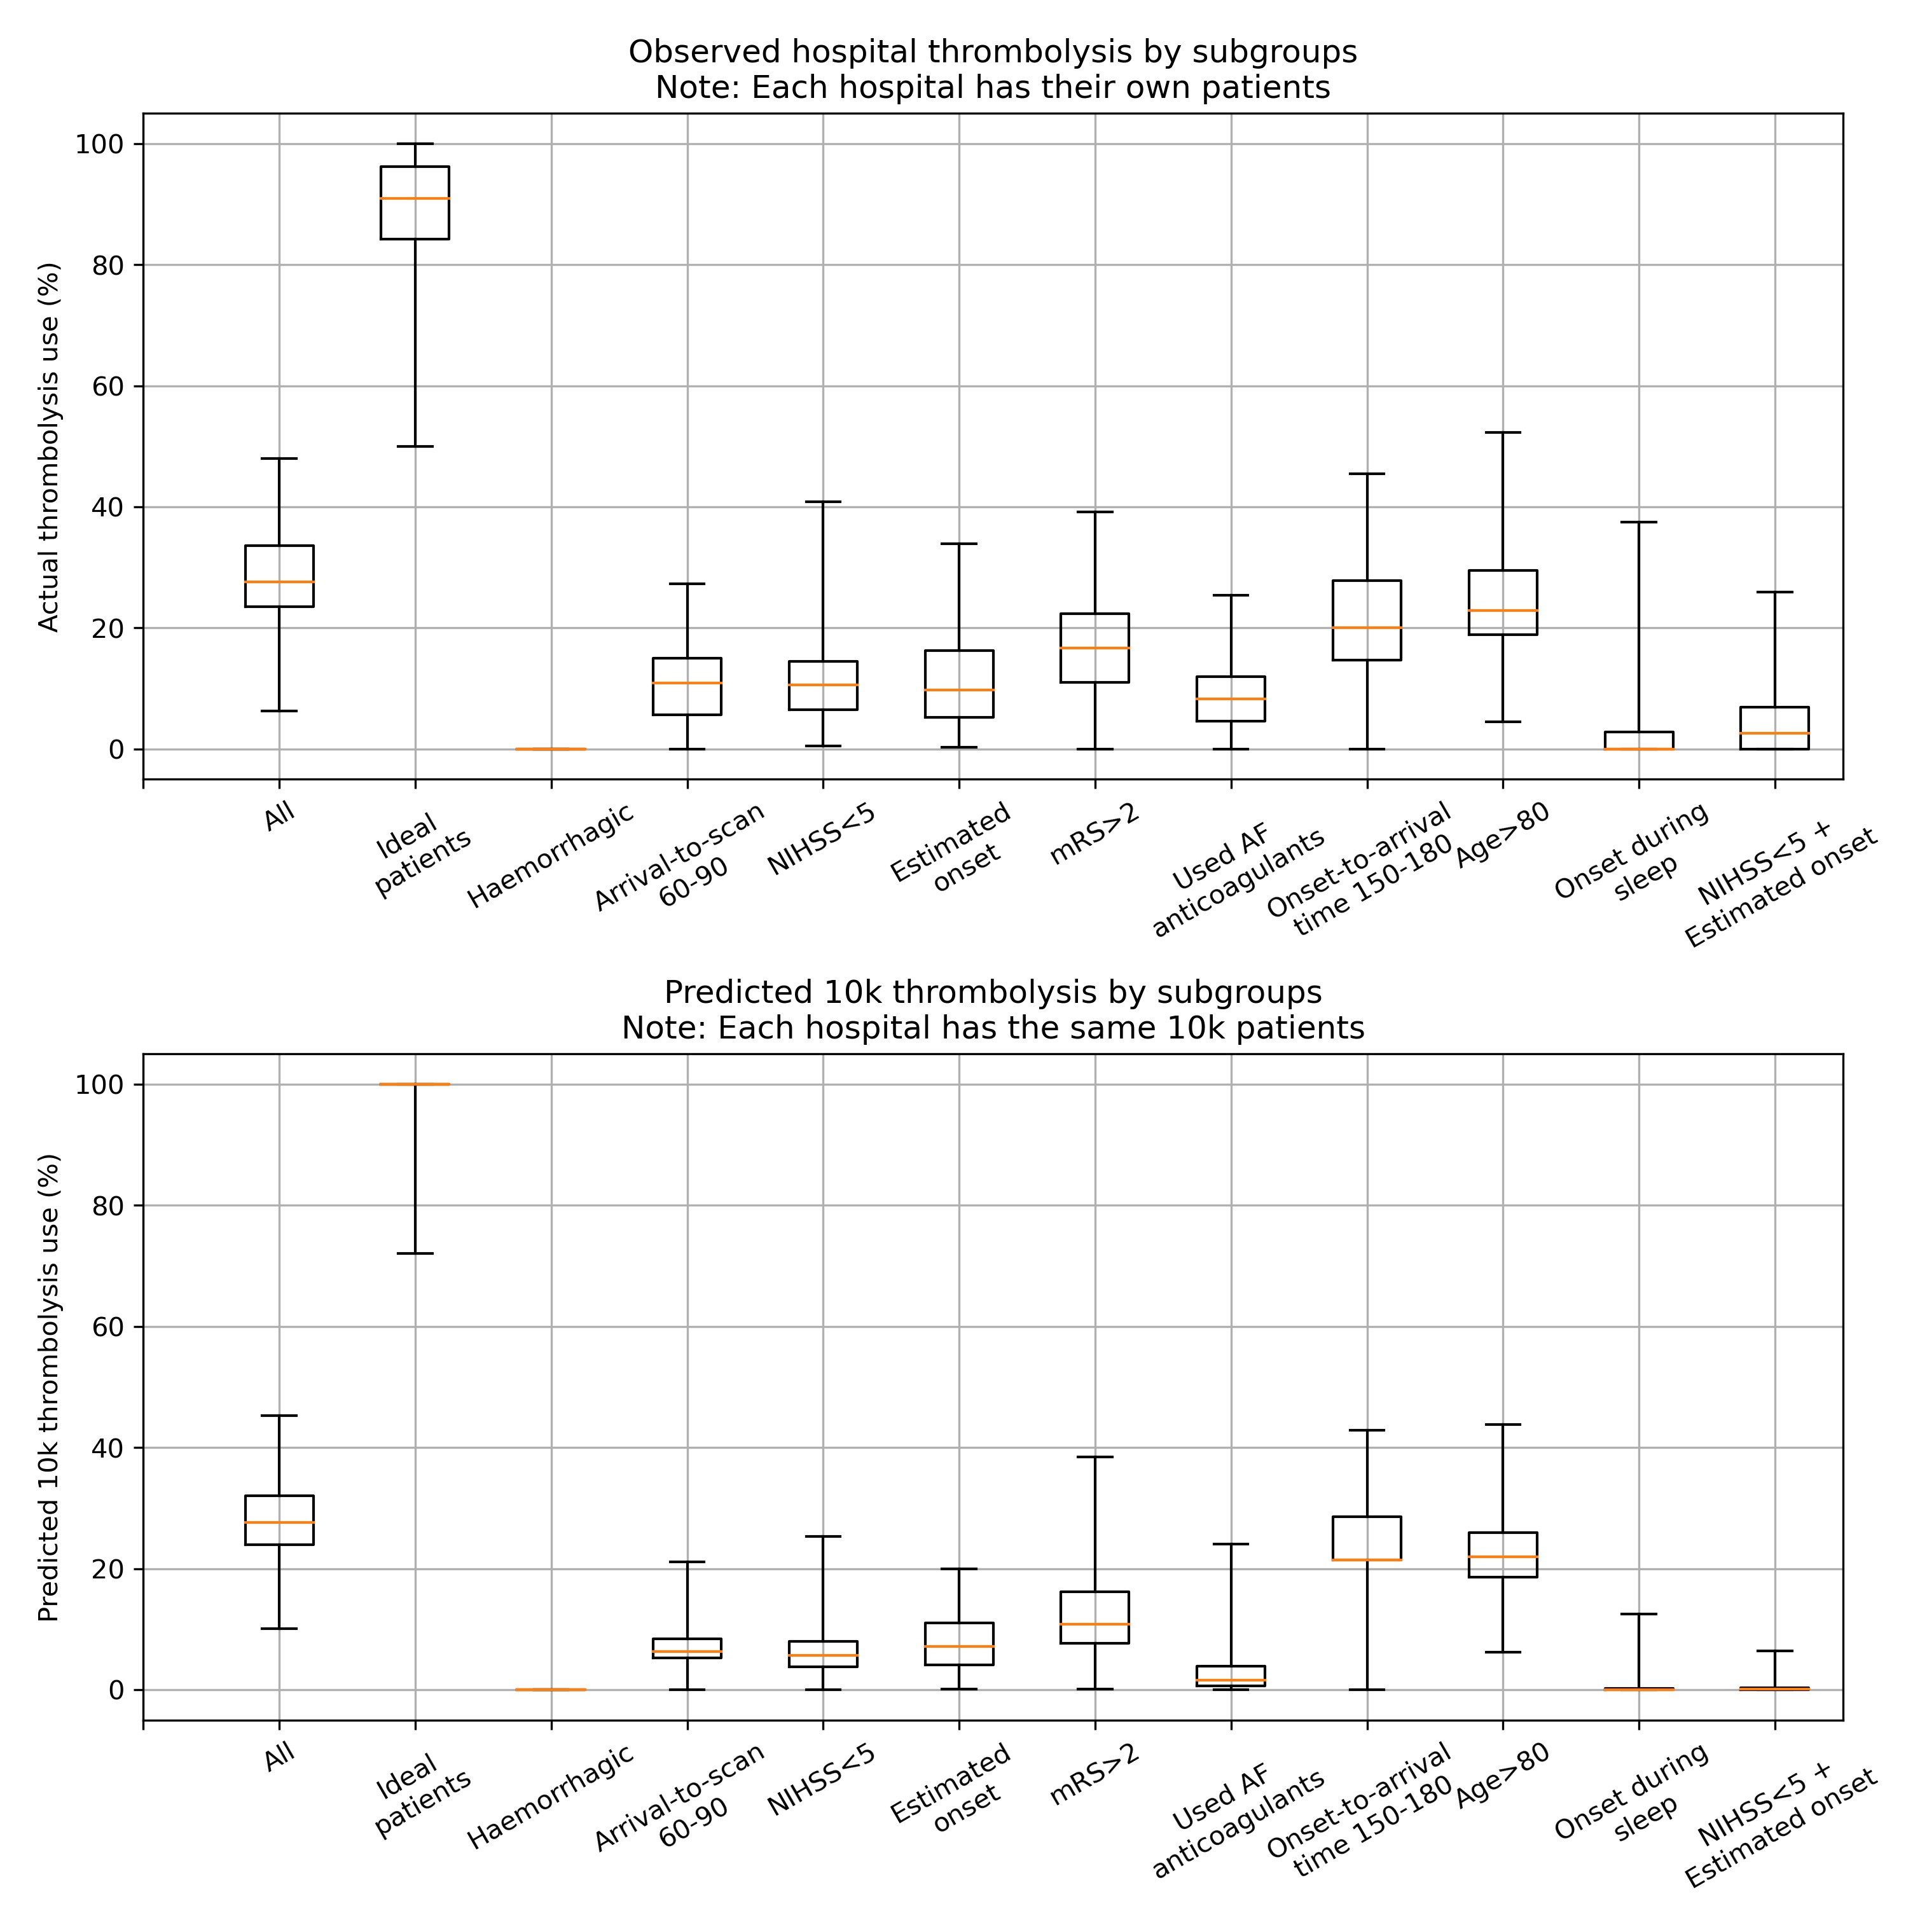
\includegraphics[width=0.75\textwidth]{./images/04c_xgb_10_features_10k_cohort_actual_vs_modelled_subgroup_boxplot}
\caption{Boxplot for either observed (top) or predicted (bottom) use of thrombolysis for subgroups of patients. The `ideal patients' subgroup has a mid-level stroke severity (NIHSS 10-25), short arrival-to-scan time ($<$30 minutes), stroke caused by infarction, precise stroke onset time known, no pre-stroke disability (mRS 0), not taking any atrial fibrillation anticoagulants, short onset-to-arrival time ($<$90 minutes), $<$80 years old, and onset not during sleep. The single features are ordered in ranked feature importance (using the mean absolute SHAP value across all instances).}
\label{fig:results_boxplot}
\end{figure}
\section{Discussion}

We have built on our previous work to predict thrombolysis use from patient level data, by creating an \emph{explainable machine learning model} which maintains the high accuracy that we previously achieved (85\%) \cite{allen_use_2022}. Predicted thrombolysis use at each hospital also very closely matched observed thrombolysis use. The SSNAP registry data used therefore appears to contain most of the information used to make thrombolysis decisions in clinical practice, and can explain the very large majority of between-hospital variation in thrombolysis use.

In general, using SHAP values to uncover the relationship between patient characteristics and the probability of receiving thrombolysis, we found that the probability of receiving thrombolysis fell with increasing arrival-to-scan times, was dependent on stroke severity with the probability of receiving thrombolysis being highest between NIHSS 10 and 25, was lower when onset time was estimated rather than known precisely, and fell with increasing disability prior to stroke. These patterns are similar to the observations of a discrete choice experiment with hypothetical patients \cite{de_brun_factors_2018}, but in our study we confirm these patterns in actual use of thrombolysis, can be quantitative about the effect, and we add the importance of time-to-scan and whether an onset time is known precisely. 

Hospital SHAP values correlated very closely with the predicted use of thrombolysis in a 10k cohort of patients, confirming that the hospital SHAP main effect value provides a measure of the predisposition of a hospital to use thrombolysis. We found that hospital identity and processes explained 74\% of the variance in observed thrombolysis for patients arriving in time to receive thrombolysis.

After observing the general patterns that exist in the use of thrombolysis, we created a subgroup of patients reflecting what appeared to be an \emph{ideal} candidate for thrombolysis, and also a subgroup per feature where we expected to see lower use of thrombolysis. Observed thrombolysis in these groups reflected the patterns identified by the SHAP analysis. For the \emph{ideal} candidates of thrombolysis, half of stroke units would give thrombolysis to at least 90\% of these patients, but some units gave it to significantly fewer patients. Use of thrombolysis in the other subgroups of patients was, as expected, lower, but use also varied significantly between hospitals. Hospitals have different levels of tolerance for non-ideal patient characteristics. These patterns, of lower but varying use, were repeated with expected use of thrombolysis in the same 10k patient cohort of patients.

This novel analysis examines and aids understanding of between-hospital variation in clinical decision making in the acute stroke setting. The use of large datasets such as SSNAP to understand sources of variation in clinical practice between large number of acute stroke centres across the UK presents a unique opportunity to understand the specific influences behind the significant residual between-hospital variation in thrombolysis use. In particular, it allows national quality improvement projects such as SSNAP to counter one of the most common objections raised to comparative audit: that the patients presenting to any one particular site are in some way unique, thereby accounting for most of the variation in clinical quality between that site and all the others. Although the patient population does vary between hospitals, and will contribute to the thrombolysis use achievable by an individual hospital, the majority of between-hospital variation can be explained by hospital-level rather than patient-level factors.

It is disappointing that even though this disability-saving treatment was first licensed for approval for use over 20 years ago, it is still subject to such large variation in clinical judgement or opinion regarding the selection of patients most appropriate for use. In our previous work \cite{allen_using_2022}, we have shown that increasing the uptake of thrombolysis through the administration of treatment to more patients and sooner after stroke, offers the prospect of more than doubling the proportion of patients after stroke who are left with little or no disability (mRS 0 or 1). At a time when there is an appropriate focus of effort on expanding the use of endovascular therapy in acute ischaemic stroke, it is sobering to consider how much population benefit there still remains to accrue from the fullest possible implementation of a cheaper technology that has been available for over 20 years. Far greater scrutiny of such residual variation in clinical practice is clearly warranted, given the extent to which it appears to be acting as a barrier to successful implementation. Recent studies have highlighted that clinicians can be reluctant to modify their behaviour in response to audit and feedback when it is not seen to be clinically meaningful, recent or reliable \cite{bekker_give_2022}, so the full potential of audit and feedback is not realised \cite{foy_revitalising_2020} despite the evidence of a beneficial effect especially when baseline performance is low \cite{ivers_audit_2012}. The development of bespoke, individualised feedback (at least at hospital level) based on actual and recent activity may increase the impact of efforts at data-driven quality improvement targeted at increasing overall uptake of thrombolysis through reducing variation.

\subsection{Limitations}

This machine learning study is necessarily limited to data collected for the national stroke audit. Though we have high accuracy, and can identify clear patterns of use of thrombolysis, the data will not be sufficient to provide a decision-support tool or to review decision-making at an individual patient level. Nor is it a causal model. We may also be missing information that could otherwise have improved the accuracy still further. The model has high accuracy and can identify clear patterns, suggesting the capability to identify and characterise a centre's culture in the use of thrombolysis, but we do not identify variation in thrombolysis between individual clinicians in the same hospital.

We acknowledge that not all countries have a national stroke audit dataset, however we hope that this paper helps to demonstrate what type of analysis can be done should resources be allocated to collect their national data.

%\section{References}
\bibliographystyle{naturemag}
%\bibliographystyle{plainnat}
%\bibliographystyle{unsrt}
%\bibliographystyle{unsrtnat}
\bibliography{references}

% Force new page
\clearpage
\newpage

\subsection*{Acknowledgements}

We would like to thank the SAMueL project team, the Patient and Carer Involvement team, and the expert advisory group, for their input into this work (see appendix for details).

\subsection*{Data access and ethics}

The NHS Health Research Authority decision tool was used to confirm that ethical approval was not required to access the data. No identifiable patient or hospital information were provided in the data, and anonymised hospital names were provided. Governance of the data and access to SSNAP was authorised by the Healthcare Quality Improvement Partnership (HQIP, reference HQIP303). 

\subsection*{Funding}

This research was funded by the National Institute for Health Research Applied Research Collaboration South West Peninsula and by the National Institute for Health Research Health and Social Care Delivery Research (HSDR) Programme [NIHR134326]. The views expressed in this publication are those of the authors and not necessarily those of the National Institute for Health Research or the Department of Health and Social Care.

\subsection*{Author approval}

All authors have seen and approved this manuscript.

\subsection*{Conflict of interest statement}

All authors declare no conflicts of interest.

\subsection*{Links to source code, and online Jupyter book}
\begin{enumerate}
    \item GitHub repository: \url{https://github.com/samuel-book/samuel_shap_paper_1} 
    \item Jupyter book: \url{https://samuel-book.github.io/samuel_shap_paper_1/}
\end{enumerate}

%% Add wordcounts
\newcommand{\detailtexcount}[1]{%
  \immediate\write18{texcount -merge -sum -total -quiet  #1.tex output.bbl > #1.wcdetail }%
  \verbatiminput{#1.wcdetail}%
}

\newcommand{\quickwordcount}[1]{%
  \immediate\write18{texcount -1 -sum -merge -q #1.tex output.bbl > #1-words.sum }%
  \input{#1-words.sum} words%
}

\newcommand{\quickcharcount}[1]{%
  \immediate\write18{texcount -1 -sum -merge -char -q #1.tex output.bbl > #1-chars.sum }%
  \input{#1-chars.sum} characters (not including spaces)%
}

%TC:ignore
\clearpage
\newpage
\subsection*{Wordcount}
%\quickwordcount{main}
%\quickcharcount{main}
\detailtexcount{main}
%TC:endignore

%TC:ignore
%\appendix
\section{Appendix}

% Use numbering specific to the appendix.
\renewcommand{\thefigure}{\thesection.\arabic{figure}}
\renewcommand{\thetable}{\thesection.\arabic{table}}

This work is licensed under a Creative Commons \ccby{3.0} license.

All code, with detailed results, used is available online as a Jupyter book at \url{https://samuel-book.github.io/samuel_shap_paper_1/} and available on GitHub at \url{https://github.com/samuel-book/samuel_shap_paper}

\subsection{Data}

\subsubsection{Data access}

Data was obtained from the Sentinel Stroke National Audit (SSNAP\footnote{https://www.strokeaudit.org/}), managed through the Healthcare Quality Improvement Partnership (HQIP\footnote{https://www.hqip.org.uk/}). SSNAP has near-complete coverage of all acute stroke admissions in the UK (outside Scotland). All hospitals admitting acute stroke participate in the audit, and year-on-year comparison with Hospital Episode Statistics\footnote{https://digital.nhs.uk/data-and-information/data-tools-and-services/data-services/hospital-episode-statistics} confirms estimated case ascertainment of 95\% of coded cases of acute stroke.

The NHS Health Research Authority decision tool\footnote{http://www.hra-decisiontools.org.uk/research/} was used to confirm that ethical approval was not required to access the data. Data access was authorised by HQIP (reference HQIP303). 

Data were retrieved for 246,676 emergency stroke admissions to acute stroke teams in England and Wales for the three calendar years 2016 - 2018, obtained from the Sentinel Stroke National Audit Programme\footnote{https://www.strokeaudit.org/} (SSNAP). Data fields were provided for the hyper-acute phase of the stroke pathway, up to and including our target feature: \emph{receive thrombolysis} (full details of the data fields obtained are provided in the appendix). Of these patients, 88,928 arrived within 4 hours of known (precise or estimated) stroke onset, and were used in this modelling study. The data included 132 acute stroke hospitals (these were all units admitting an average of 100 patients per year, and delivering thrombolysis to at least 10 patients over 3 years). There are 60 original features used from the SSNAP dataset.

 SSNAP has near-complete coverage of all acute stroke admissions in the UK (outside Scotland). All hospitals admitting acute stroke participate in the audit, and year-on-year comparison with Hospital Episode Statistics\footnote{https://digital.nhs.uk/data-and-information/data-tools-and-services/data-services/hospital-episode-statistics} confirms estimated case ascertainment of 95\% of coded cases of acute stroke.

\subsubsection{Data fields}

\paragraph{Stroke Team}

\begin{itemize}
\item \emph{StrokeTeam}: Pseudonymised SSNAP `routinely admitting team` unique
  identifier. For emergency care it is expected that each hospital has
  one stroke team (though post-72 hour care may be reported under a
  different team at that hospital).
\end{itemize}

\paragraph{Patient -- general}

\begin{itemize}
\item  \emph{Pathway}: Total number of team transfers, excluding community teams
\item \emph{S1AgeOnArrival}: Age on arrival aggregated to 5 year bands
\item \emph{MoreEqual80y}: Whether the patient is \textgreater= 80 years old at the
  moment of the stroke
\item \emph{S1Gender}: Gender
\item \emph{S1Ethnicity}: Patient Ethnicity. Aggregated to White, Black, Mixed,
  Asian and Other
\end{itemize}


\paragraph{Patient -- pathway information}

\begin{itemize}
\item \emph{S1OnsetInHospital}: Whether the patient was already an inpatient at the
  time of stroke
\item \emph{S1OnsetToArrival\_min}: Time from symptom onset to arrival at hospital
  in minutes, where known and if out of hospital stroke
\item \emph{S1OnsetDateType}: Whether the date of onset given is precise, best
  estimate or if the stroke occurred while sleep
\item \emph{S1OnsetTimeType}: Whether the time of symptom onset given is precise,
  best estimate, not known
\item \emph{S1ArriveByAmbulance}: Whether the patient arrived by ambulance
\item \emph{S1AdmissionHour}: Hour of arrival, aggregates to 3 hour epochs
\item \emph{S1AdmissionDay}: Day of week at the moment of admission
\item \emph{S1AdmissionQuarter}: Year quarter (Q1: Jan-Mar; Q2:April-Jun; Q3:
  Jul-Sept; Q4: Oct-Dec)
\item \emph{S1AdmissionYear}: Year of admission
\item \emph{S2BrainImagingTime\_min}: Time from Clock Start to brain scan. In
  minutes. ``Clock Start'' is used throughout SSNAP reporting to refer
  to the date and time of arrival at first hospital for newly arrived
  patients, or to the date and time of symptom onset if patient already
  in hospital at the time of their stroke.
\item \emph{S2ThrombolysisTime\_min}: Time from Clock Start to thrombolysis. In
  minutes. ``Clock Start'' is used throughout SSNAP reporting to refer
  to the date and time of arrival at first hospital for newly arrived
  patients, or to the date and time of symptom onset if patient already
  in hospital at the time of their stroke.
\end{itemize}

\paragraph{Patient -- comorbidities}

\begin{itemize}
\item \emph{CongestiveHeartFailure}: Pre-Stroke Congestive Heart Failure
\item \emph{Hypertension}: Pre-Stroke Systemic Hypertension
\item \emph{AtrialFibrillation}: Pre-Stroke Atrial Fibrillation (persistent,
  permanent, or paroxysmal)
\item \emph{Diabetes}: Comorbidities: Pre-Stroke Diabetes Mellitus
\item \emph{StrokeTIA}: Pre-Stroke history of stroke or Transient Ischaemic Attack
  (TIA)
\item \emph{AFAntiplatelet}: Only available if ``Yes'' to Atrial Fibrillation
  comorbidity. Whether the patient was on antiplatelet medication prior
  to admission
\item \emph{AFAnticoagulent}: Prior to 01-Dec-2017: Only available if ``Yes'' to
  Atrial Fibrillation comorbidity; From 01-Dec-2017: available even if
  patient is not in Atrial Fibrillation prior to admission. Whether the
  patient was on anticoagulant medication prior to admission
\item \emph{AFAnticoagulentVitK}: If the patient was receiving anticoagulant
  medication, was it vitamin K antagonists
\item \emph{AFAnticoagulentDOAC}: If the patient was receiving anticoagulant
  medication, was it direct oral anticoagulants (DOACs)
\item \emph{AFAnticoagulentHeparin}: If the patient was receiving anticoagulant
  medication, was it Heparin
\end{itemize}

\paragraph{Patient -- NIH Stroke Scale}

\begin{itemize}
\item \emph{S2NihssArrival}: National Institutes of Health Stroke Scale score on
  arrival at hospital
\item \emph{BestGaze}: National Institutes of Health Stroke Scale Item 2 Best Gaze
  (higher values indicate more severe deficit)
\item \emph{BestLanguage}: National Institutes of Health Stroke Scale Item 9 Best
  Language (higher values indicate more severe deficit)
\item \emph{Dysarthria}: National Institutes of Health Stroke Scale Item 10
  Dysarthria (higher values indicate more severe deficit)
\item \emph{ExtinctionInattention}: National Institutes of Health Stroke Scale Item
  11 Extinction and Inattention (higher values indicate more severe
  deficit)
\item \emph{FacialPalsy}: National Institutes of Health Stroke Scale Item 4 Facial
  Paresis (higher values indicate more severe deficit)
\item \emph{LimbAtaxia}: National Institutes of Health Stroke Scale Item 7 Limb
  Ataxia (higher values indicate more severe deficit)
\item \emph{Loc}: National Institutes of Health Stroke Scale Item 1a Level of
  Consciousness (higher values indicate more severe deficit)
\item \emph{LocCommands}: National Institutes of Health Stroke Scale Item 1c Level
  of Consciousness Commands (higher values indicate more severe deficit)
\item \emph{LocQuestions}: National Institutes of Health Stroke Scale Item 1b Level
  of Consciousness Questions (higher values indicate more severe
  deficit)
\item \emph{MotorArmLeft}: National Institutes of Health Stroke Scale Item 5a Motor
  Arm - Left (higher values indicate more severe deficit)
\item \emph{MotorArmRight}: National Institutes of Health Stroke Scale Item 5b
  Motor Arm - Right (higher values indicate more severe deficit)
\item \emph{MotorLegLeft}: National Institutes of Health Stroke Scale Item 6a Motor
  Leg - Left (higher values indicate more severe deficit)
\item \emph{MotorLegRight}: National Institutes of Health Stroke Scale Item 6b
  Motor Leg - Right (higher values indicate more severe deficit)
\item \emph{Sensory}: National Institutes of Health Stroke Scale Item 8 Sensory
  (higher values indicate more severe deficit)
\item \emph{Visual}: National Institutes of Health Stroke Scale Item 3 Visual
  Fields (higher values indicate more severe deficit)
\end{itemize}

\paragraph{Patient -- other clinical features}

\begin{itemize}
\item \emph{S2INR}: Patient's International Normalised ratio (INR) on arrival at
  hospital (available since 01-Dec-2017)
\item \emph{S2INRHigh}: INR was greater than 10 on arrival at hospital (available
  since 01-Dec-2017)
\item \emph{S2INRNK}: INR not checked (available since 01-Dec-2017)
\item \emph{S2NewAFDiagnosis}: Whether a new diagnosis of Atrial Fibrillation was
  made on admission
\item \emph{S2RankinBeforeStroke}: Patient's modified Rankin Scale score before
  this stroke (Higher values indicate more disability)
\item \emph{S2StrokeType}: Whether the stroke type was infarction or primary
  intracerebral haemorrhage
\item \emph{S2TIAInLastMonth}: Whether the patient had a Transient Ischaemic Attack
  during the last month. Item from the SSNAP comprehensive dataset
  questions (not mandatory)
\end{itemize}

\paragraph{Patient -- thrombolysis given}

\begin{itemize}
\item \emph{S2Thrombolysis}: Whether the patient was given thrombolysis (clot
  busting medication)
\end{itemize}

\paragraph{Patient -- reason stated for not giving thrombolysis}

\begin{itemize}
\item \emph{Age}: If the answer to thrombolysis given was ``no but'', the reason
  was Age
\item \emph{Comorbidity}: If the answer to thrombolysis given was ``no but'', the
  reason was Co-morbidity
\item \emph{Haemorrhagic}: If the answer to thrombolysis given was ``no but'', the
  reason was Haemorrhagic stroke
\item \emph{Improving}: If the answer to thrombolysis given was ``no but'', the
  reason was Symptoms Improving
\item \emph{Medication}: If the answer to thrombolysis given was ``no but'', the
  reason was Medication
\item \emph{OtherMedical}: If the answer to thrombolysis given was ``no but'', the
  reason was Other medical reason
\item \emph{Refusal}: If the answer to thrombolysis given was ``no but'', the
  reason was Refusal
\item \emph{TimeUnknownWakeUp}: If the answer to thrombolysis given was ``no but'',
  the reason was Symptom onset time unknown/wake-up stroke
\item \emph{TimeWindow}: If the answer to thrombolysis given was ``no but'', the
  reason was Age
\item \emph{TooMildSevere}: If the answer to thrombolysis given was ``no but'', the
  reason was Stroke too mild or too severe
\end{itemize}

%%%%%%%%%%%%%%%%%%%%%%%%%%%%%%%%%%%%%%%%%%%%%%%%%%%%%%%%%%%%%%%%%%%%%%%%%%%

\subsection{Probability, odds, and Shap values (log odds shifts): A brief explanation}

Many of us find it easiest to think of the chance of something occurring
as a probability. For example, there might be a probability of 10\% that
it will rain today. That is the same as saying there will be one rainy
day out of ten days for days with this given probability of rain.

In our stroke thrombolysis model, Shap values tell us how knowing
something particular about a patient (such as the patient
\emph{feature}, `Is their stroke caused by a clot or a bleed?') adjusts
our prediction of whether they will receive thrombolysis or not.

This is made a little more complicated for us because Shap is usually
reported as a \emph{log odds shift}. It is useful for us to see how
those relate to probabilities, and get a sense of how significant Shap
values in the range of 0.5 to 5 (or -0.5 to -5) are, as that is a common
range of Shap values that we will see in our models.

\subsubsection{Probability}

We will take the example that Shap reports that a model's base
probability prediction, before consideration of features is 0.25, or
a 25\% probability of receiving thrombolysis; that is 1 in 4 patients
with this prediction would be expected to receive thrombolysis.

\subsubsection{Odds}

\emph{Probability} expresses the chance of something happening as the
number of positive occurrences as a fraction of all occurrences
(i.e. the number of patients receiving thrombolysis as a fraction of the
total number of patients).

\emph{Odds} express the chance of something happening as the ratio of
the number of positive occurrences (i.e. receiving thrombolysis) to the
number of negative occurrences (i.e. \emph{not} receiving thrombolysis).

If we have probability prediction of 0.25 would receive thrombolysis,
that would mean 1 in 4 of those patients receive thrombolysis. Expressed
as odds, for every one patient that receives thrombolysis, three will
not. The odds are expressed as 1:3 or 1/3. This may also be calculated
as a decimal (1 divided by 3), 0.333.

Odds (O) and probability (P) may be converted with the following
equations:

\begin{enumerate}
\def\labelenumi{(\arabic{enumi})}
\item
  O = P / (1 - P)
\item
  P = O / (1 + O)
\end{enumerate}

\subsubsection{Shap values: Log odds shifts}

Here we will calculate the effect of Shap values, and try and build some
intuition on the size of effect Shap values of 0.5 to 5 give (we will
look at positive and negative Shap values).

Shap usually outputs the effect of a particular feature in how much it
shifts the odds. For reasons we will not go into here, that shift (which
is the `Shap value') is usually given in `log odds' (the logarithm of
the odds value). For the mathematically inclined, we use the natural log
(\emph{ln}).

Let's look at some Shap values (log odds) and see how much they change
the odds of receiving thrombolysis.

First we'll look at the shift in odds the Shap values give. This is
calculated as \emph{shift = exp(Shap)} (table \ref{tab:odds_1}).

\begin{minipage}{\textwidth}
\begin{longtable}[]{@{}ll@{}}
\caption{The relationship between \emph{odds} and \emph{log odds}.}\\
\toprule
SHAP (log odds) & Shift in odds (multiply original odds)\tabularnewline
\midrule
\endhead
0.5 & 1.65\tabularnewline
1 & 2.72\tabularnewline
2 & 7.39\tabularnewline
3 & 20.1\tabularnewline
4 & 54.6\tabularnewline
5 & 148\tabularnewline
\bottomrule
\label{tab:odds_1}
\end{longtable}
\end{minipage}

\emph{Positive Shap values: a worked example}

Now let us work through an example of starting with a known baseline
\emph{probability} (before we consider what we know about a particular
patient feature), converting that to \emph{odds}, applying a Shap
\emph{log odds shift} for that particular feature, and converting back
to \emph{probability} after we have applied the influence of that
feature.

The the effects of those shifts on our baseline probability of 0.25 are shown in table \ref{tab:odds_2}.

\begin{minipage}{\textwidth}
\begin{longtable}[]{@{}llllll@{}}
\caption{The effect of SHAP values between 0.5 and 5 on a base probability of 0.25}\\
\toprule
Starting P & Starting O & SHAP & Shift (multiply O) & Shifted O &
Shifted P (\%)\tabularnewline
\midrule
\endhead
0.25 (25\%) & 0.333 & 0.5 & 1.65 & 0.550 & 0.3547
(35.5\%)\tabularnewline
0.25 (25\%) & 0.333 & 1 & 2.72 & 0.907 & 0.4754 (47.5\%)\tabularnewline
0.25 (25\%) & 0.333 & 2 & 7.39 & 2.46 & 0.7112 (71.1\%)\tabularnewline
0.25 (25\%) & 0.333 & 3 & 20.1 & 6.70 & 0.8700 (87.0\%)\tabularnewline
0.25 (25\%) & 0.333 & 4 & 54.6 & 18.2 & 0.9479 (94.8\%)\tabularnewline
0.25 (25\%) & 0.333 & 5 & 148 & 49.5 & 0.9802 (98.0\%)\tabularnewline
\bottomrule
\label{tab:odds_2}
\end{longtable}
\end{minipage}

So, for example, a Shap value of 0.5 for one particular feature tells us
that that particular feature in that patient shifts our expected
probability of that patient receiving thrombolysis from 25\% to 36\%. A
Shap value of 5 for the same feature would shift the probability of that
patient receiving thrombolysis up to 98\%.

\emph{Negative Shap values: a worked example}

If we have a negative Shap value then odds are reduced (a Shap of -1
will lead to the odds being divided by 2.72, which is the same as
multiplying by 1/2.72, which is 0.3679), as shown in table \ref{tab:odds_3}.

\begin{minipage}{\textwidth}
\begin{longtable}[]{@{}llllll@{}}
\caption{The effect of SHAP values between -0.5 and -5 on a base probability of 0.25}\\
\toprule
Starting P & Starting O & Shap & Shift (multiply O) & Shifted O &
Shifted P\tabularnewline
\midrule
\endhead
0.25 (25\%) & 0.333 & -0.5 & 0.6065 & 0.2022 & 0.1682
(16.8\%)\tabularnewline
0.25 (25\%) & 0.333 & -1 & 0.3679 & 0.1226 & 0.1092
(10.9\%)\tabularnewline
0.25 (25\%) & 0.333 & -2 & 0.1353 & 0.0451 & 0.0432
(4.32\%)\tabularnewline
0.25 (25\%) & 0.333 & -3 & 0.0498 & 0.0166 & 0.0163
(1.63\%)\tabularnewline
0.25 (25\%) & 0.333 & -4 & 0.0183 & 0.0061 & 0.0061
(0.61\%)\tabularnewline
0.25 (25\%) & 0.333 & -5 & 0.0067 & 0.0022 & 0.0022
(0.22\%)\tabularnewline
\bottomrule
\label{tab:odds_3}
\end{longtable}
\end{minipage}

So, for example, a Shap value of -0.5 for one particular feature tells
us that that particular feature in that patient shifts our expected
probability of that patient receiving thrombolysis from 25\% to 17\%. A
Shap value of 5 for the same feature would shift the probability of that
patient receiving thrombolysis down to 2\%.

\subsubsection{Observations about Shap values}

We begin to get some intuition on Shap values. A Shap value of 0.5 (or
-0.5) leads to a small, but still noticeable, change in probability.
Shap values of 5 or -5 have effectively pushed probabilities to one
extreme or the other.

\subsubsection{Limitations of SHAP}

SHAP is a popular method for explaining the predictions of machine learning models, but it does have some limitations. SHAP values are an approximation of the Shapley values, from which they are based, in order to calculate them efficiently. Even so, SHAP can be computationally expensive and slow for large datasets and complex models. SHAP can only help to explain the fitted model, and so it can only be as good as the model (with caveats around training data containing bias, or incomplete information). Another limitation is the interpretation of SHAP values and its components (the main effect and interactions) can be challenging. To aid our dissemination of the findings from SHAP we have engaged with clinicians, patients and carers to learn how best to communicate this information. SHAP assumes feature independence - that is the assumption that the values of each feature in a dataset are independent of the values of other features in the same dataset. In other words, the value of one feature should not have a direct effect on the value of another feature. We used feature selection to ensure that very little covariance existed between the 10 features that were included in the models.

\subsection{Python libraries}

All modelling and analysis was performed using Python in Jupyter Notebooks \cite{kluyver_jupyter_2016}, with general analysis and plotting performed using NumPy \cite{harris_array_2020}, Pandas \cite{mckinney-proc-scipy-2010}, Scikit-Learn  \cite{pedregosa_scikit-learn_2011}, and Matplotlib \cite{hunter_matplotlib_2007}. 

%%%%%%%%%%%%%%%%%%%%%%%%%%%%%%%%%%%%%%%%%%%%%%%%%%%%%%%%%%%%%%%%%%%%%%%%%%%%%%%%%%%%%%%
\subsection{Variation in thrombolysis use}

Thrombolysis use in the original data varied between hospitals (Figure \ref{fig:observed_thrombolysis_appendix}), from 1.5\% to 24.3\% of all patients, and 7.3\% to 49.7\% of patients arriving within 4 hours of known stroke onset.

\begin{figure}
\centering
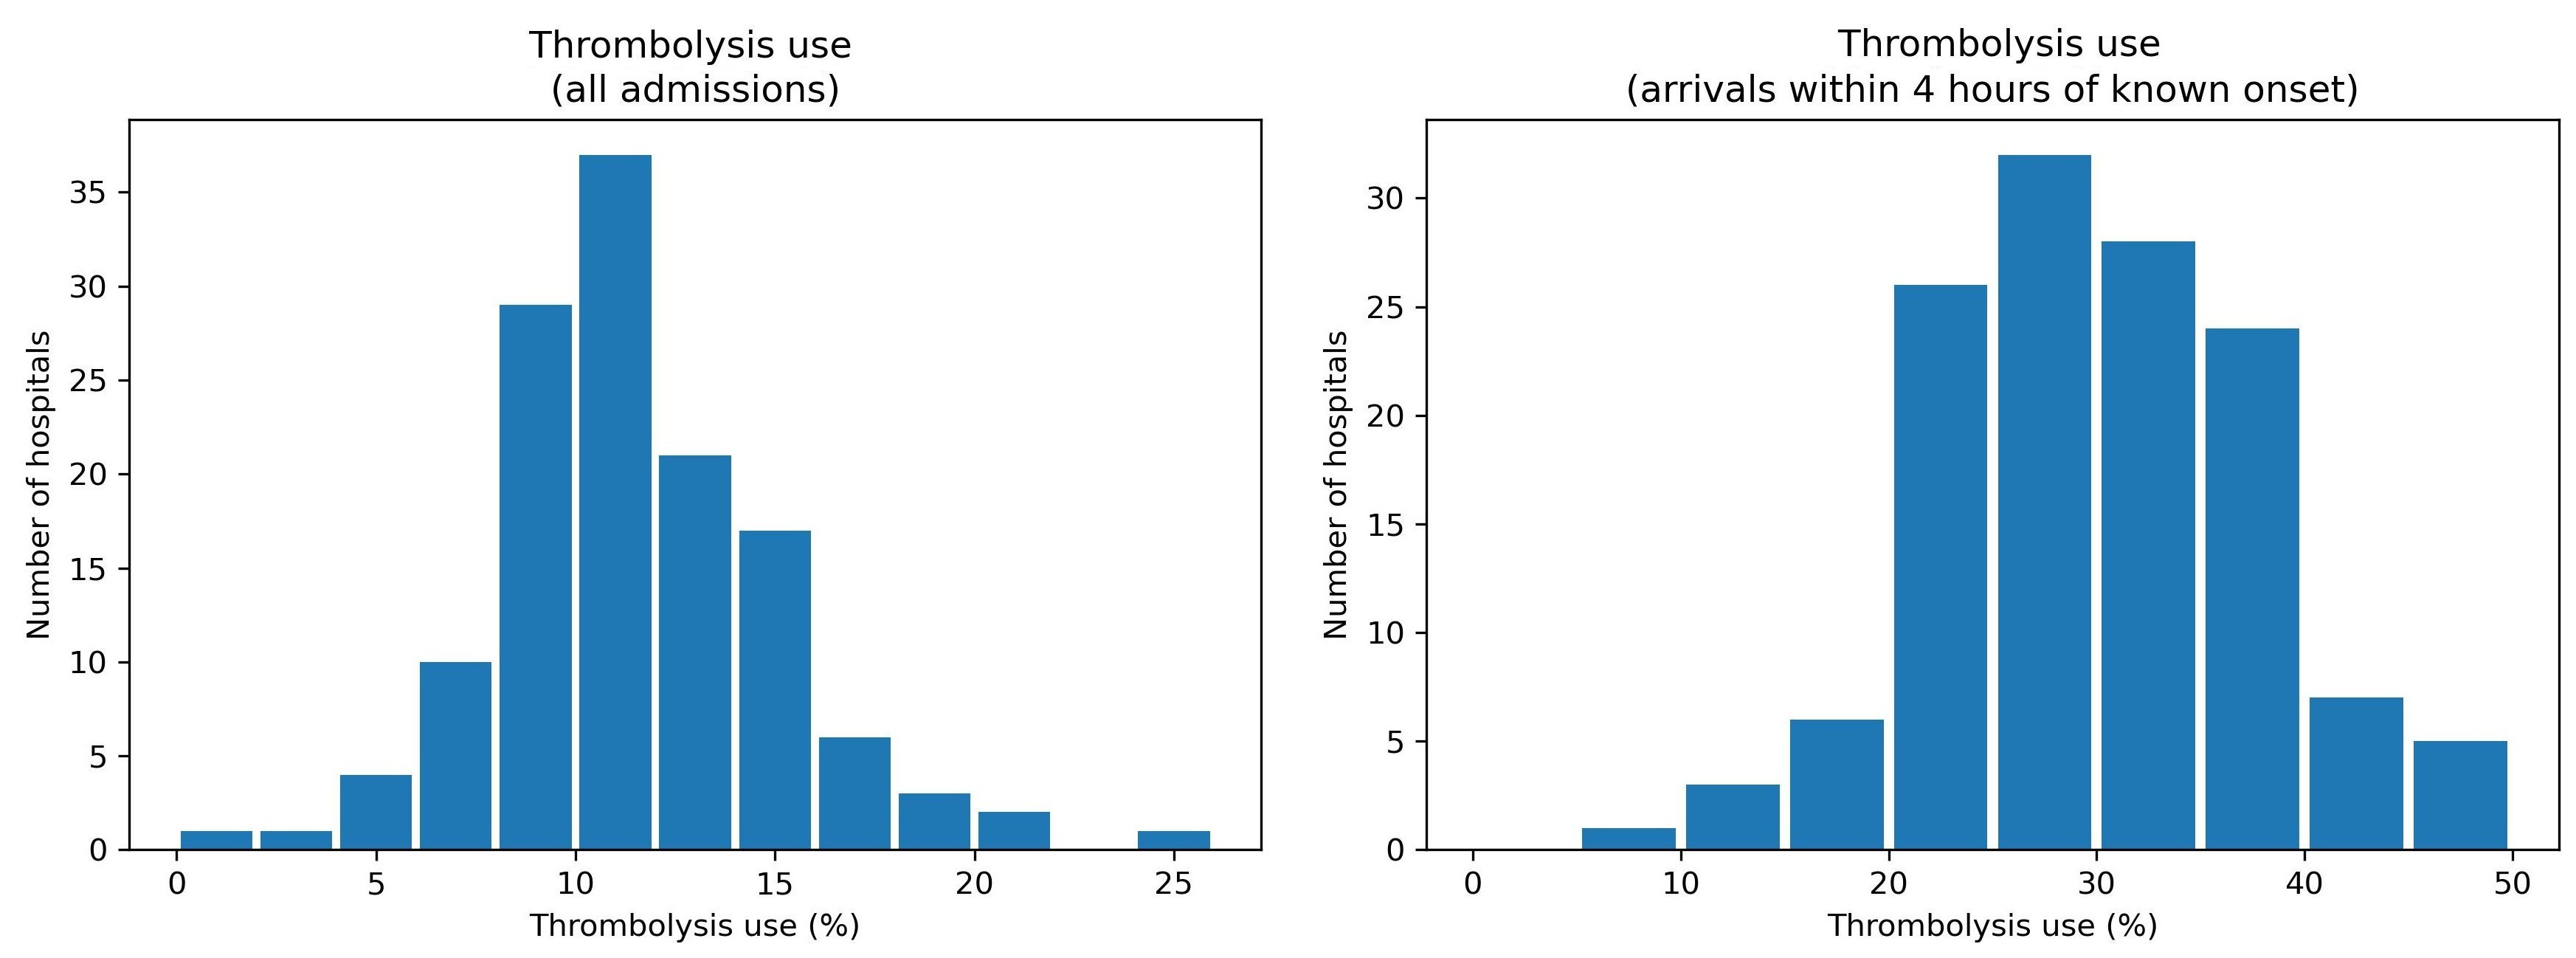
\includegraphics[width=1.0\textwidth]{./images/thrombolysis_hist}
\caption{Histogram of observed thrombolysis use in 132 hospitals. Left: Thrombolysis shown as a percentage of all emergency stroke admissions. Right: Thrombolysis shown as a percentage of those patients who arrive at hospitals within 4 hours of known stroke onset.}
\label{fig:observed_thrombolysis_appendix}
\end{figure}

%%%%%%%%%%%%%%%%%%%%%%%%%%%%%%%%%%%%%%%%%%%%%%%%%%%%%%%%%%%%%%%%%%%%%%%%%%%%%%%%%%%%%%%
\subsection{Machine learning methods}

All work was conducted in Python (v3.8). All code is available at: 

\begin{enumerate}
    \item GitHub repository: \url{https://github.com/samuel-book/samuel_shap_paper_1} \cite{samuel_paper_1_github}
    \item Jupyter book: \url{https://samuel-book.github.io/samuel_shap_paper_1/}
\end{enumerate}

Our machine learning model used XGBoost (\emph{eXtreme Gradient Boosting}, v1.5, \url{https://pypi.org/project/xgboost/}). We chose XGBoost for its efficiency, and because we working with a system with known non-linear relationships and potential feature interactions.

We used default settings apart from *learning rate* was set at 0.5 (see section \ref{sec:fine_tune}).

Machine learning models were explained using SHAP (\emph{SHapley Additive exPlanations}, v0.41 \url{https://pypi.org/project/shap/}). 

%%%%%%%%%%%%%%%%%%%%%%%%%%%%%%%%%%%%%%%%%%%%%%%%%%%%%%%%%%%%%%%%%%%%%%%%%%%%%%%%%%%%%%%

\subsection{Feature selection}

A simplified model was created by using \emph{forward feature selection} where features were added in accordance to how much each one improved the Receiver Operating Characteristic (ROC) Area Under Curve (AUC). ROC AUC was measured using stratified k-fold validation (k=5). A model with all available 84 features had an ROC AUC of 0.922. A model with 10 features had an ROC AUC of 0.919.

The 10 features selected (Figure \ref{fig:feature_selection}) were:

\begin{itemize}
    \item \emph{Arrival-to-scan time}: Time from arrival at hospital to scan (mins)
    \item \emph{Infarction}: Stroke type (1 = infarction, 0 = haemorrhage)
    \item \emph{Stroke severity}: Stroke severity (NIHSS) on arrival
    \item \emph{Precise onset time}: Onset time type (1 = precise, 0 = best estimate)
    \item \emph{Prior disability level}: Disability level (modified Rankin Scale) before stroke
    \item \emph{Stroke team}: Stroke team attended
    \item \emph{Use of AF anticoagulants}: Use of atrial fibrillation anticoagulant (1 = Yes, 0 = No)
    \item \emph{Onset-to-arrival time}: Time from onset of stroke to arrival at hospital (mins)
    \item \emph{Onset during sleep}: Did stroke occur in sleep?
    \item \emph{Age}: Age (as middle of 5 year age bands)
\end{itemize}

Stroke team was represented by a one-hot feature vector (e.g. if a patient attended hospital #2 of 5 hospitals, this is encoded as \[0, 1, 0, 0, 0\] 

\begin{figure}
\centering
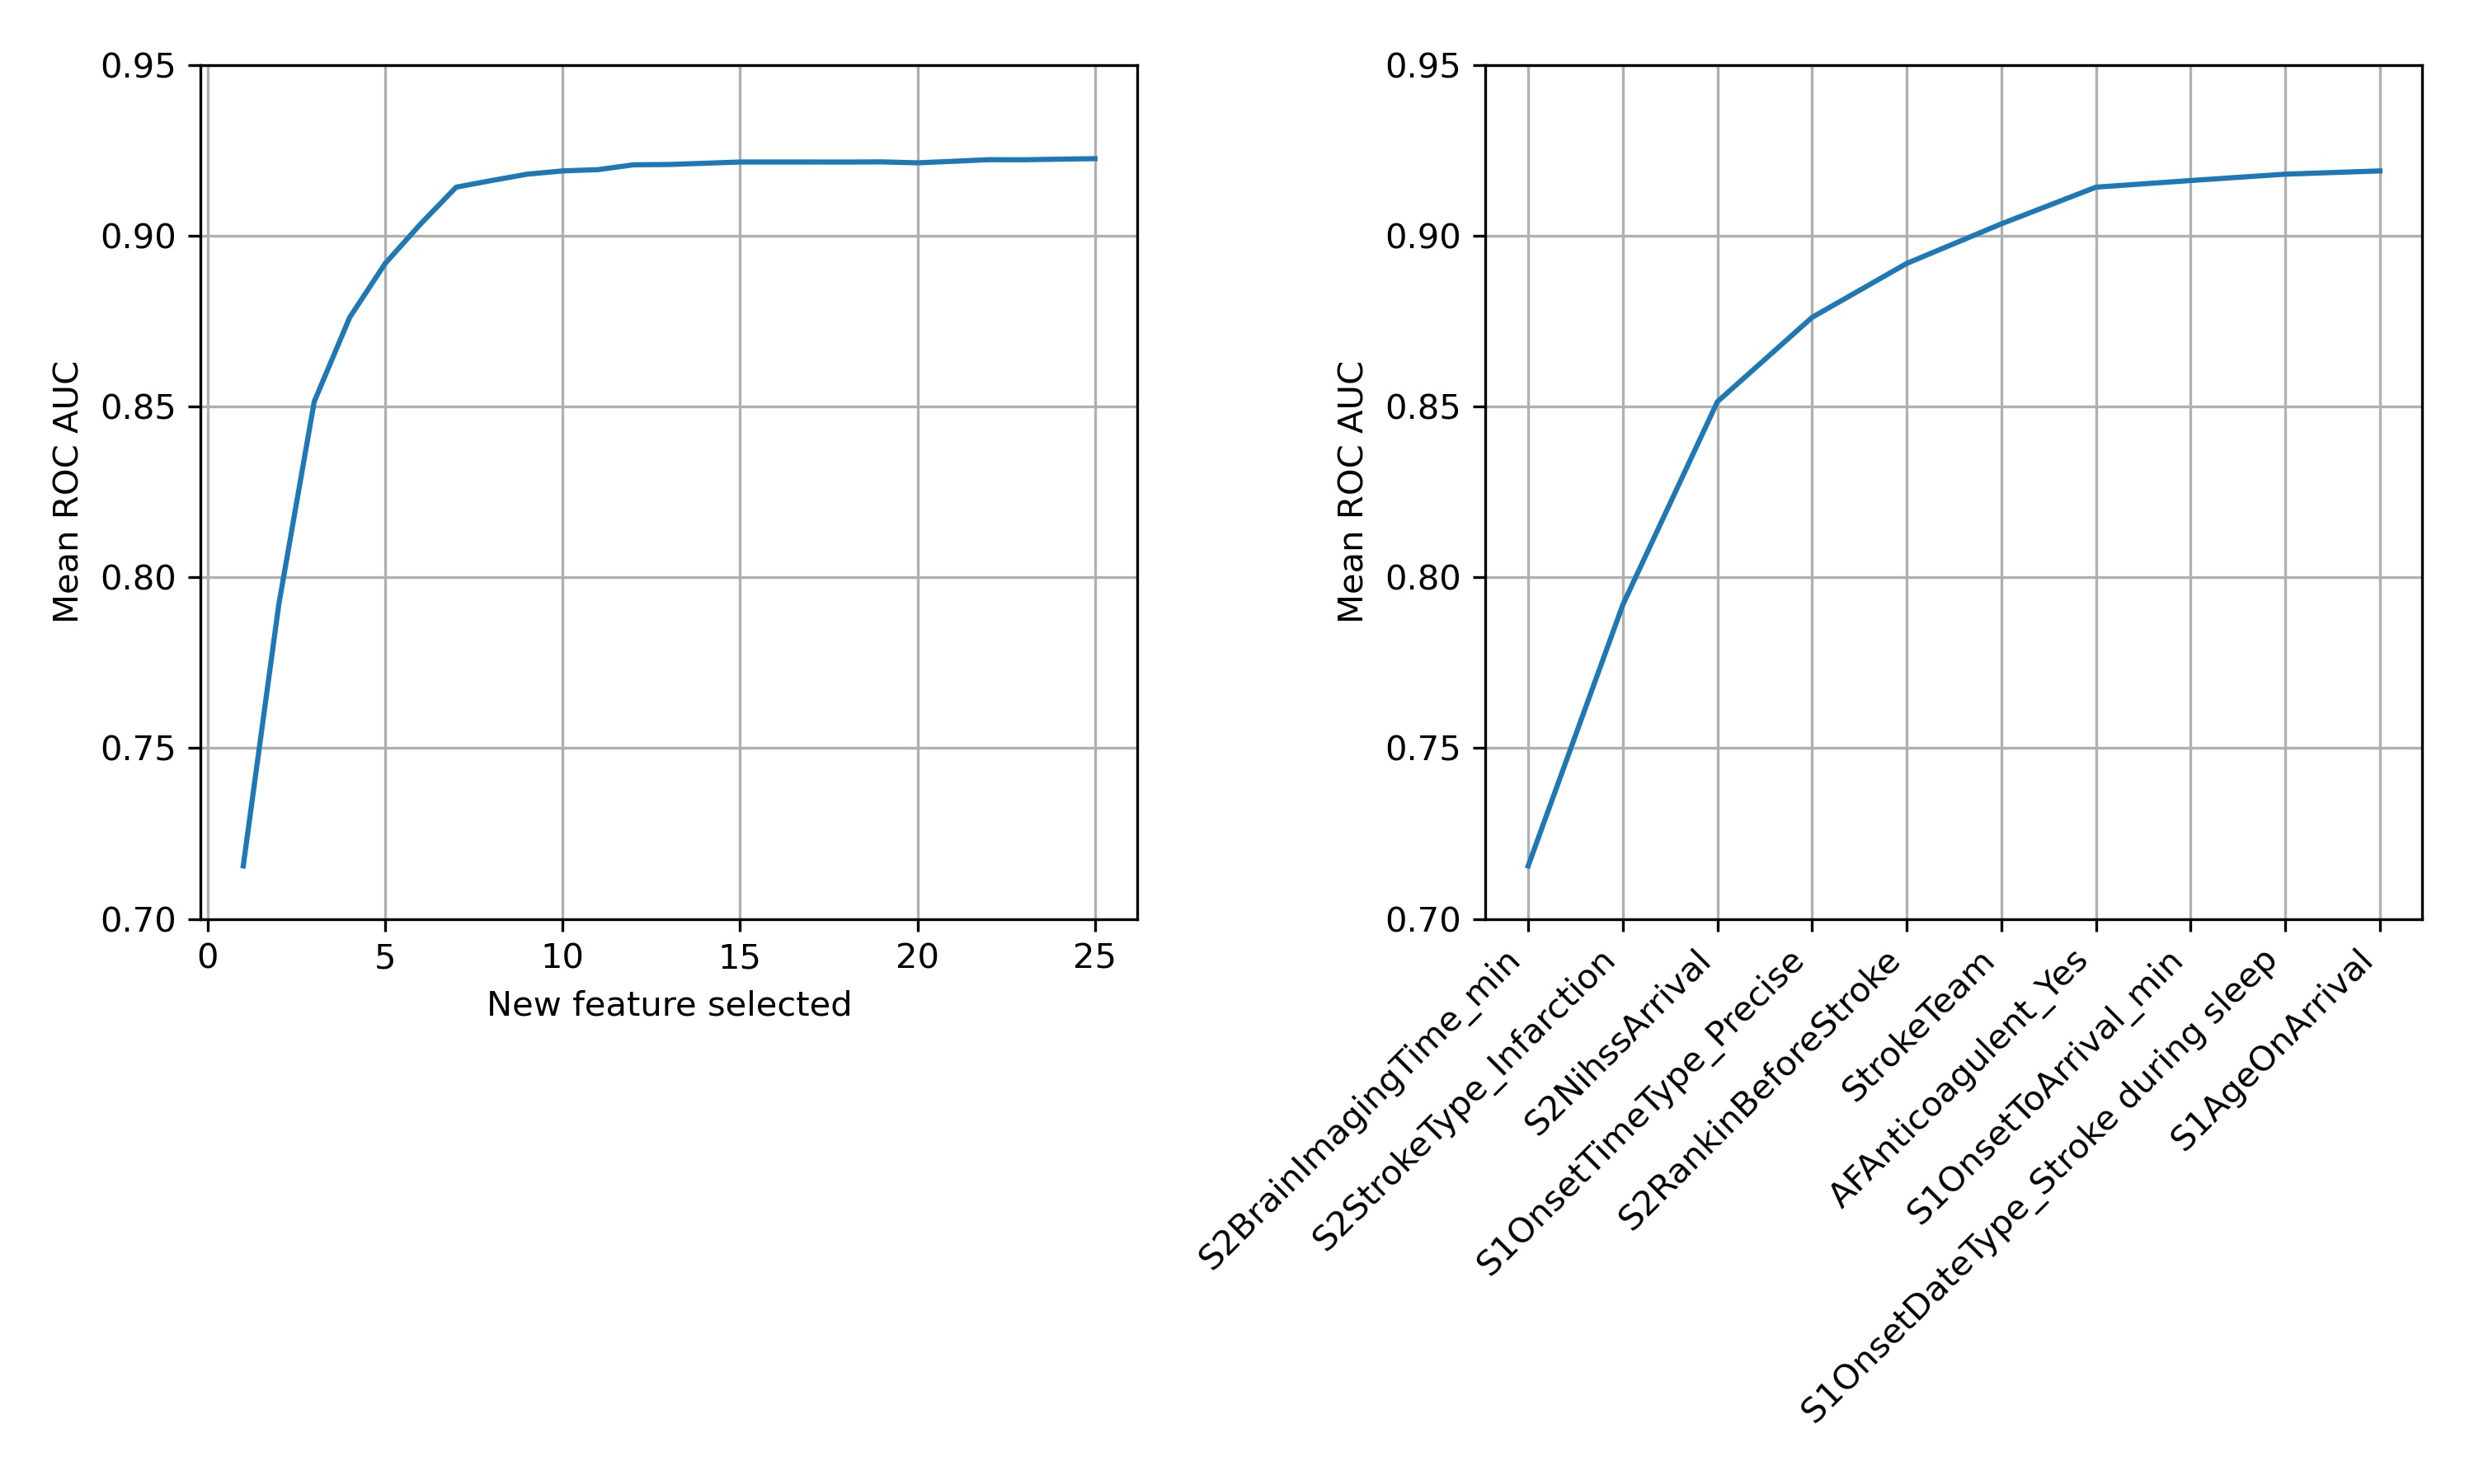
\includegraphics[width=1\textwidth]{./images/01_feature_selection}
\caption{The effect of increasing the number of features on model accuracy measured by Receiver Operating Characteristic (ROC) Area Under Curve (AUC). Left: Improvement with ROC AUC with selection of up to 25 features. Right: Improvement with ROC AUC with selection of the best 10 features. ROC was measured with stratified 5-fold cross-validation. Results show the mean of the 5-fold replicates.}
\label{fig:feature_selection}
\end{figure}


\vspace{5mm}

\begin{center}
    \textbf{\large{NOTE: All results from this point forward will use the 10 feature model.}}
\end{center}



%%%%%%%%%%%%%%%%%%%%%%%%%%%%%%%%%%%%%%%%%%%%%%%%%%%%%%%%%%%%%%%%%%%%%%%%%%%%%%%%%%%%%%%

\subsection{Correlations within the 10 selected features}

Correlations between the 10 features were measured using coefficients of determination (r-squared). All r-squared were less than 0.15, and all r-squared were less than 0.05 except 1) age and prior disability level (r-squared 0.146), and 2) onset during sleep and precise onset time (r-squared 0.078). All correlations are shown in table \ref{tab:correl}.


    
\begin{longtable}[]{@{}rrr@{}}
\caption{Correlations between the 10 features selected for the XGBoost machine learning model.}\\
\toprule
Variable 1 & Variable 2 & r-squared\tabularnewline
\midrule
\endhead
Age & Prior disability level & 0.1462\tabularnewline
Onset during sleep & Precise onset time & 0.0784\tabularnewline
Stroke severity & Prior disability level & 0.0454\tabularnewline
Stroke severity & Infarction & 0.0386\tabularnewline
Precise onset time & Onset-to-arrival time & 0.0344\tabularnewline
Stroke severity & Age & 0.0268\tabularnewline
Age & Use of AF anticoagulants & 0.0207\tabularnewline
Stroke severity & Onset-to-arrival time & 0.0186\tabularnewline
Precise onset time & Prior disability level & 0.0131\tabularnewline
Age & Precise onset time & 0.0090\tabularnewline
Prior disability level & Use of AF anticoagulants &
0.0070\tabularnewline
Onset during sleep & Onset-to-arrival time & 0.0043\tabularnewline
Onset-to-arrival time & Age & 0.0038\tabularnewline
Use of AF anticoagulants & Infarction & 0.0033\tabularnewline
Prior disability level & Onset-to-arrival time & 0.0022\tabularnewline
Precise onset time & Arrival-to-scan time & 0.0021\tabularnewline
Use of AF anticoagulants & Stroke severity & 0.0019\tabularnewline
Arrival-to-scan time & Stroke severity & 0.0019\tabularnewline
Precise onset time & Use of AF anticoagulants & 0.0016\tabularnewline
Stroke severity & Onset during sleep & 0.0011\tabularnewline
Infarction & Onset-to-arrival time & 0.0007\tabularnewline
Infarction & Onset during sleep & 0.0007\tabularnewline
Infarction & Precise onset time & 0.0006\tabularnewline
Onset-to-arrival time & Arrival-to-scan time & 0.0004\tabularnewline
Arrival-to-scan time & Prior disability level & 0.0001\tabularnewline
Onset-to-arrival time & Use of AF anticoagulants & 0.0001\tabularnewline
Stroke severity & Precise onset time & 0.0000\tabularnewline
Arrival-to-scan time & Age & 0.0000\tabularnewline
Use of AF anticoagulants & Onset during sleep & 0.0000\tabularnewline
Prior disability level & Onset during sleep & 0.0000\tabularnewline
Infarction & Age & 0.0000\tabularnewline
Use of AF anticoagulants & Arrival-to-scan time & 0.0000\tabularnewline
Onset during sleep & Arrival-to-scan time & 0.0000\tabularnewline
Arrival-to-scan time & Infarction & 0.0000\tabularnewline
Age & Onset during sleep & 0.0000\tabularnewline
Prior disability level & Infarction & 0.0000\tabularnewline
\bottomrule
\label{tab:correl}
\end{longtable}



%%%%%%%%%%%%%%%%%%%%%%%%%%%%%%%%%%%%%%%%%%%%%%%%%%%%%%%%%%%%%%%%%%%%%%%%%%%%%%%%%%%%%%%

\subsection{Model accuracy}

Model accuracy was measured using stratified 5-fold cross validation. The key results are shown in table \ref{tab:accuracy_appendix}.

\begin{minipage}{\textwidth}
\begin{longtable}[]{@{}lll@{}}
\caption{Accuracy of 10 feature XGBoost model in predicting thrombolysis use in patients arriving at hospital within 4 hours of known stroke onset.}\\
\toprule
Accuracy measurement & mean & std\tabularnewline
\midrule
\endhead
Actual positive rate & 0.296 & 0.000\tabularnewline
Actual negative rate & 0.704 & 0.000\tabularnewline
Predicted positive rate & 0.294 & 0.002\tabularnewline
Predicted negative rate & 0.706 & 0.002\tabularnewline
Accuracy & 0.850 & 0.004\tabularnewline
Sensitivity (recall) & 0.743 & 0.004\tabularnewline
Specificity & 0.894 & 0.004\tabularnewline
Precision & 0.747 & 0.007\tabularnewline
ROC AUC & 0.918 & 0.003\tabularnewline
Balanced sensitivity/specificity & 0.839 & 0.003\tabularnewline
\bottomrule
\label{tab:accuracy_appendix}
\end{longtable}
\end{minipage}

We found an overall accuracy of 85.0\%, with a balanced accuracy. The predicted thrombolysis rate of 29.4\% was very close to the observed thrombolysis rate of 29.6\%.

Figure \ref{fig:roc} shows the receiver operating characteristic curve, along with the trade-off between sensitivity and specificity.

\begin{figure}
\centering
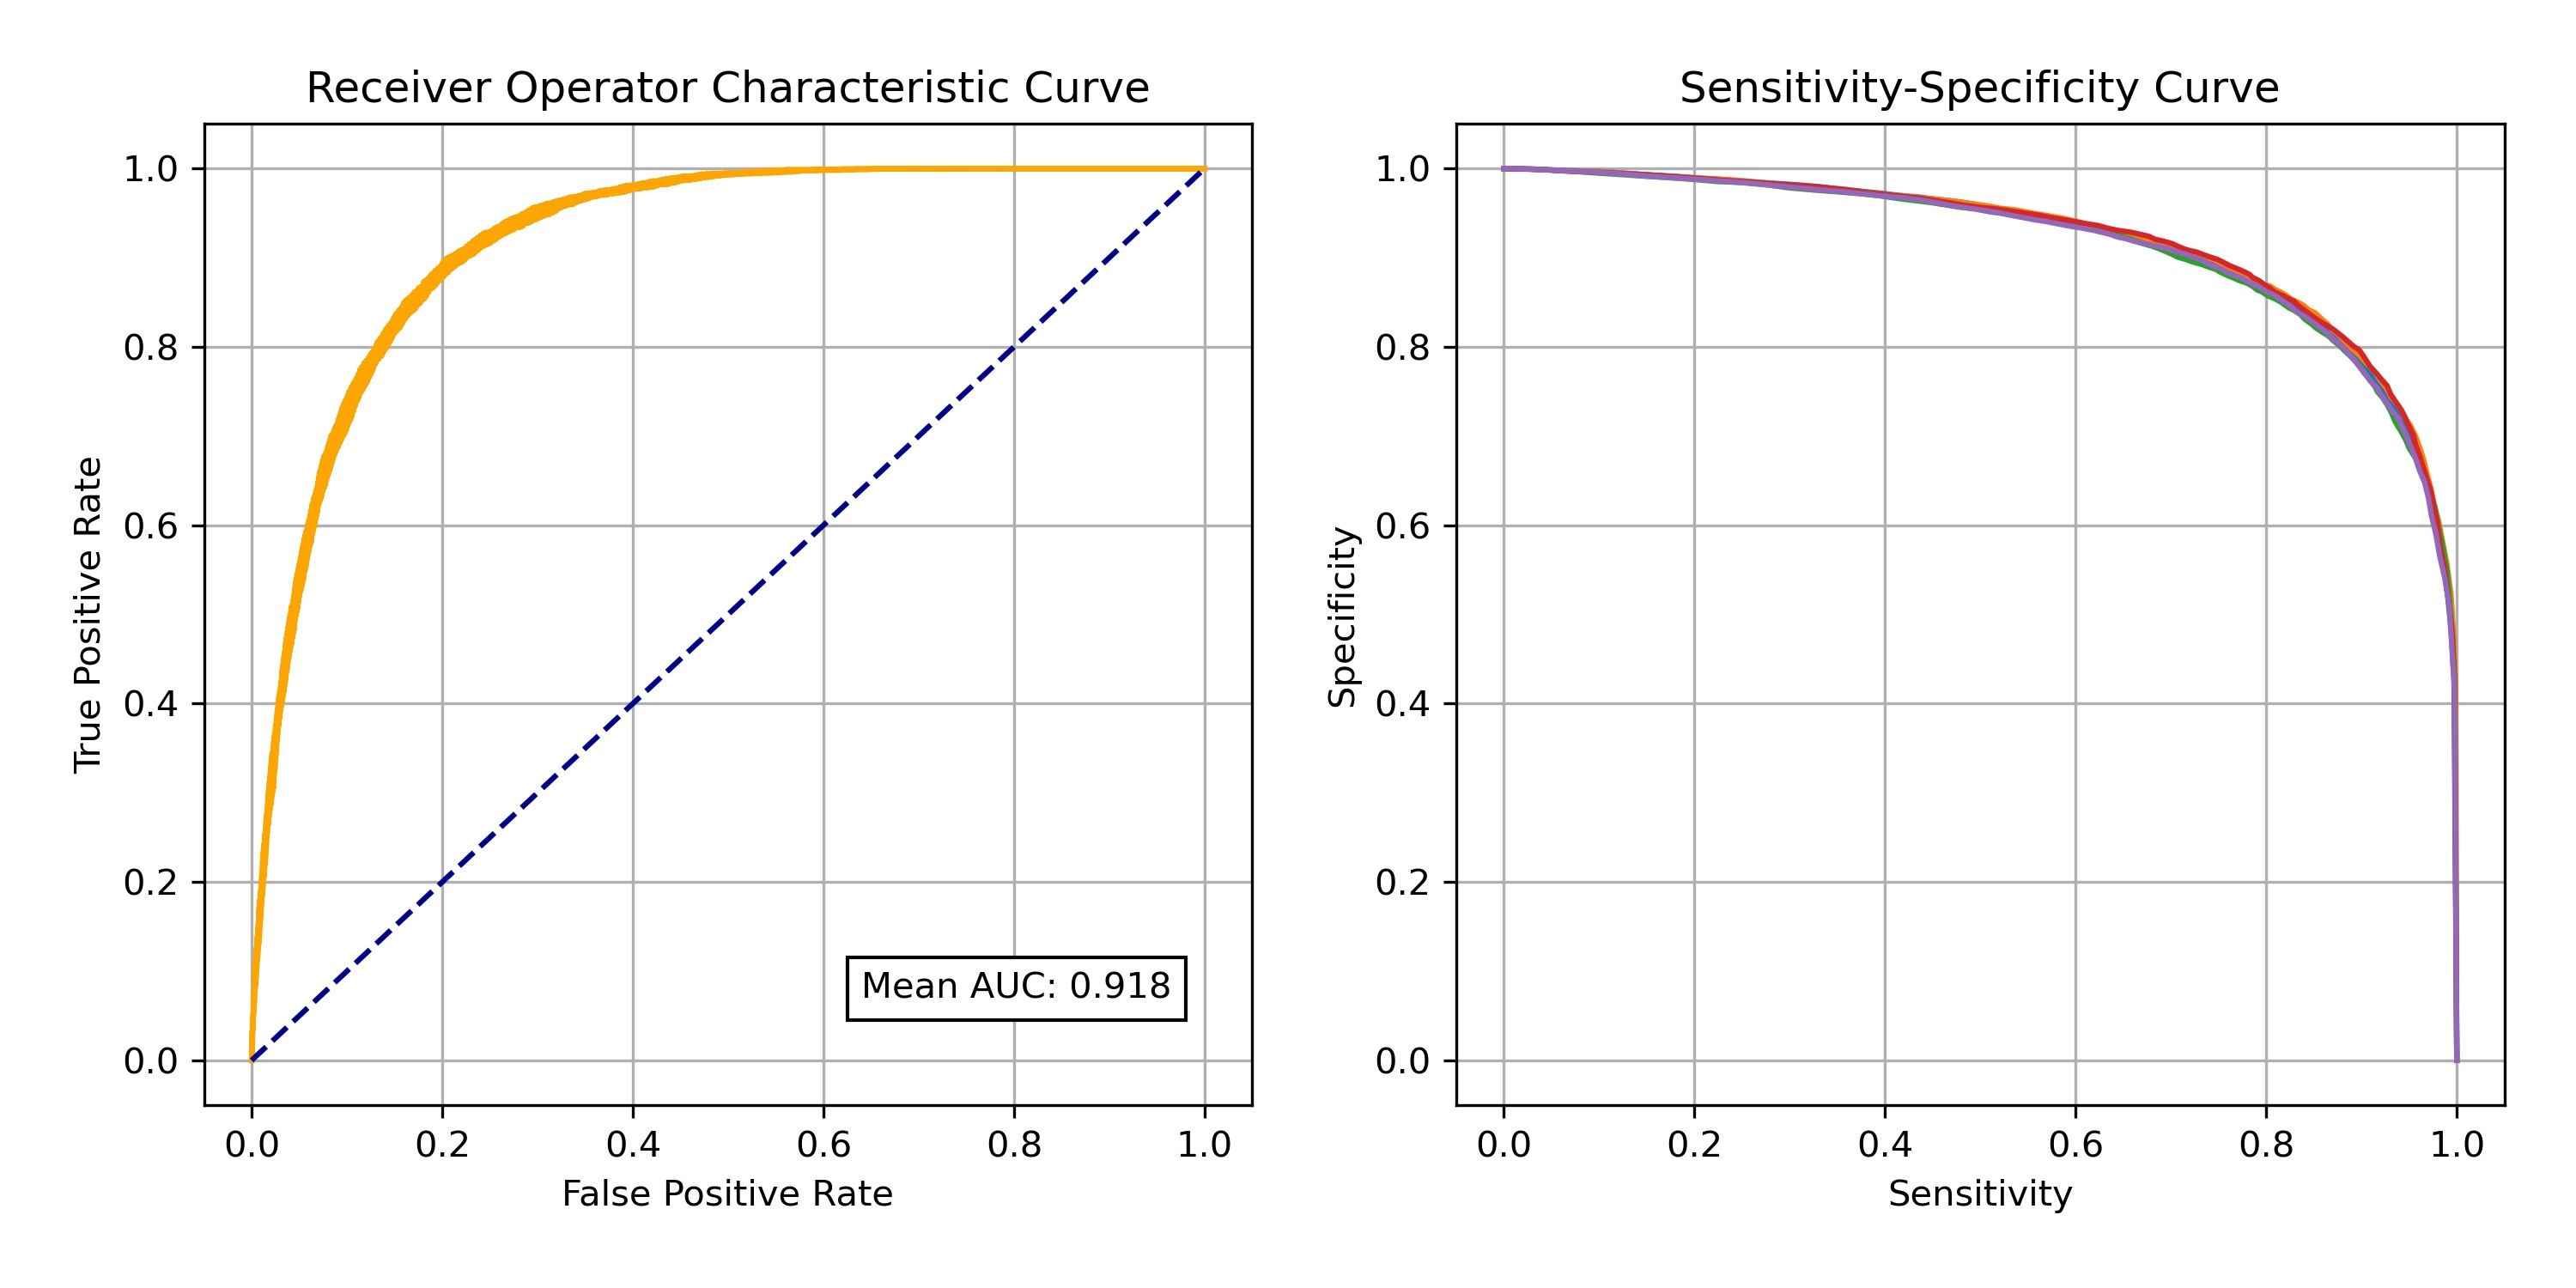
\includegraphics[width=1\textwidth]{./images/02_xgb_10_features_roc_sens_spec}
\caption{Model accuracy of a XGBoost model using 10 features. Left: Receiver Operating Characteristic (ROC) Area Under Curve (AUC). Right: The trade-off between Sensitivity and Specificity. Accuracy was measured with stratified 5-fold cross-validation, and both charts show all 5 k-fold replicates.}
\label{fig:roc}
\end{figure}


%%%%%%%%%%%%%%%%%%%%%%%%%%%%%%%%%%%%%%%%%%%%%%%%%%%%%%%%%%%%%%%%%%%%%%%%%%%%%%%%%%%%%%%

\subsection{Model calibration}

The model calibration was checked by binning predictions by probability, and comparing the mean predicted probability with the fraction that were actually positive (table \ref{tab:calibration} and figure \ref{fig:calibration}). In a well-calibrated model, in each bin the average probability of receiving thrombolysis should be close to the proportion of patients who actually received thrombolysis. Results demonstrated that the model was naturally well-calibrated, and was not in need of any calibration correction. As expected, the fraction of predictions that were correct is related to the predicted probability of receiving thrombolysis (when predictions were close to 50\% probability of receiving thrombolysis the model was correct about 50\% of the time, whereas when the model had predictions of less than 10\% or greater than 90\% probability of receiving thrombolysis, the model was be correct about 90\% of the time).

Nearly 50\% of patients fell in the 0-10\% probability of receiving thrombolysis - that is the model gave a confident prediction that the these patients would not receive thrombolysis, with the model being correct in these predictions 98\% of the time.

\begin{minipage}{\textwidth}
\begin{longtable}[]{@{}lllll@{}}
\caption{Model calibration based on binning by predicted probability of thrombolysis.}\\
\toprule
Bin & Predicted probability & Fraction positive & Fraction correct &
Frequency\tabularnewline
\midrule
\endhead
0.0 - 0.1 & 0.018 & 0.023 & 0.977 & 0.480\tabularnewline
0.1 - 0.2 & 0.146 & 0.174 & 0.826 & 0.082\tabularnewline
0.2 - 0.3 & 0.248 & 0.271 & 0.729 & 0.056\tabularnewline
0.3 - 0.4 & 0.348 & 0.371 & 0.629 & 0.045\tabularnewline
0.4 - 0.5 & 0.450 & 0.443 & 0.557 & 0.043\tabularnewline
0.5 - 0.6 & 0.551 & 0.546 & 0.546 & 0.042\tabularnewline
0.6 - 0.7 & 0.652 & 0.643 & 0.643 & 0.049\tabularnewline
0.7 - 0.8 & 0.753 & 0.736 & 0.736 & 0.065\tabularnewline
0.8 - 0.9 & 0.852 & 0.827 & 0.827 & 0.089\tabularnewline
0.9 - 1.0 & 0.932 & 0.893 & 0.893 & 0.049\tabularnewline
\bottomrule
\label{tab:calibration}
\end{longtable}
\end{minipage}


\begin{figure}
\centering
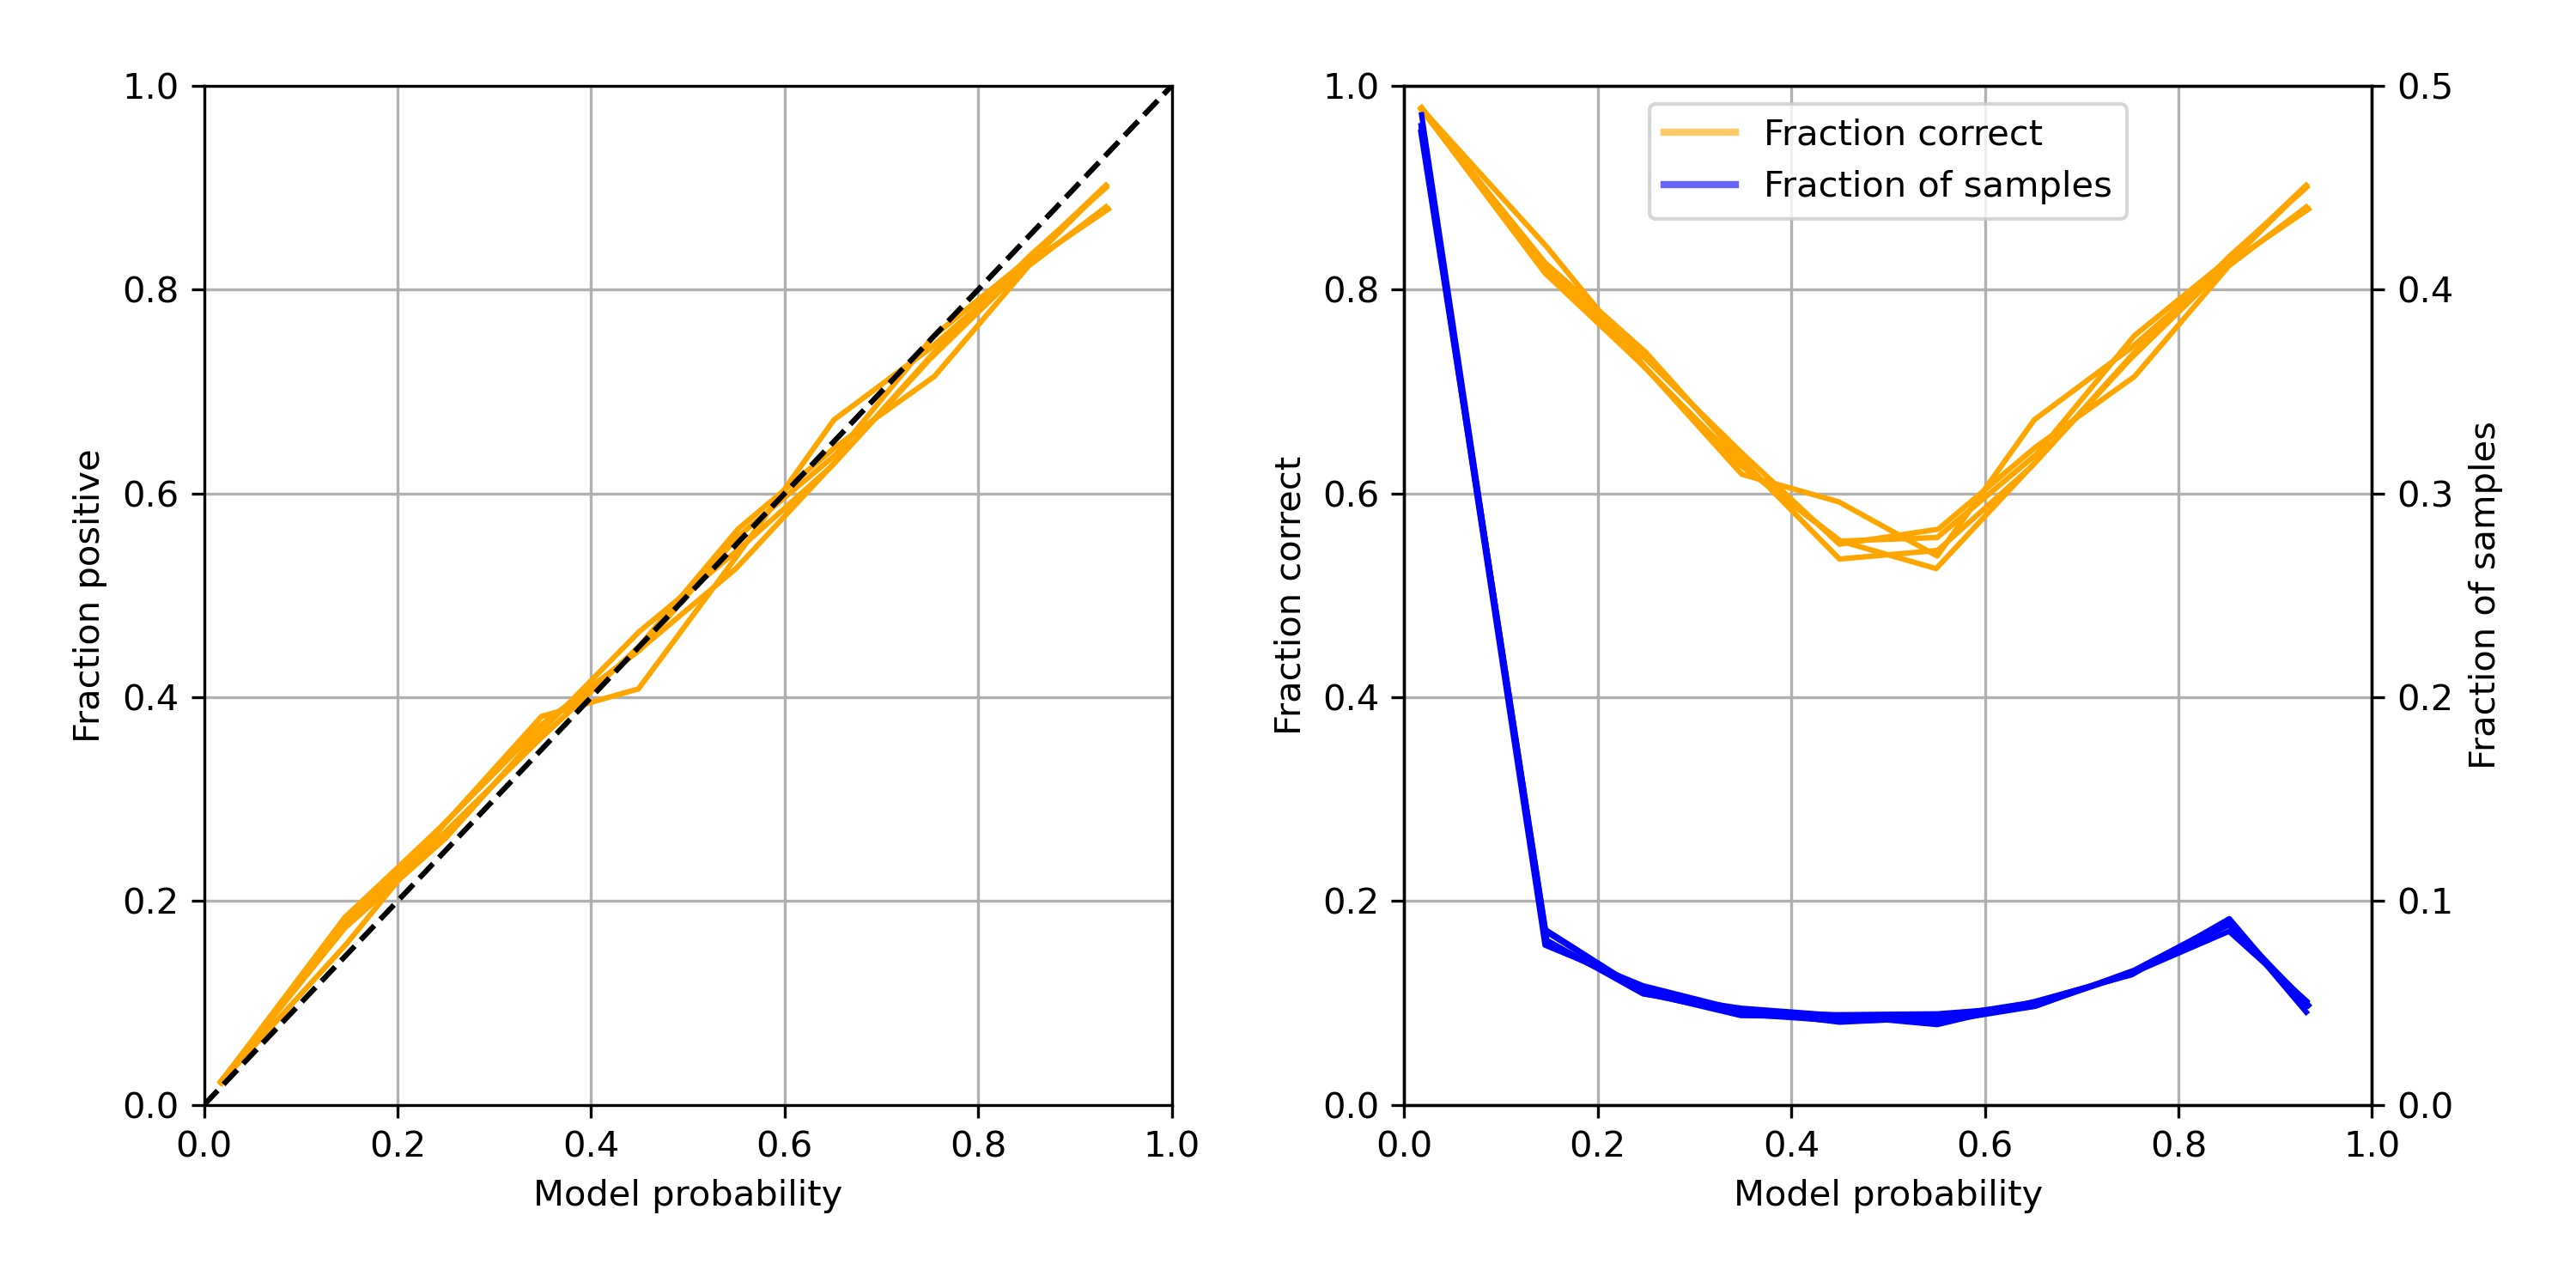
\includegraphics[width=1\textwidth]{./images/02_xgb_10_features_reliability}
\caption{Calibration check of the model. Left: The proportion of patients receiving thrombolysis for binned probability of receiving thrombolysis. Right: The proportion of predictions in each bin (blue), and the proportion of predictions that are correct (orange). Plot show results for all 5 k-fold replicates.}
\label{fig:calibration}
\end{figure}


%%%%%%%%%%%%%%%%%%%%%%%%%%%%%%%%%%%%%%%%%%%%%%%%%%%%%%%%%%%%%%%%%%%%%%%%%%%%%%%%%%%%%%%

\subsection{Evaluating variation in model predictions and predicted 10k cohort thrombolysis rate using bootstrap models}

Data was split into a training set of 78,928 patients, and a test set of 10k patients. 30 models were trained, each with a different bootstrap sample of the training set and with a different model random seed. For each of the 10k test set, we evaluated the variation in the predicted probability of receiving thrombolysis (figure \ref{fig:bootstrap_1}). The mean of these standard deviations was 0.057, but the variation depended on the probability, with variation peaking at about 0.13 when the prediction probability of receiving thrombolysis was around 0.5.

\begin{figure}
\centering
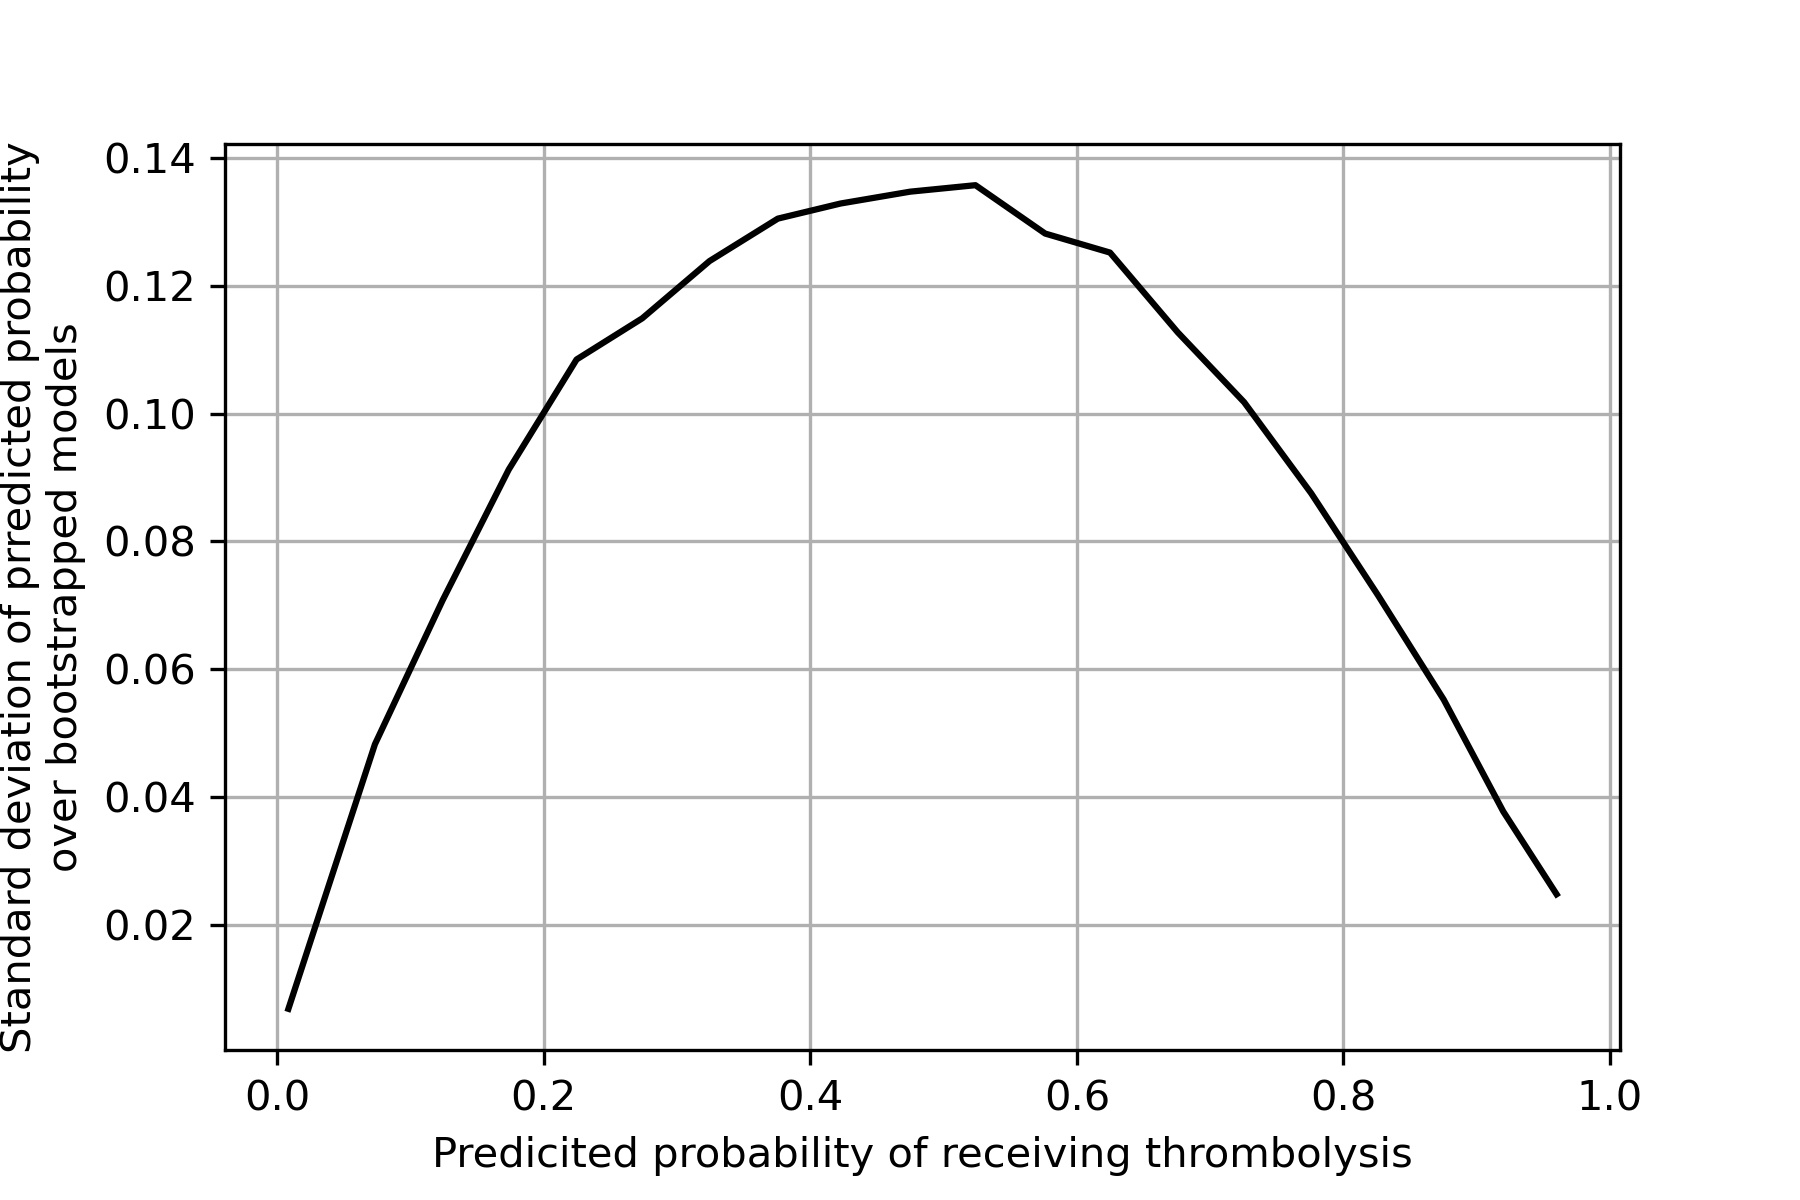
\includegraphics[width=0.7\textwidth]{./images/50_xgb_10_features_10k_cohort_bootstrap_prediction_sd}
\caption{Standard deviation of predicted probability of receiving thrombolysis, from 30 bootstrapped models predicting the probability of receiving thrombolysis in 10k patients. Results are binned by predicted probability.}
\label{fig:bootstrap_1}
\end{figure}

Additionally, we used the models and test set to predict thrombolysis use at each of the 132 hospitals if the 10k cohort of patients had attended each of the hospitals (by changing the hospital one-hot encoding, figure \ref{fig:bootstrap_2}). We predicted the thrombolysis use at each hospital, and examined the variation between the 30 bootstrapped models. The mean of the standard deviation of bootstrap replicates was 1.7\% (where hospital thrombolysis use rates were 10\% to 45\%).

\begin{figure}
\centering
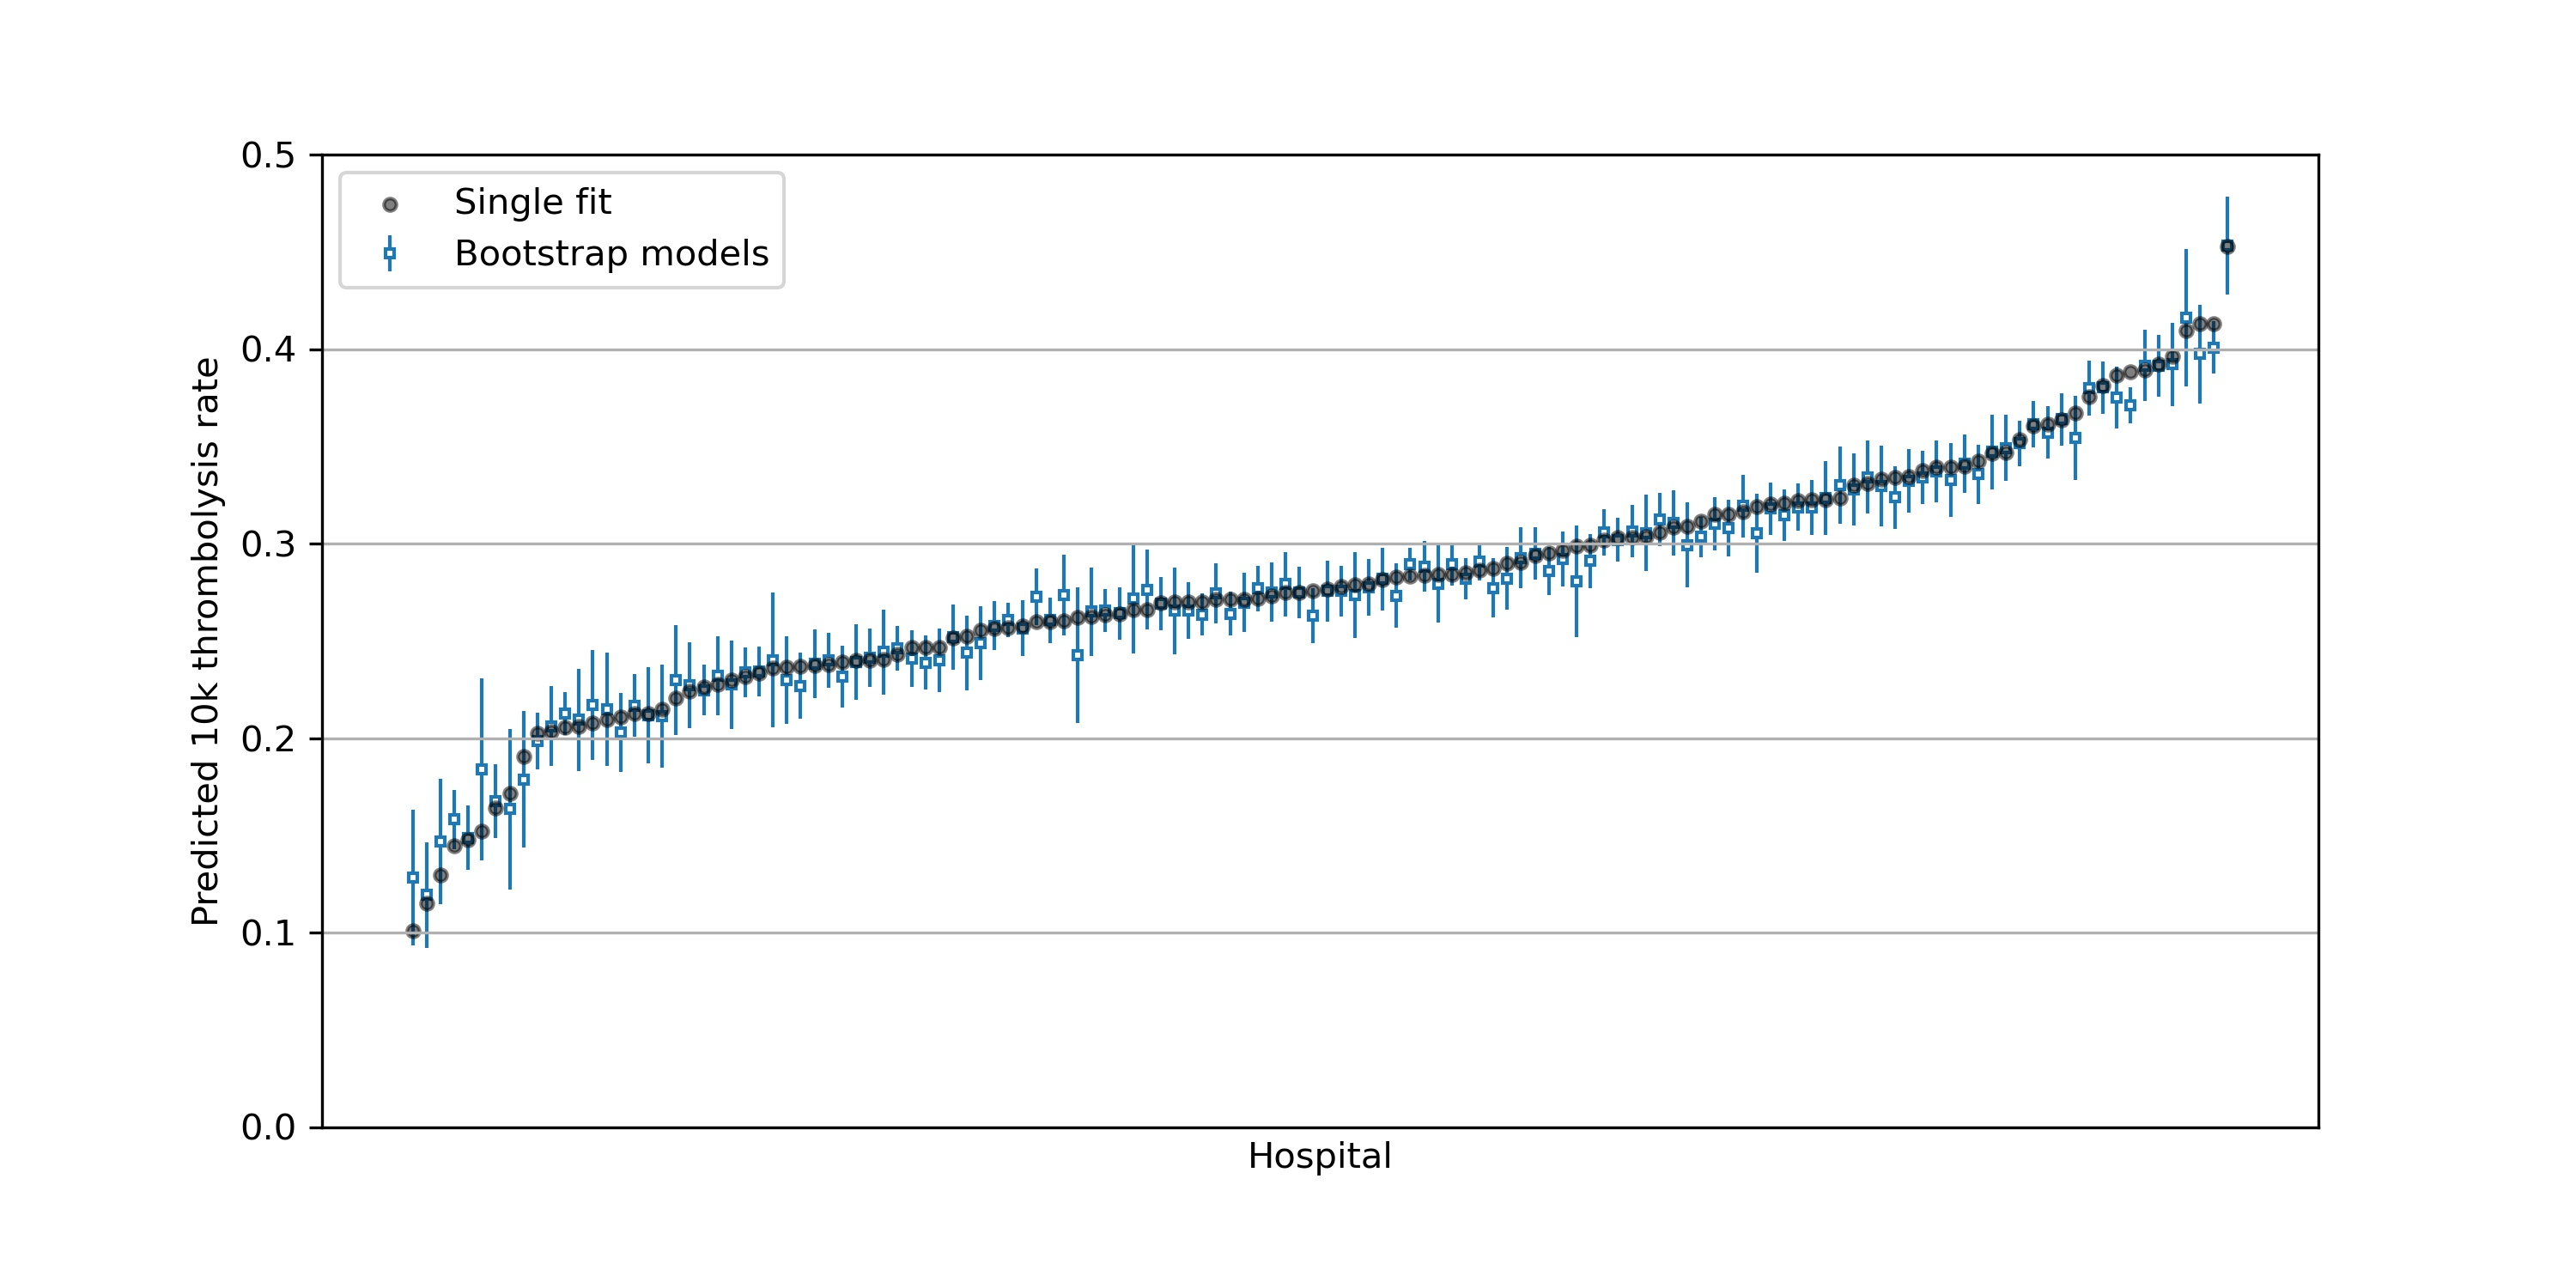
\includegraphics[width=1\textwidth]{./images/50_xgb_10_features_10k_cohort_bootstrap_10k_sd}
\caption{Mean and standard deviation of predicted thrombolysis use at 132 hospitals from 30 bootstrapped models. Results are for predicted thrombolysis use for the same 10k patient cohort for each hospital. In addition to the results for the bagging models, the predicted thrombolysis use for a single model with bootstrap sampling is shown. Results are ordered by thrombolysis use at each hospital predicted from the single non-bootstrap model.}
\label{fig:bootstrap_2}
\end{figure}

Bagging experiments were repeated with \emph{Baysian Bootstrapping} based on weighting training samples using a Dirichlet distribution. Very similar results were achieved, with a mean standard deviation of bootstrap replicate probability predictions of 0.054, and a mean standard deviation of bootstrap replicate 10k thrombolysis use in hospitals of 1.6\%.

The evaluation of bootstrapped replicates gave us confidence that a single model fit would be sufficient. 


%%%%%%%%%%%%%%%%%%%%%%%%%%%%%%%%%%%%%%%%%%%%%%%%%%%%%%%%%%%%%%%%%%%%%%%%%%%%%%%%%%%%%%%

\subsection{Learning curves}

Learning curves evaluate the relationship between training set size and model accuracy. Learning curves were performed using stratified 5-fold validation, and by random sampling (without replacement) of the training set (figure \ref{fig:learning_curve}. The maximum accuracy achieved was 85\% using 70k training instances, 82.5\% accuracy was achieved with 4k training instances. There was a shallow improvement between 4k and 70k training points.

\begin{figure}
\centering
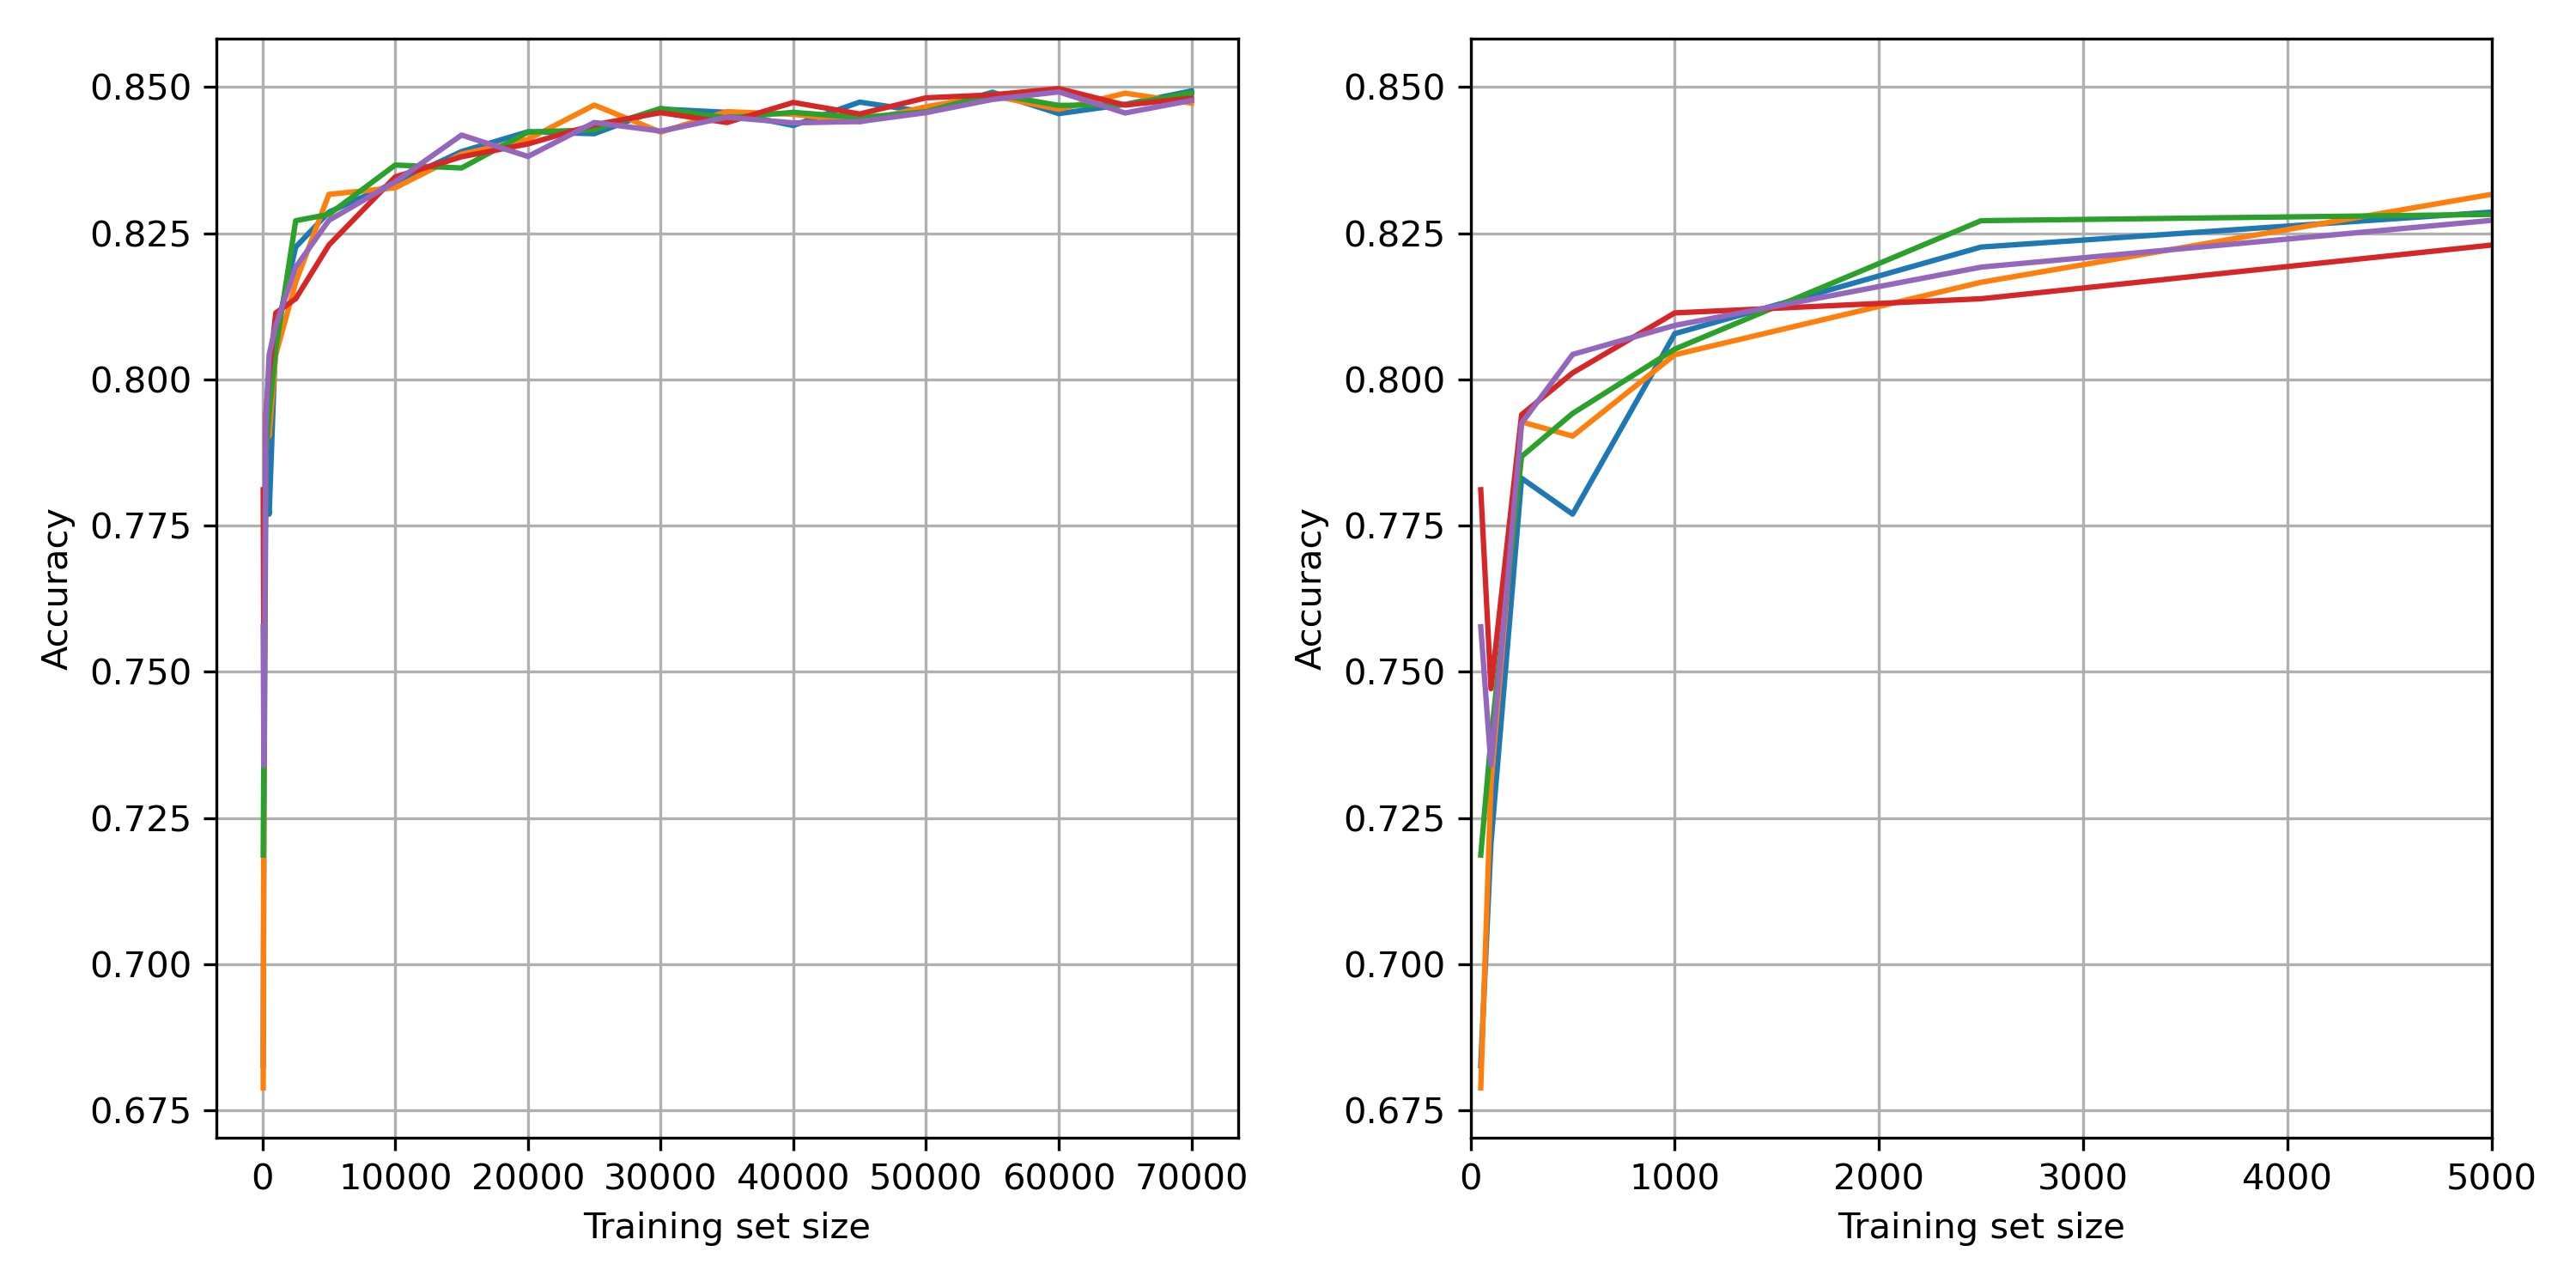
\includegraphics[width=1\textwidth]{./images/02_xgb_10_features_learning_curve}
\caption{Learning curves showing the relationship between training set size and model accuracy. Left: training set size up to 70k. Right: training set size up to 5k (same results as the results on the left). Results are shown for all 5 k-fold replicates.}
\label{fig:learning_curve}
\end{figure}

%%%%%%%%%%%%%%%%%%%%%%%%%%%%%%%%%%%%%%%%%%%%%%%%%%%%%%%%%%%%%%%%%%%%%%%%%%%%%%%%%%%%%%%

\subsection{Fine-tuning of model regularisation}
\label{sec:fine_tune}

As hospital ID is encoded as one-hot, and there are 132 hospitals, it is possible that the effect of hospitals ID becomes 'regularised out', especially as for each one-hot encoded column about 99% of the feature values will be zero. *Learning rate* in XGBoost acts as a regularising method. The lower the learning rate the less weight new trees have, and so the model becomes more regularised (less likely to overfit).

As we are concerned with differences between hospitals, we did not want to over-regularise the model. To optimise *learning rate* we looked at the between-hospital variation of predicted thrombolysis use in a 10k cohort of patients (with the model predicting the use of thrombolysis in each hospital with the same 10k cohort). The model was trained on the remaining 78,928 patients, with varying learning rates (figure \ref{fig:learning_rate} and table \ref{tab:learning_rate}).

Reducing the learning rate below 0.5 led to reduced between-hospital variation in the predicted use of thrombolysis, suggesting that the effect of hospital ID was being reduced by over-regularisation. 

A learning rate of 0.5 was chosen for all modelling (including the accuracy measurements above).

\begin{figure}
\centering
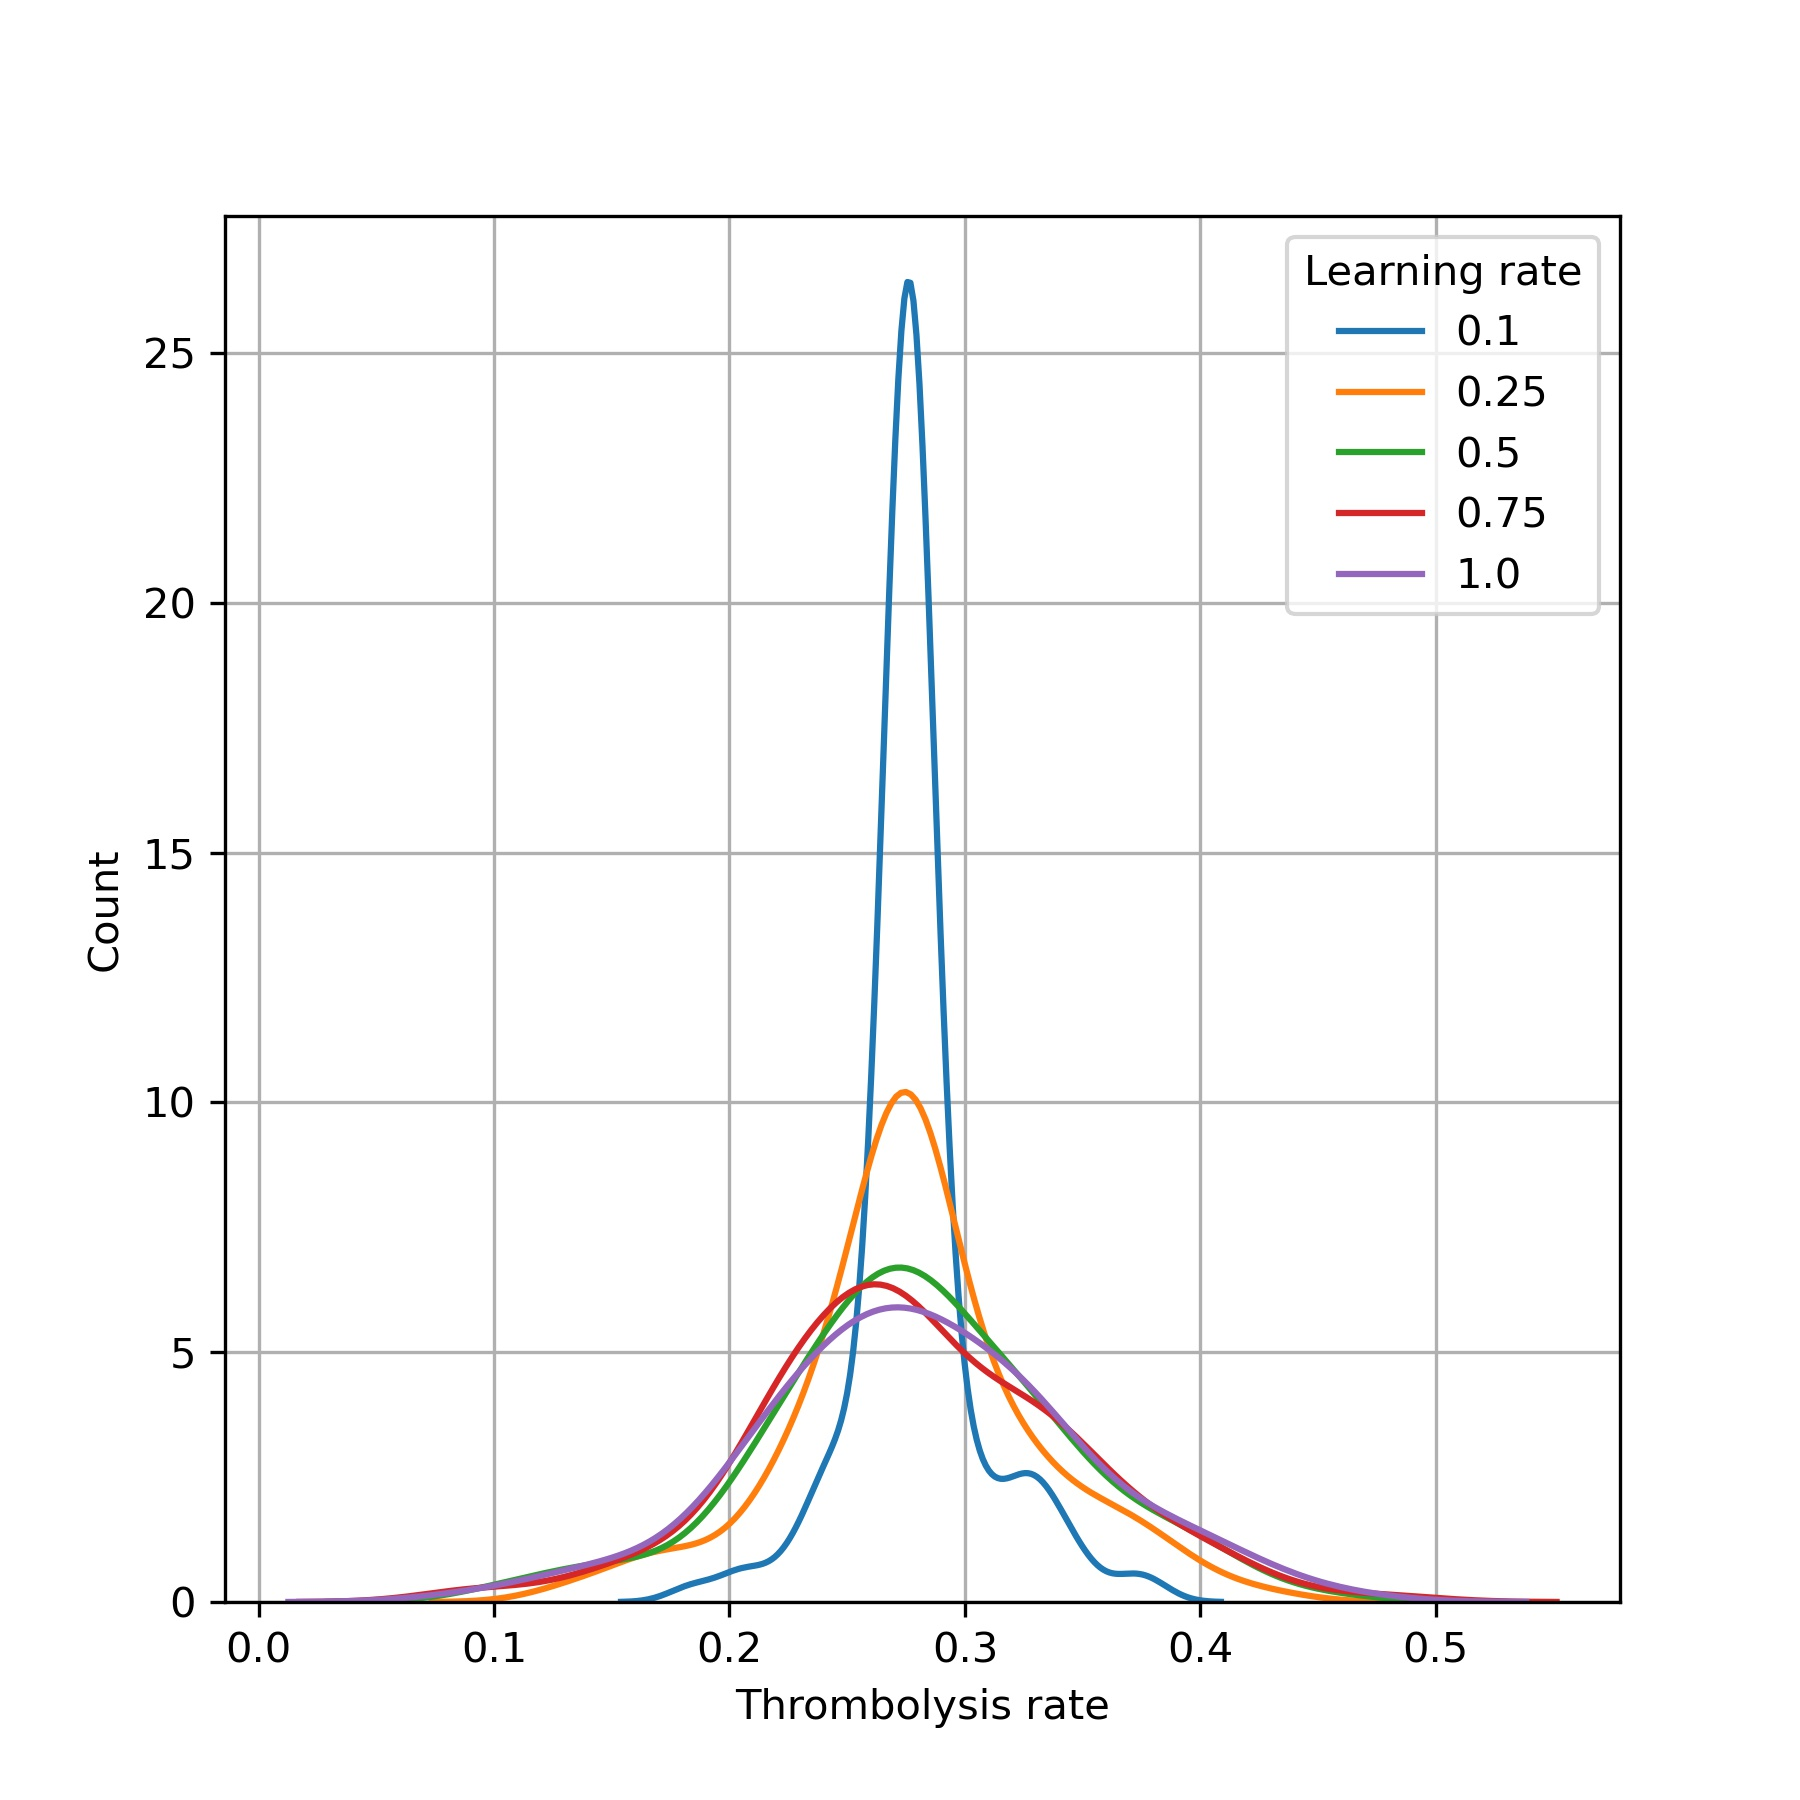
\includegraphics[width=0.7\textwidth]{./images/91_learning_rate}
\caption{Effect of adjusting XGBoost learning rate on the distribution predicted thrombolysis use across 132 hospitals. A narrower distribution indicates that hospital thrombolysis rates are tending towards the mean thrombolysis hospital rate.}
\label{fig:learning_rate}
\end{figure}

\begin{minipage}{\textwidth}
\begin{longtable}[]{@{}llllll@{}}
\caption{Statistics on the variation in predicted thrombolysis use between hospitals, with varying learning rate}\\
\toprule
Learning rate & 0.1 & 0.25 & 0.5 & 0.75 & 1.0\tabularnewline
\midrule
\endhead
Mean & 0.28 & 0.28 & 0.28 & 0.28 & 0.28\tabularnewline
StdDev & 0.03 & 0.05 & 0.06 & 0.07 & 0.07\tabularnewline
Min & 0.18 & 0.13 & 0.10 & 0.09 & 0.09\tabularnewline
Max & 0.38 & 0.43 & 0.45 & 0.48 & 0.46\tabularnewline
\bottomrule
\label{tab:learning_rate}
\end{longtable}
\end{minipage}

\subsection*{Acknowledgements}

We would like to thank the SAMueL project team (Lauren Asare, Julia Frost, Iain Lang, Kristin Liabo, Peter McMeekin, Keira Pratt-Boyden, Cathy Pope, Ken Stein, Penny Thompson) for their input into this work.

We would also like to thank our Patient and Carer Involvement team led by Leon Farmer (David Burgess, Simon Douglas, Ian Hancock, Nicola Hancock, John Williams), and our expert advisory group (Ajay Bhalla, Gary Ford, Anthony Rudd, and Martin Utley).
%%%%%%%%%%%%%%%%%%%%%%%%%%%%%%%%%%%%%%%%%%%%%%%%%%%%%%%%%%%%%%%%%%%%%%%%%%%%%%%%%%%%%%%
%TC:endignore

\end{document}